\setcounter{figure}{0}
\setcounter{table}{0}

\begin{figure}[tbh!]
\centering
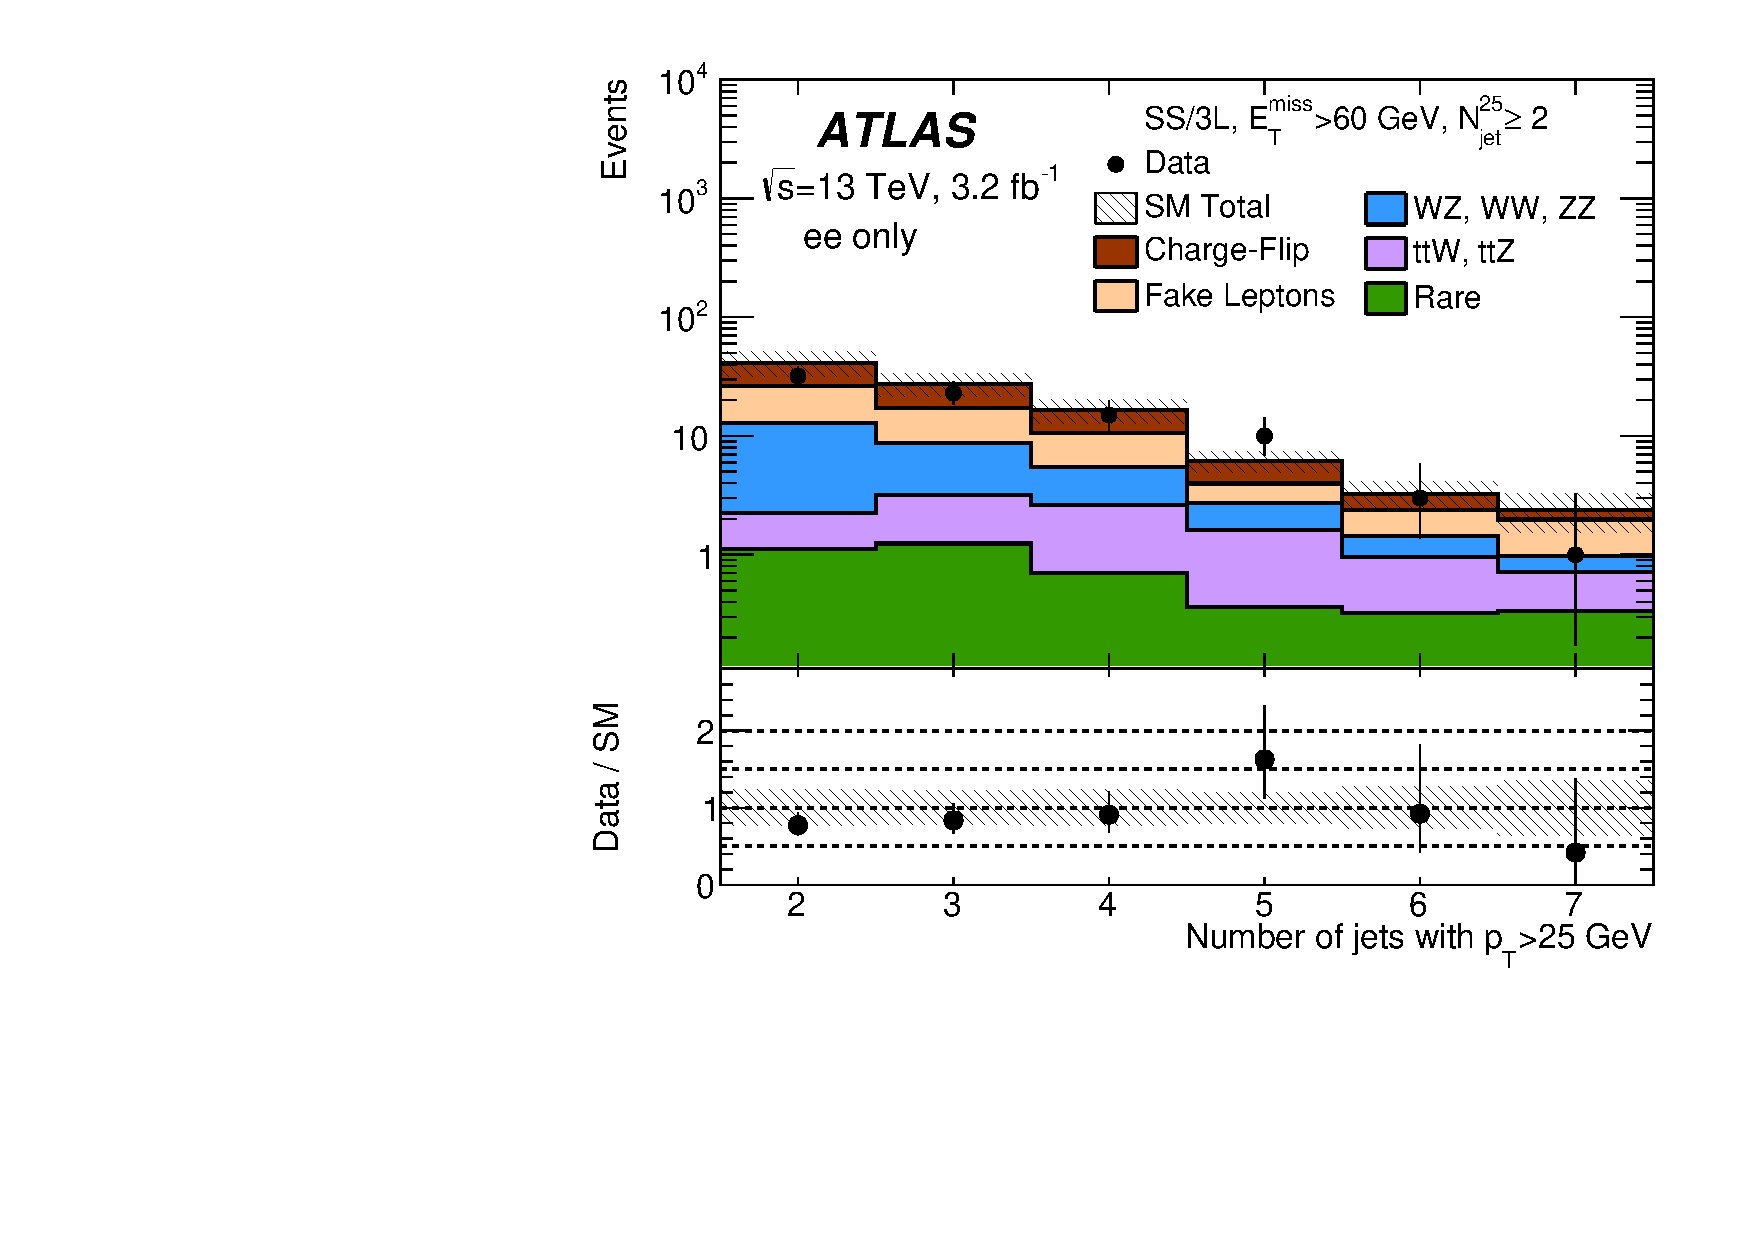
\includegraphics[width=0.45\textwidth]{CONF_EE_LEP_NJETS25.pdf}
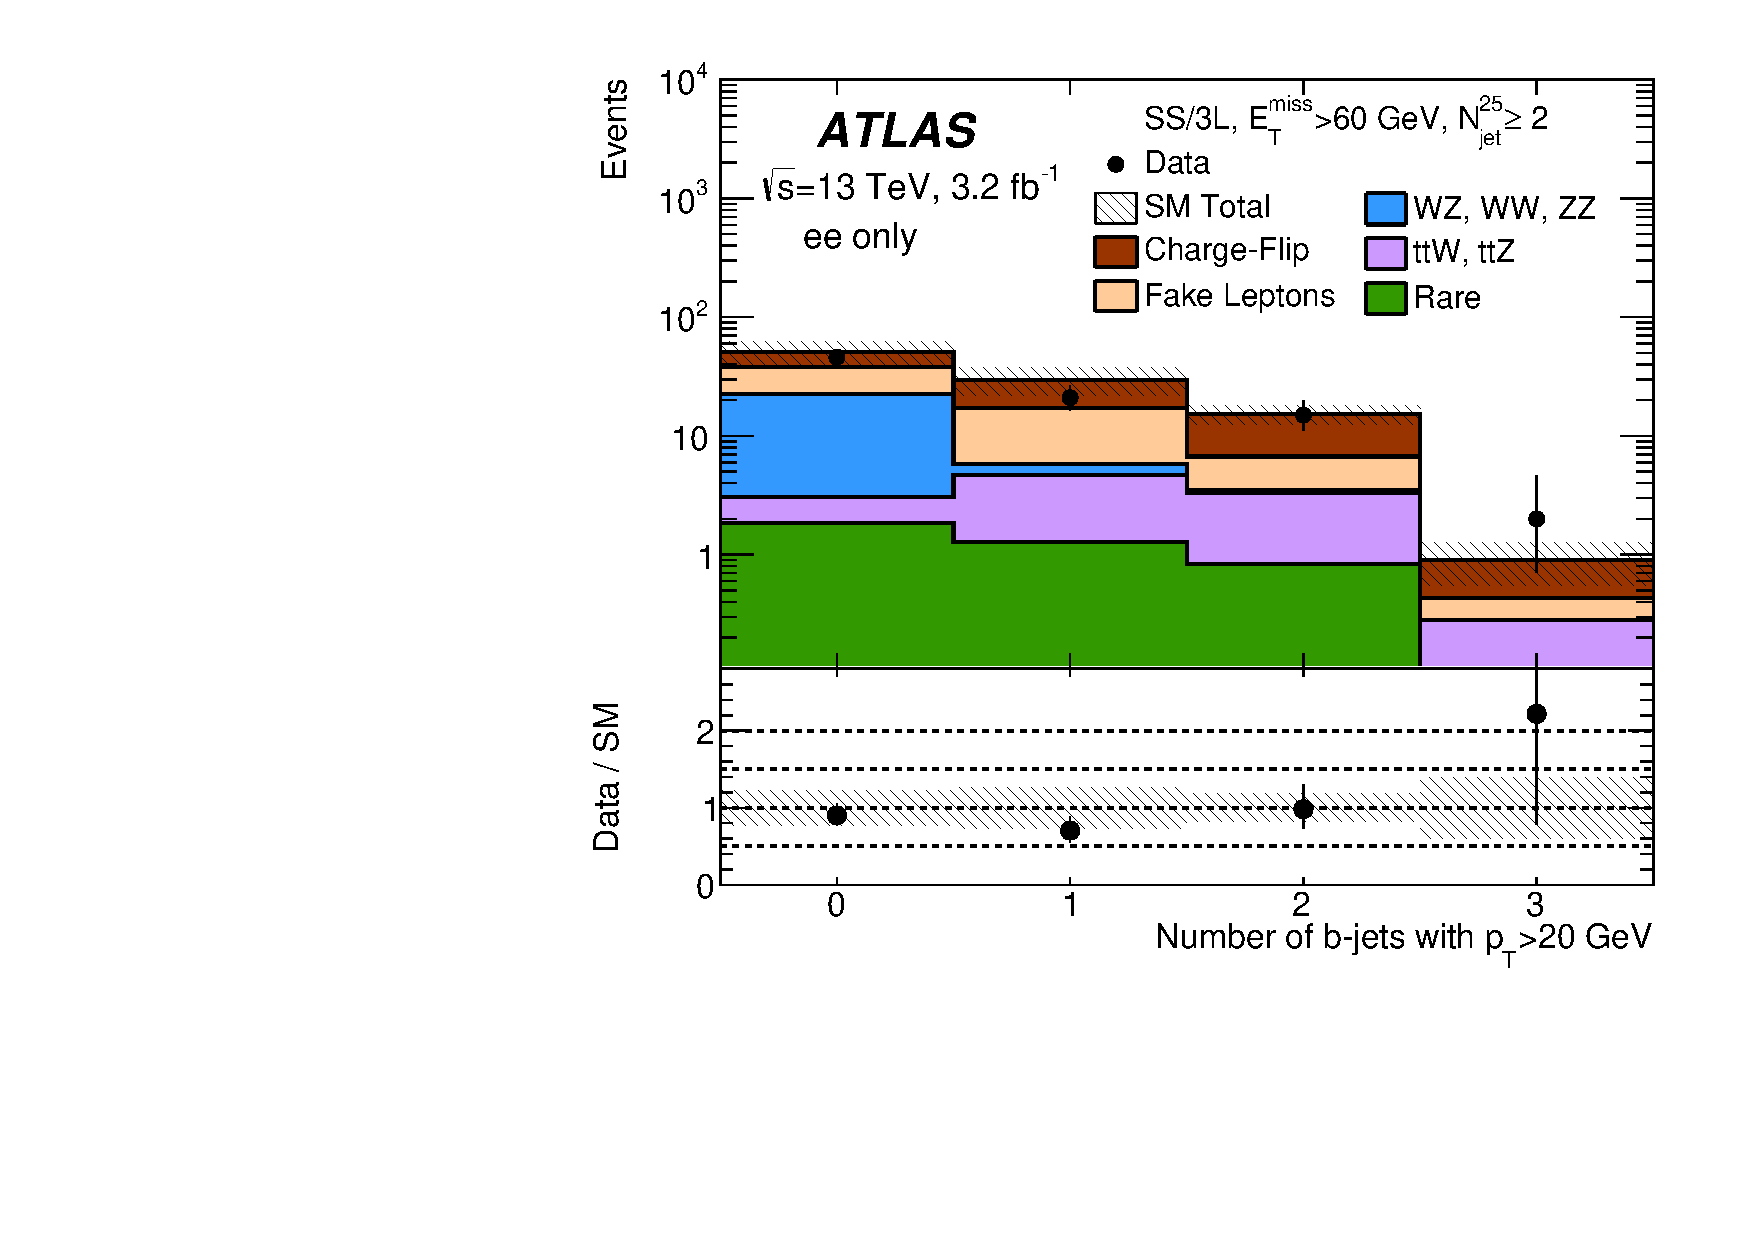
\includegraphics[width=0.45\textwidth]{CONF_EE_LEP_NBJETS20.pdf}\\
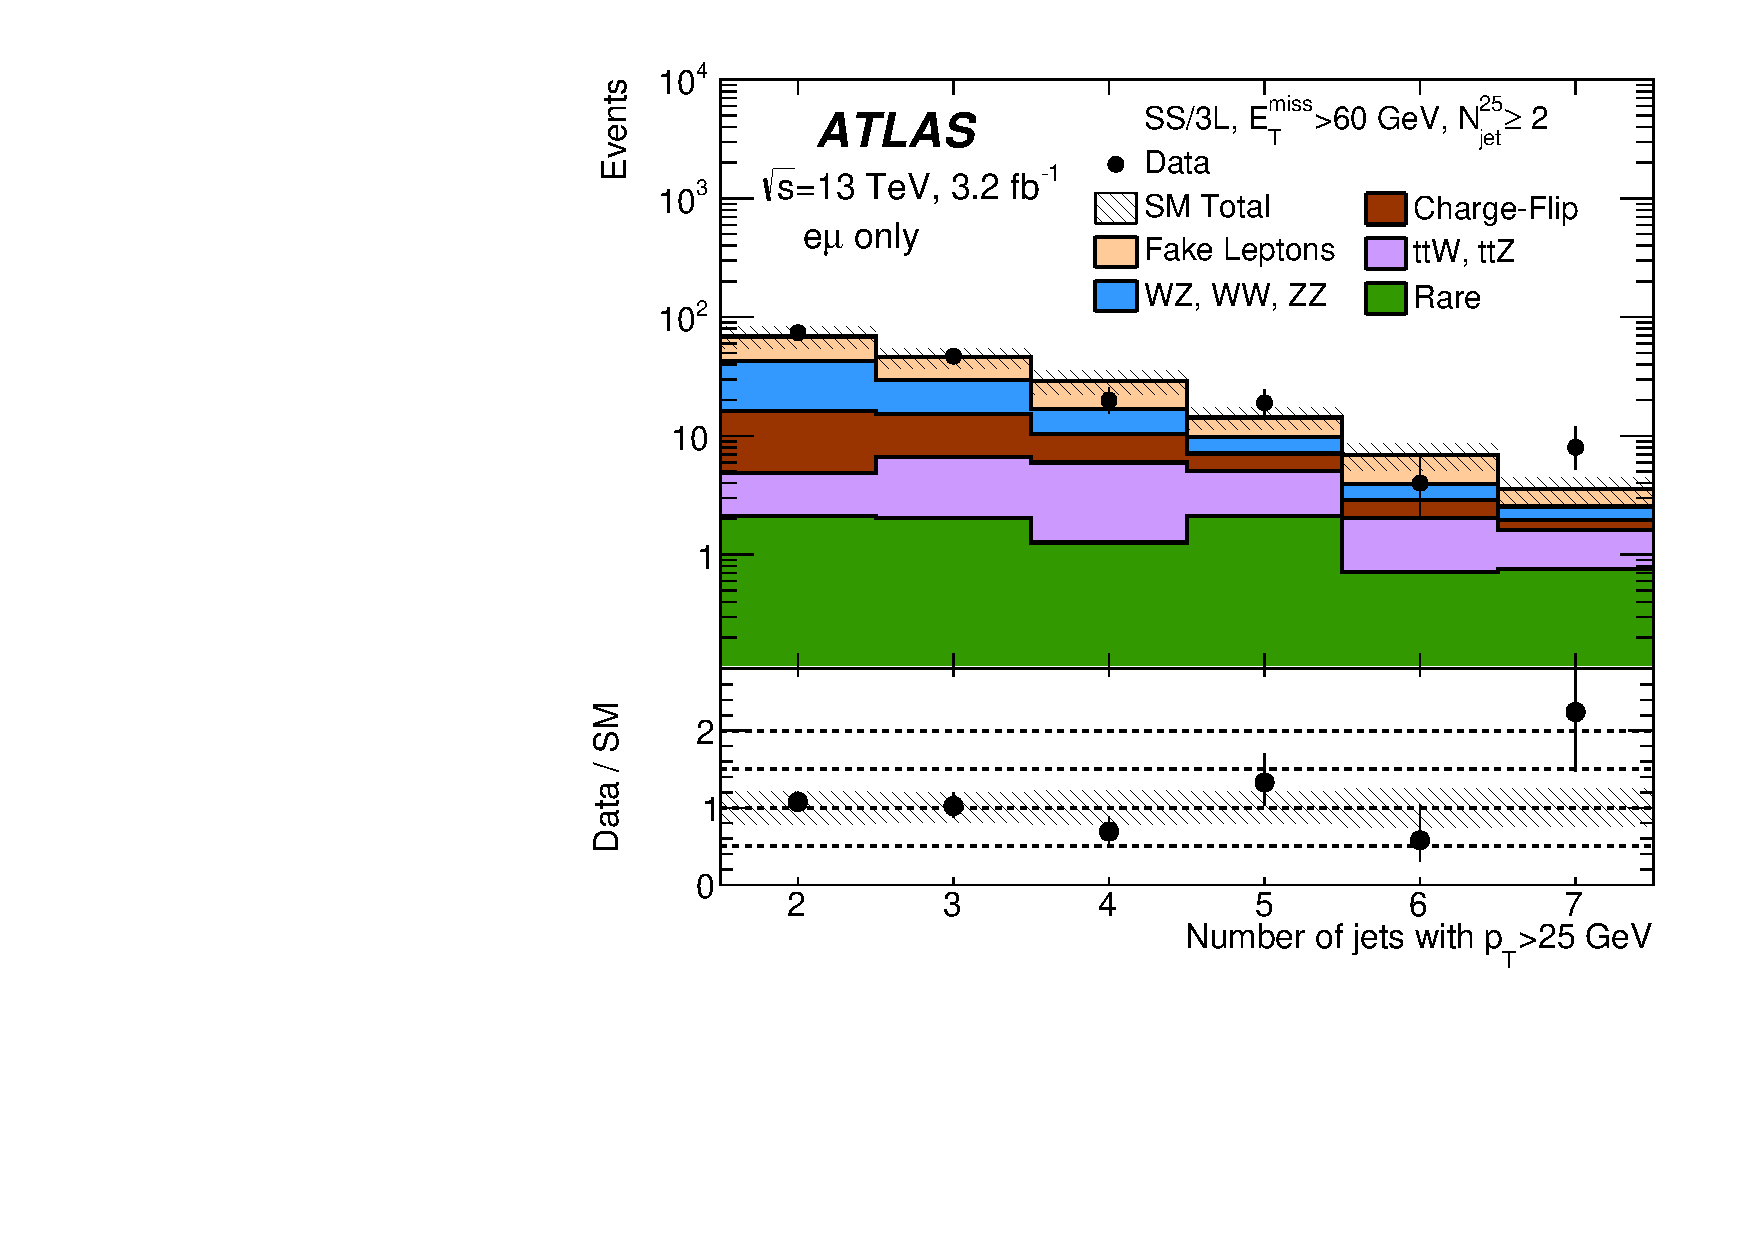
\includegraphics[width=0.45\textwidth]{CONF_EM_LEP_NJETS25.pdf}
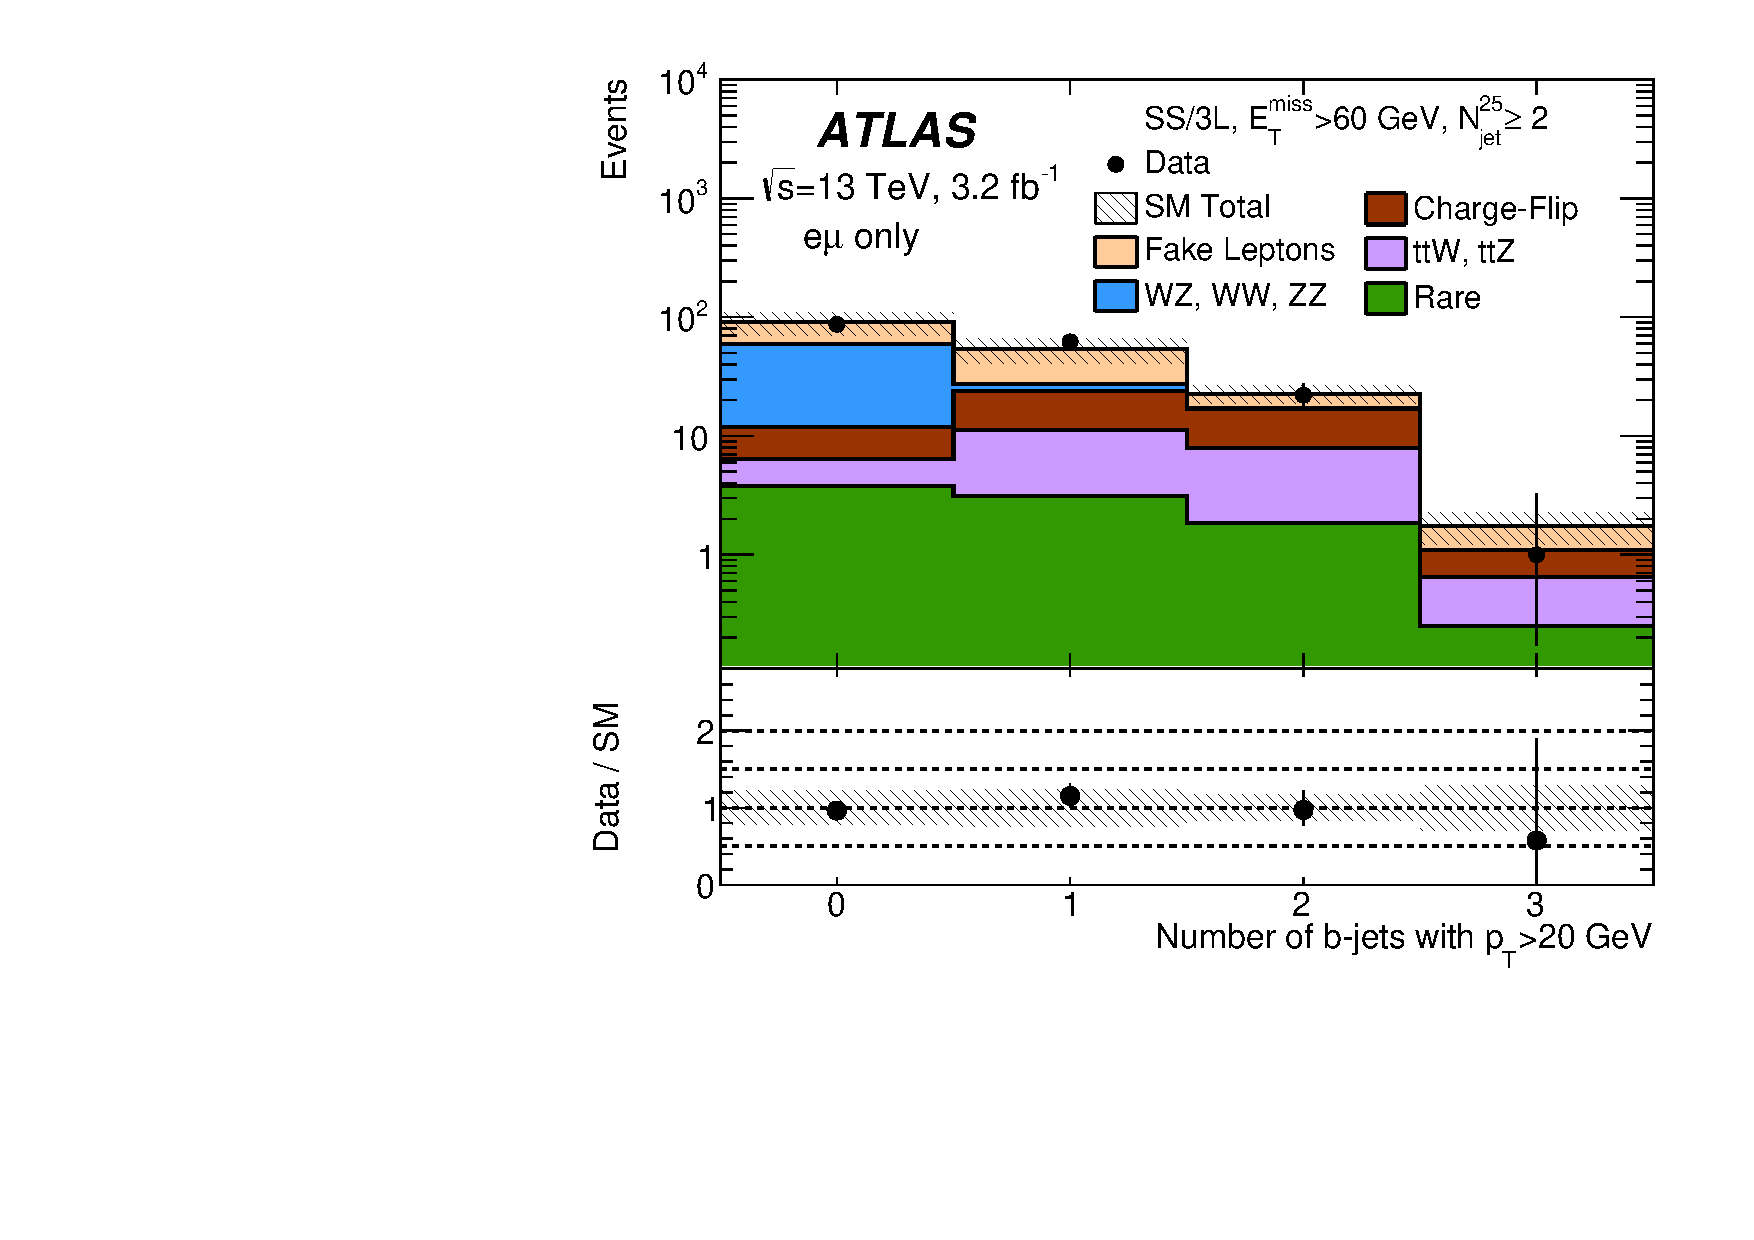
\includegraphics[width=0.45\textwidth]{CONF_EM_LEP_NBJETS20.pdf}\\
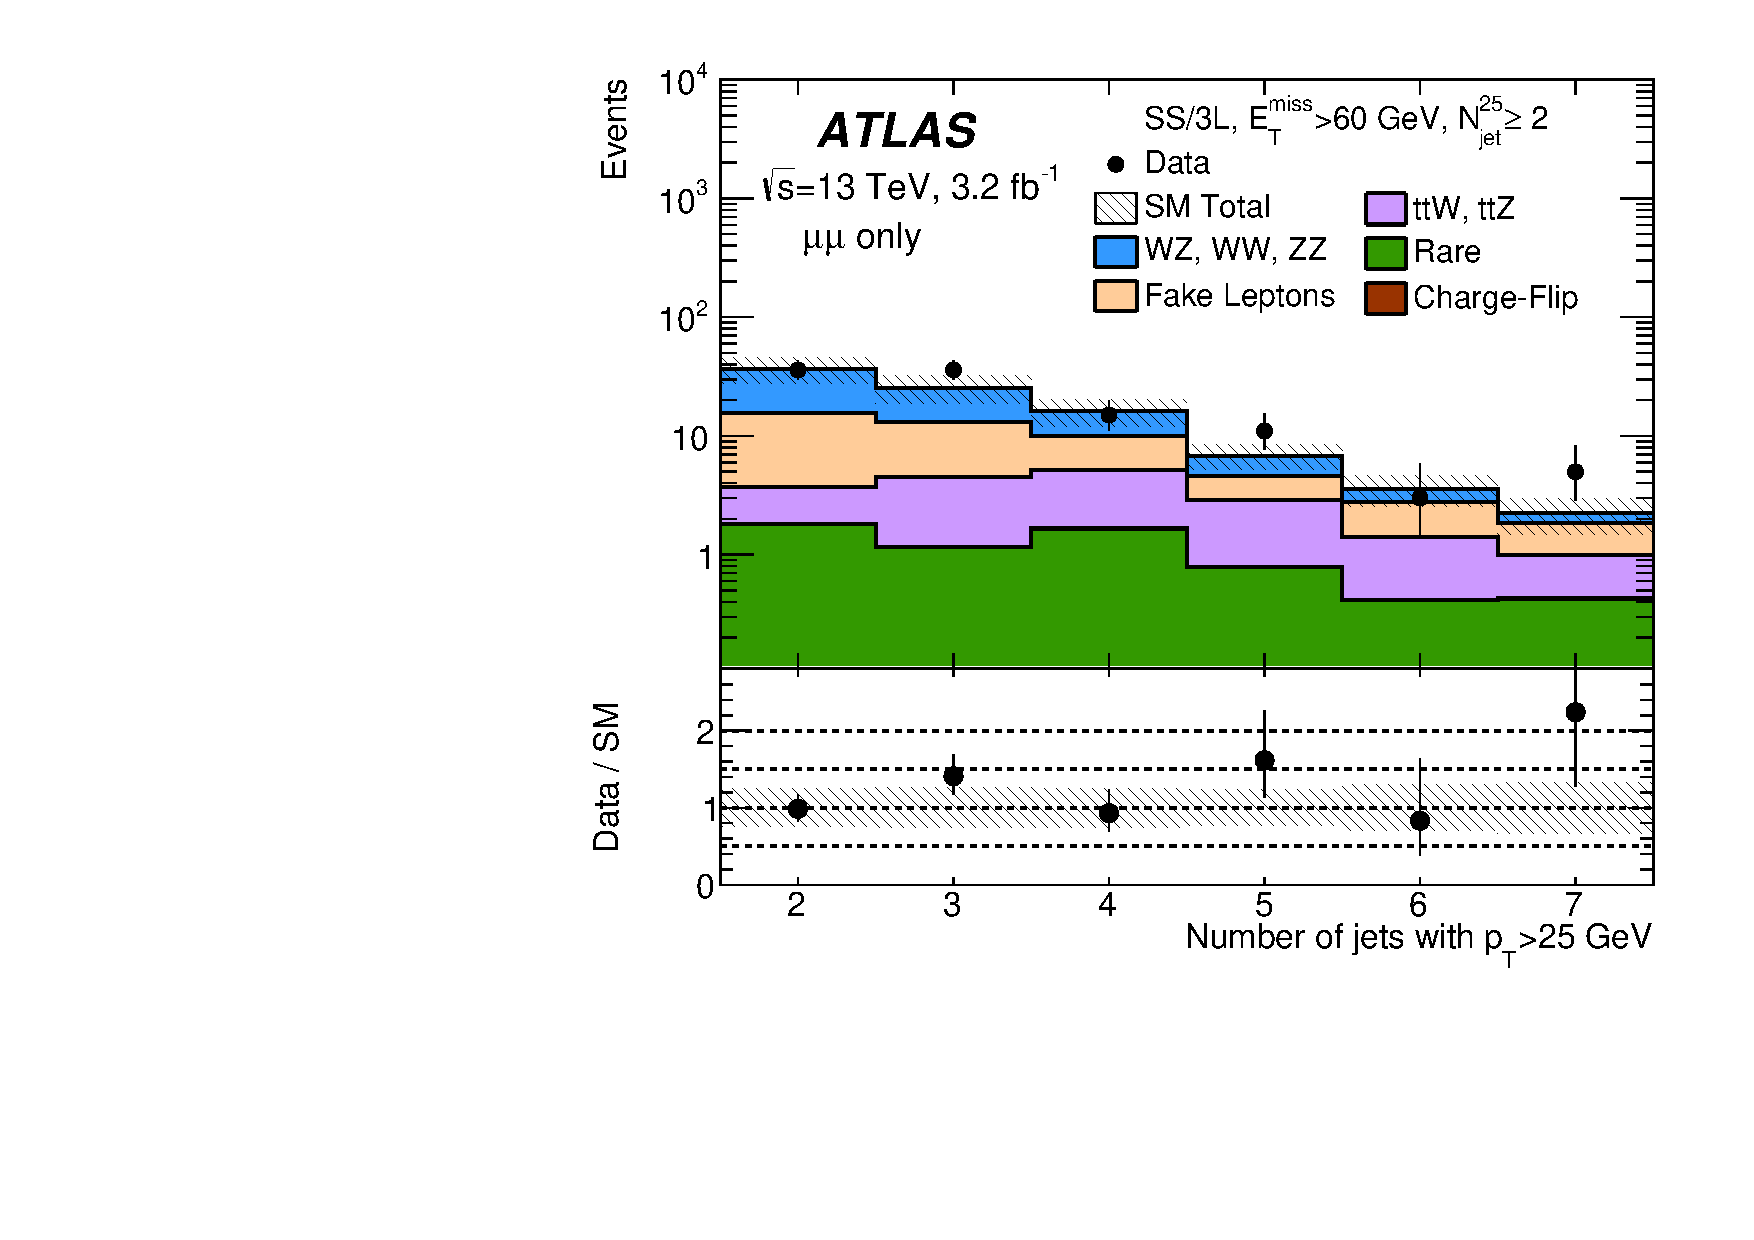
\includegraphics[width=0.45\textwidth]{CONF_MM_LEP_NJETS25.pdf}
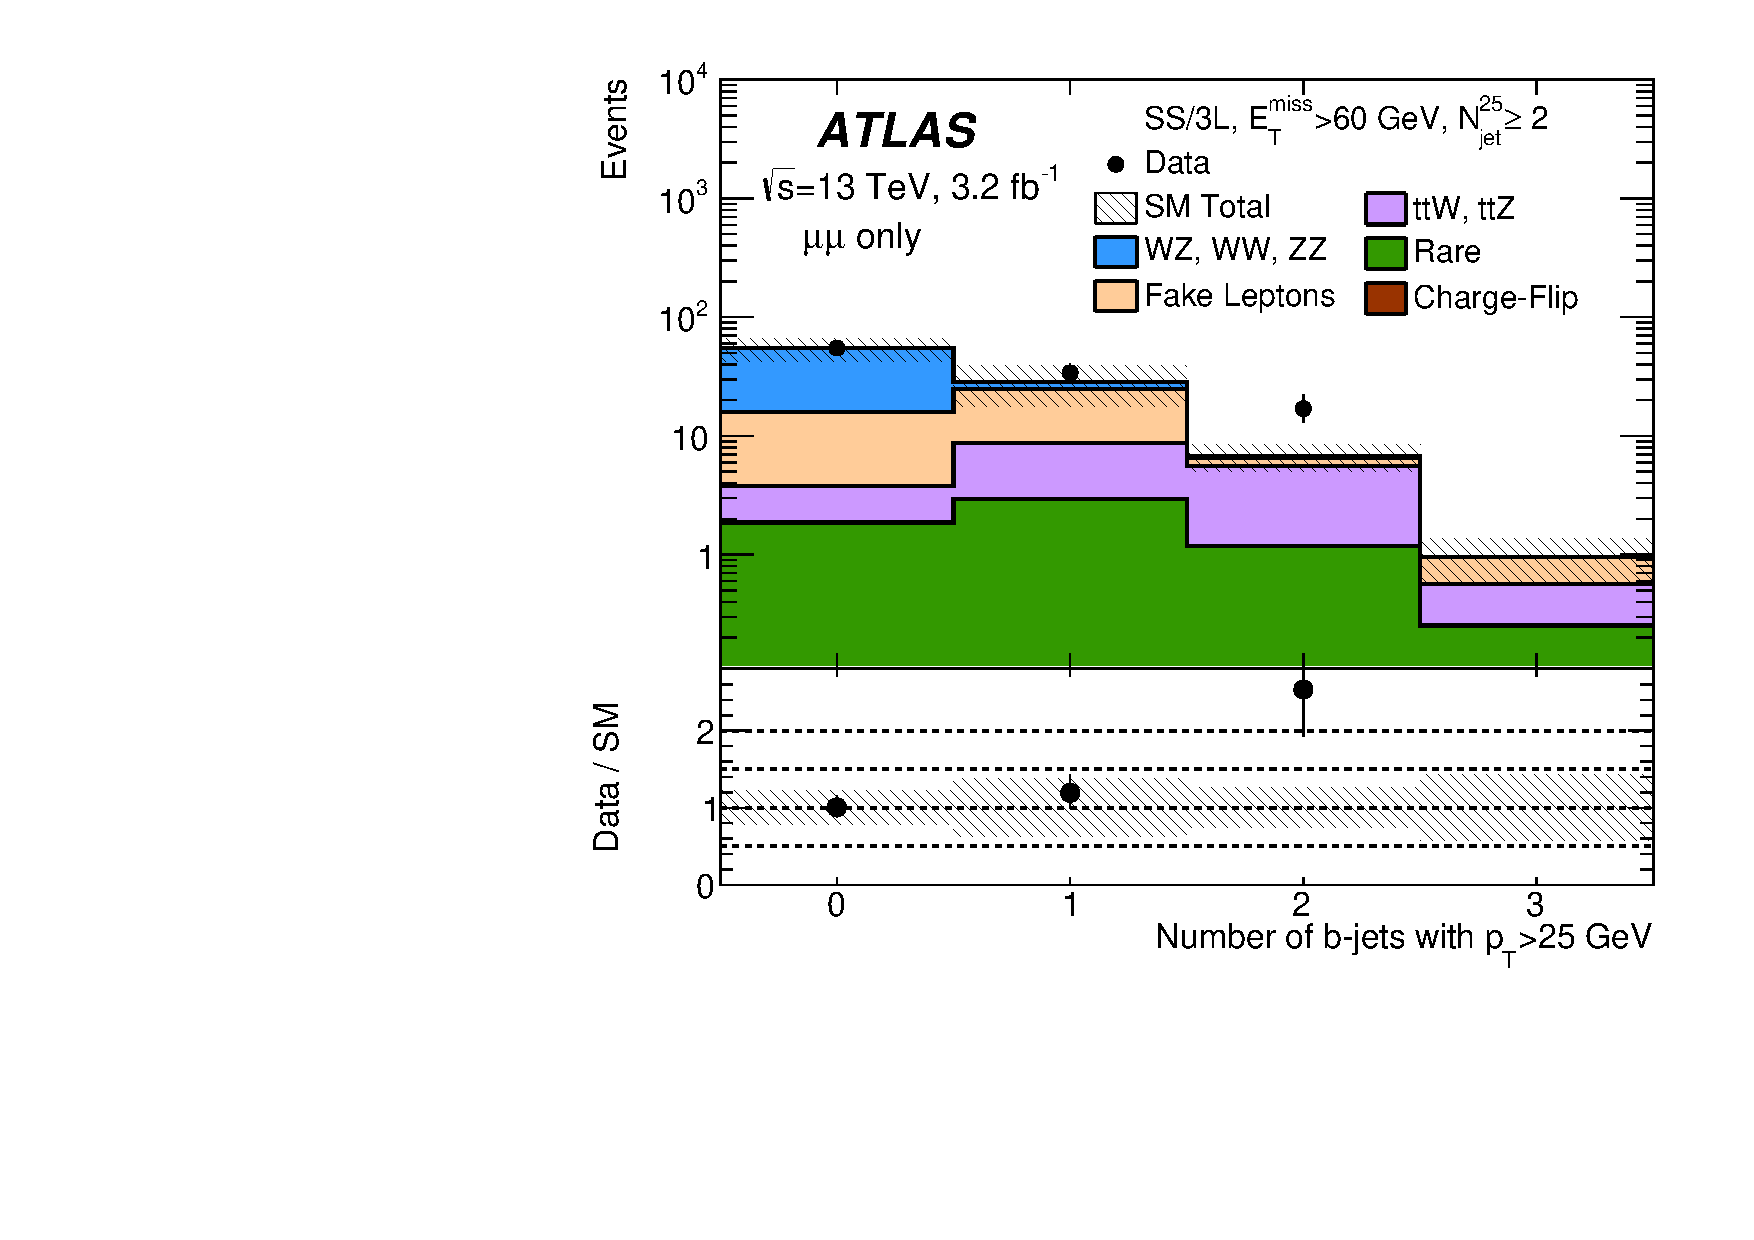
\includegraphics[width=0.45\textwidth]{CONF_MM_LEP_NBJETS20.pdf}\\
\caption{Distributions of the number of jets with $\pt>25$~GeV (left) and number of $b$-jets with $\pt>20$~GeV (right) 
for events in the $ee$ (top), $e\mu$ (middle) and $\mu\mu$ channels (bottom).
The statistical uncertainties in the background prediction are included in the uncertainty band, 
as well as the theory uncertainties for the backgrounds with prompt SS/3L, 
and the full systematic uncertainties for data-driven backgrounds. 
The last bin includes overflows. 
The ``Fake leptons'' category corresponds to FNP leptons (see text), 
and the ``Rare'' category contains the contributions from associated production of $\ttbar$ with $h/WW/t/\ttbar$, 
as well as $tZ$, $Wh$, $Zh$, and triboson production. 
The lower part of the figure shows the ratio of data to the background prediction.}
\label{fig:Validation_plots_CH} 
\end{figure} 

\begin{figure}[tbh!]
\centering
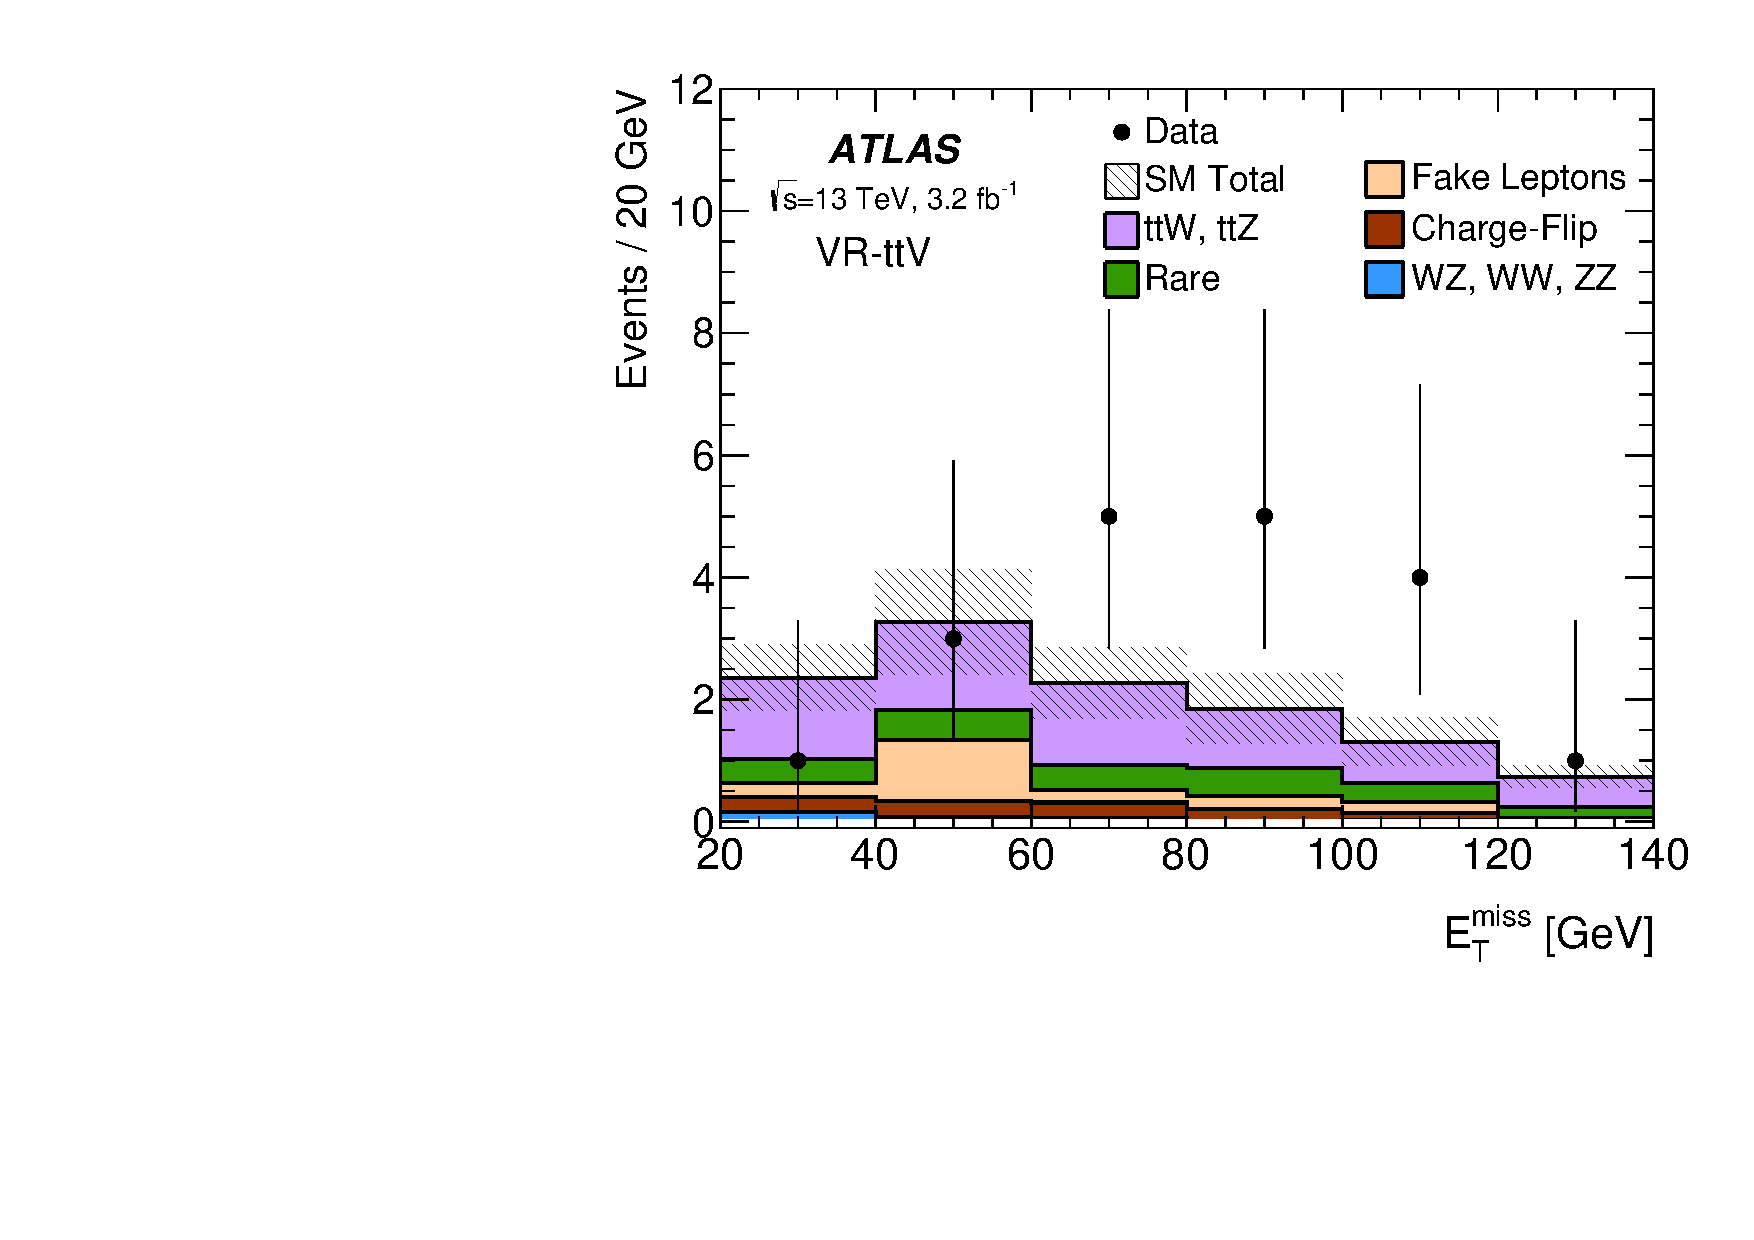
\includegraphics[width=0.45\textwidth]{CONF_ttV2bInclVR_met.pdf}
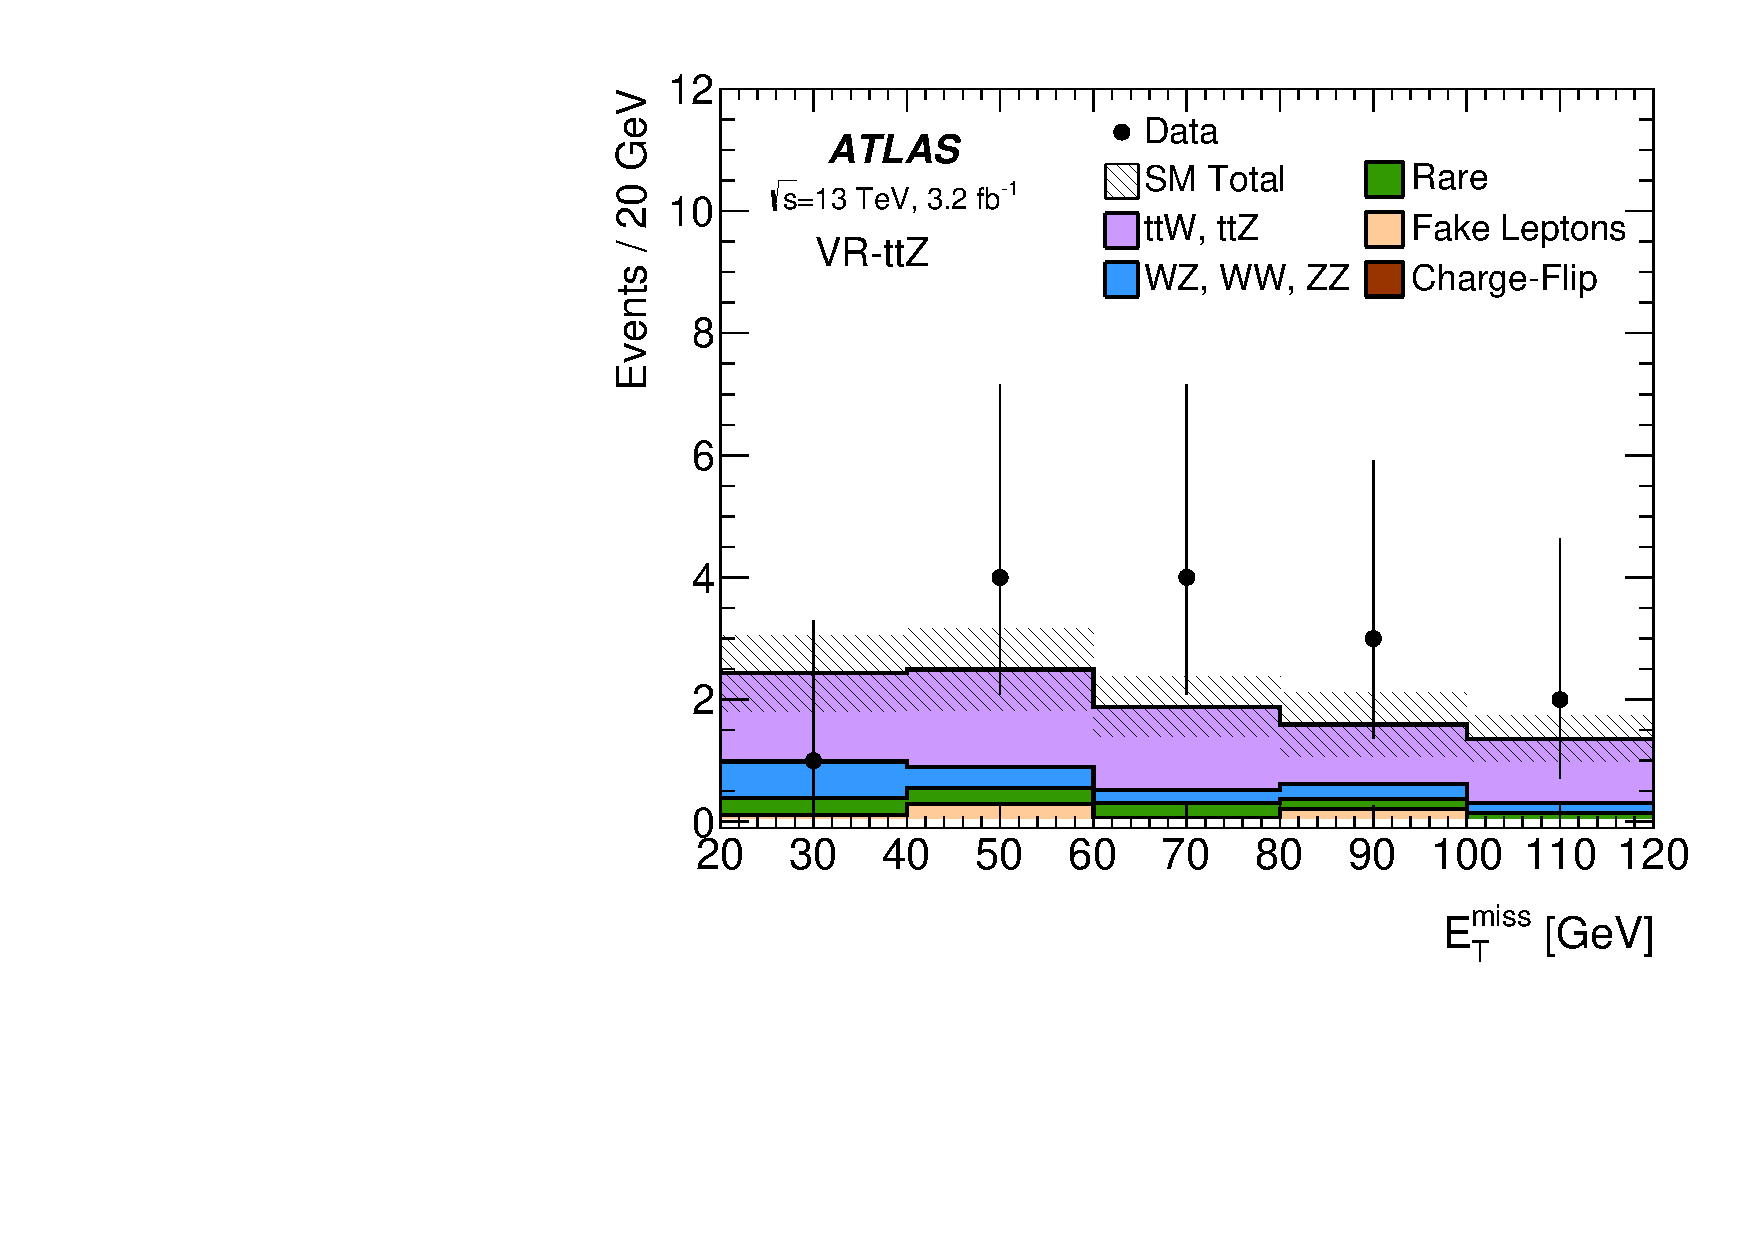
\includegraphics[width=0.45\textwidth]{CONF_ttZ1bInclVR_met.pdf}\\
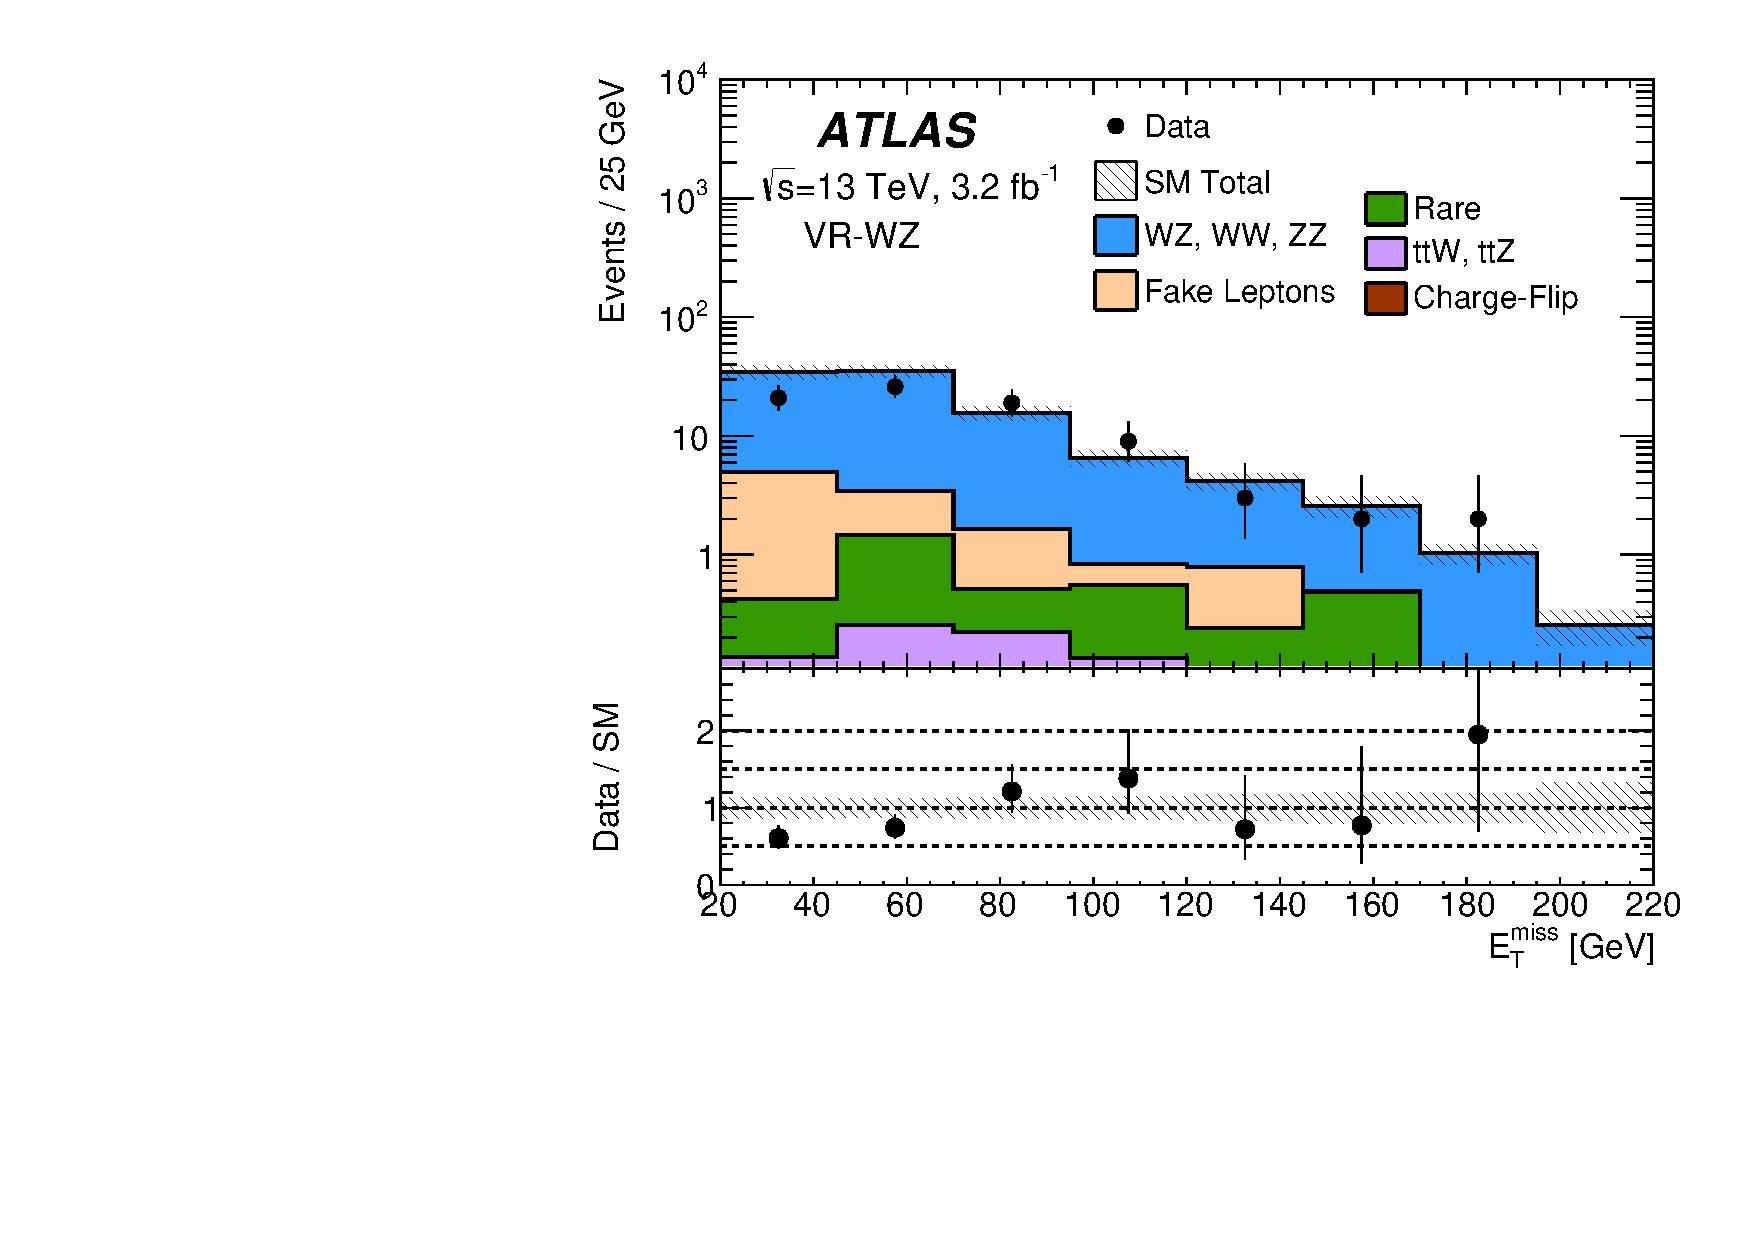
\includegraphics[width=0.45\textwidth]{CONF_WZVR_met.pdf}
\caption{Missing transverse momentum distribution in VR-ttV (top left), VR-ttZ (top right) and VR-WZ (bottom). 
The statistical uncertainties in the background prediction are included in the uncertainty band, 
as well as the theory uncertainties for the backgrounds with prompt SS/3L, 
and the full systematic uncertainties for data-driven backgrounds. 
The last bin includes overflows. 
The ``Fake leptons'' category corresponds to FNP leptons (see text), 
and the ``Rare'' category contains the contributions from associated production of $\ttbar$ with $h/WW/t/\ttbar$, 
as well as $tZ$, $Wh$, $Zh$, and triboson production. 
When shown, the lower part of the figure shows the ratio of data to the background prediction.}
\label{fig:VR_plots_Aux} 
\end{figure} 

\begin{figure}[tbh!]
\centering
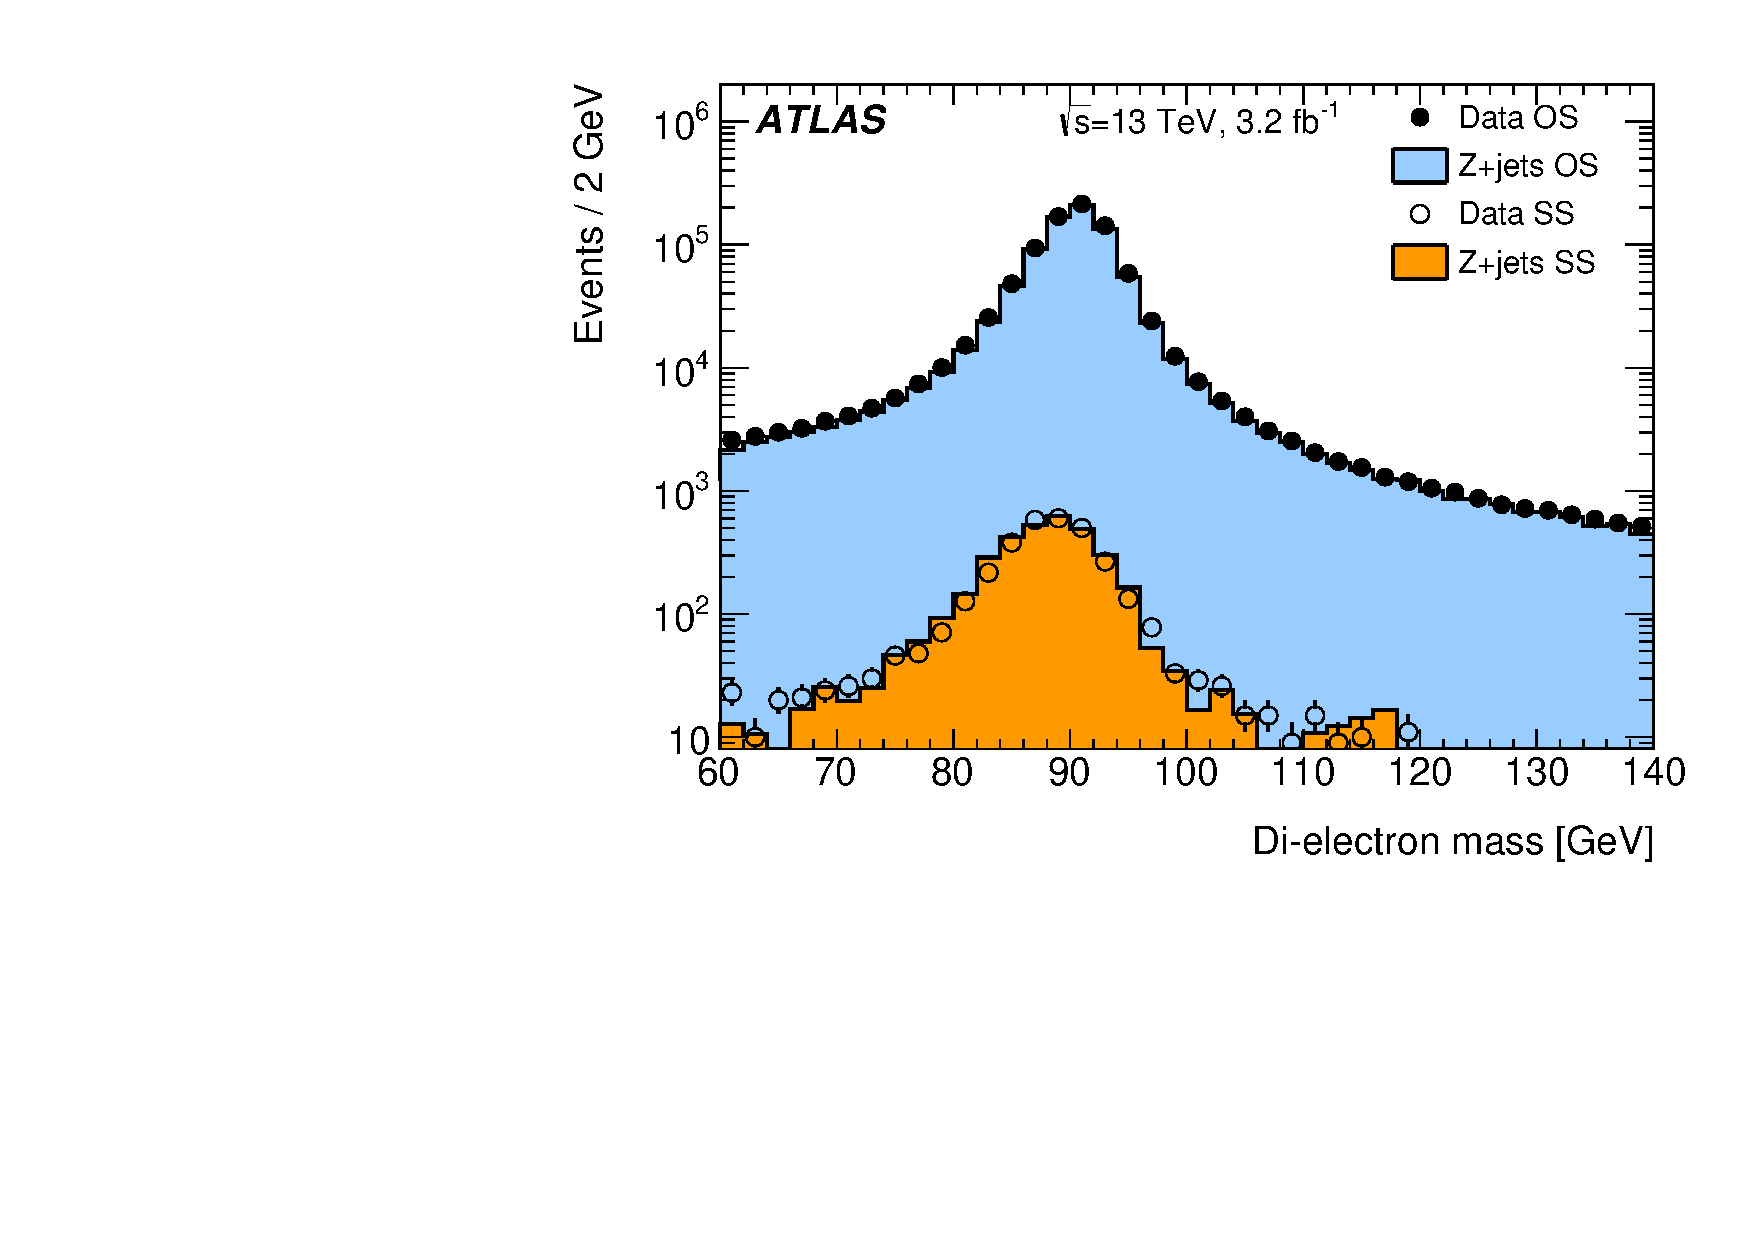
\includegraphics[width=0.55\textwidth]{ChargeFlips_3fb.pdf}
\caption{Distributions of the invariant mass for opposite-sign (OS) and same-sign (SS) dielectron pairs. 
Data are shown with full (open) circles for OS (SS) dielectron pairs including statistical uncertainty, 
and are compared with the expected contribution from simulated $Z\to ee$ events (filled areas). }
\label{fig:ChFlip} 
\end{figure} 


\begin{figure}[htb!]
\centering
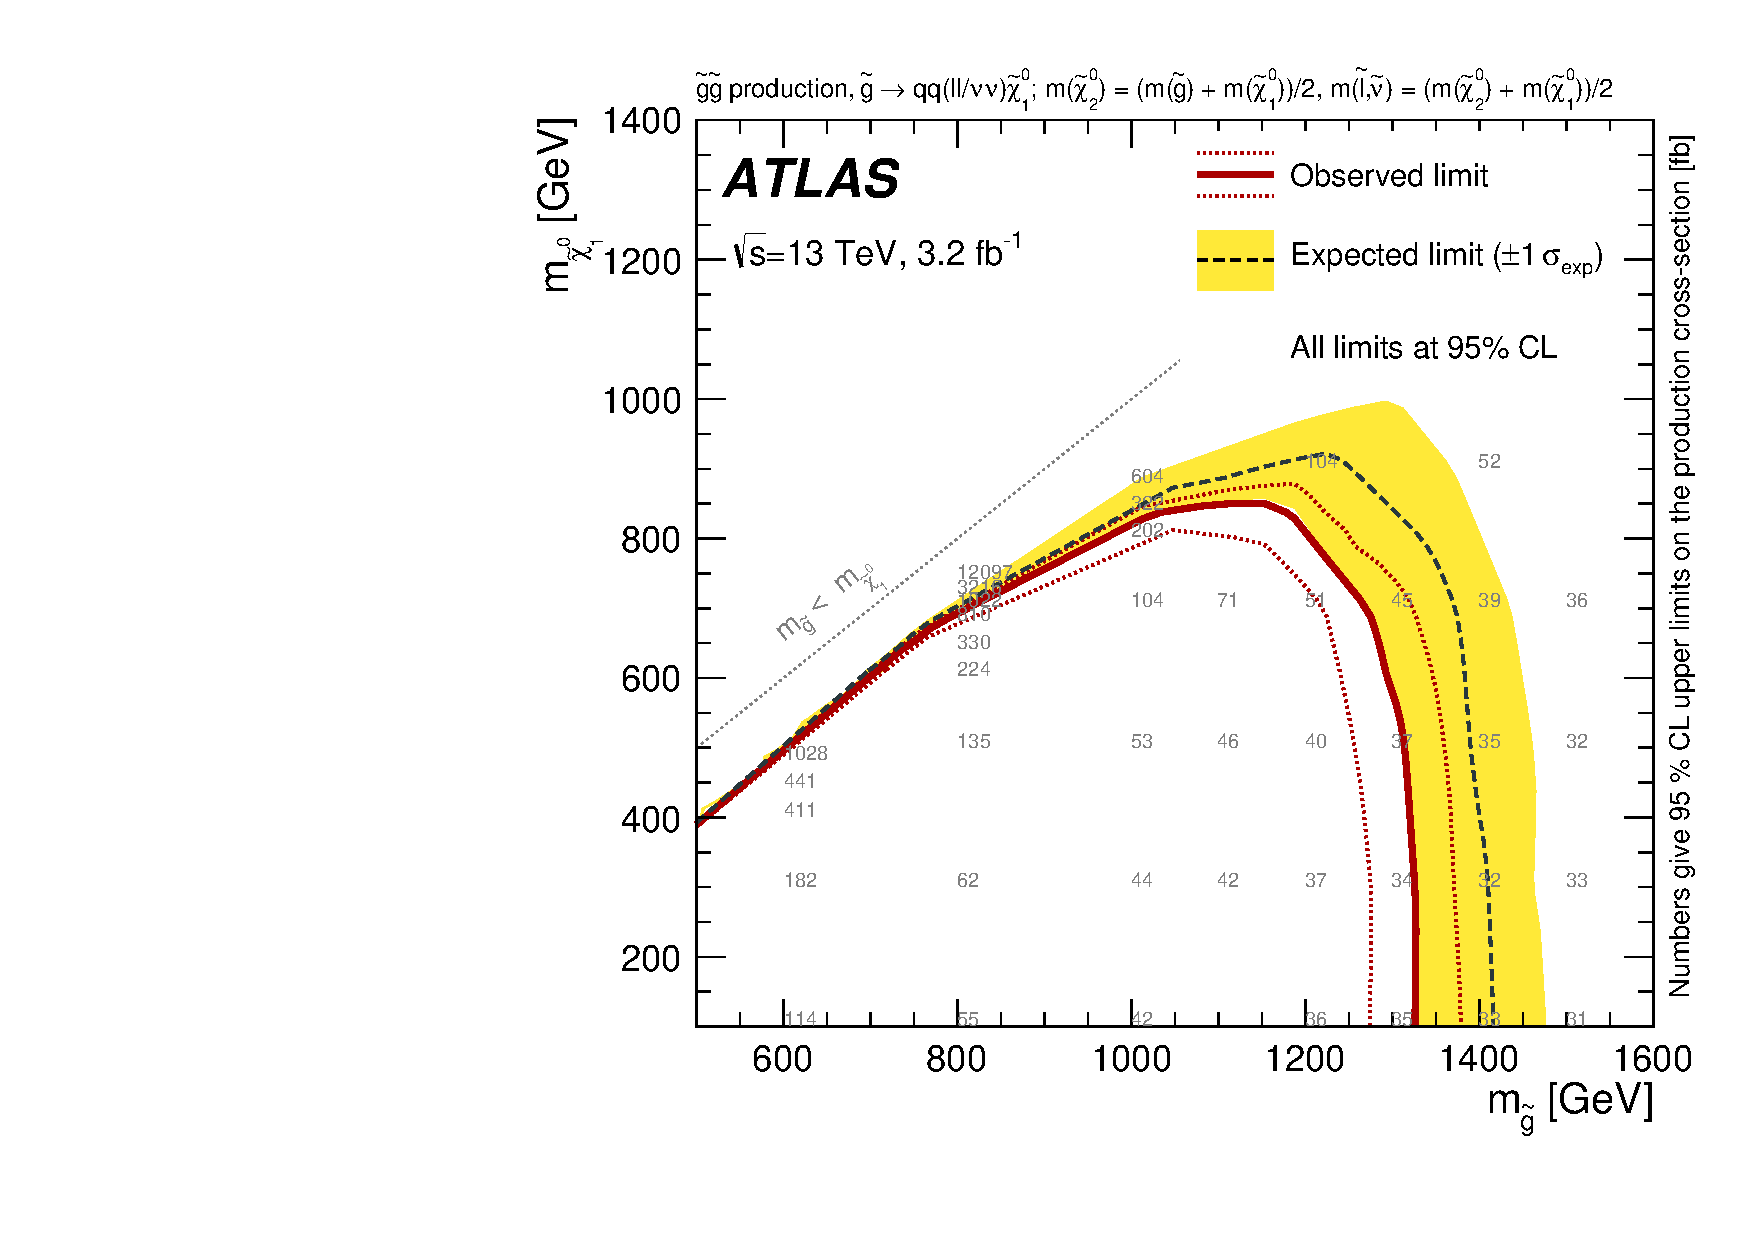
\includegraphics[width=0.48\textwidth]{exclusion2015SameSign_SR0b3jGN.pdf}
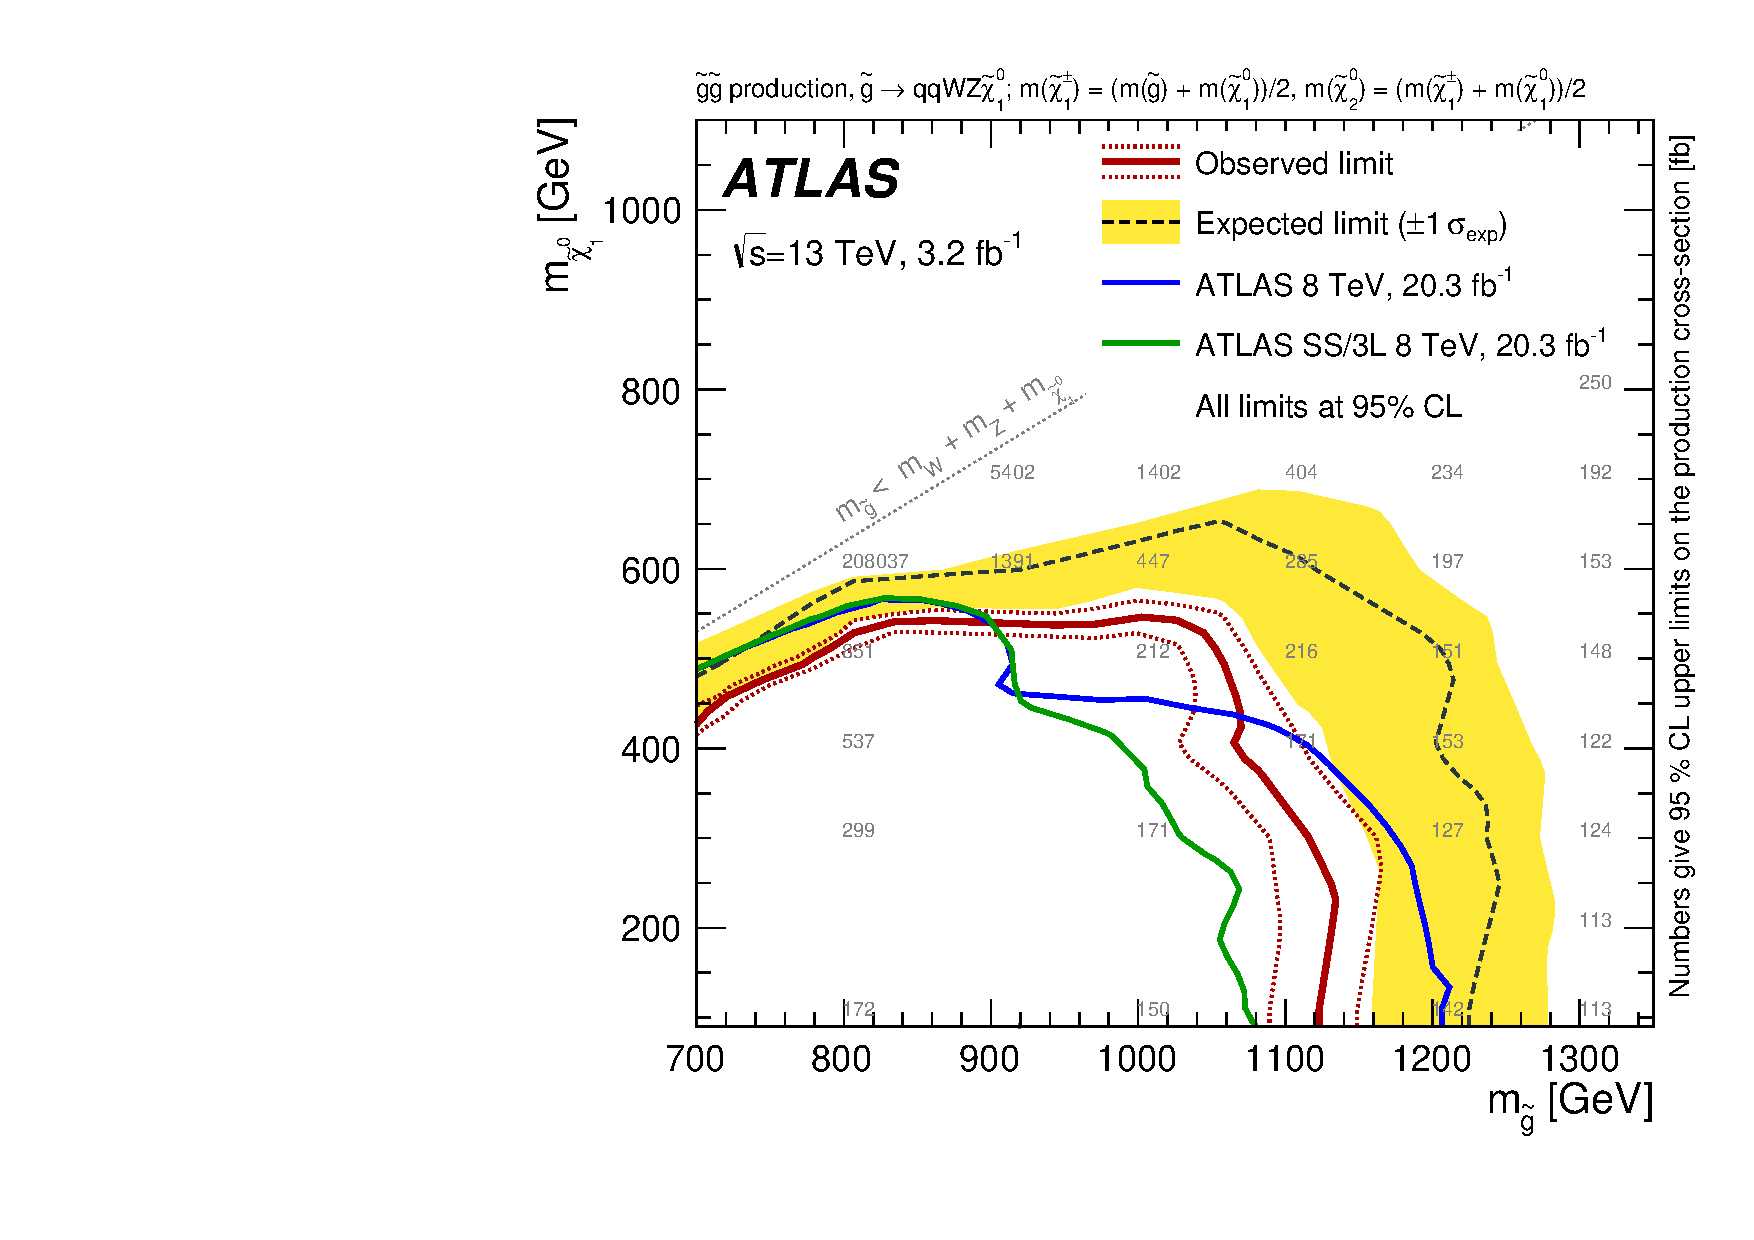
\includegraphics[width=0.48\textwidth]{exclusion2015SameSign_SR0b5jGN.pdf}\\
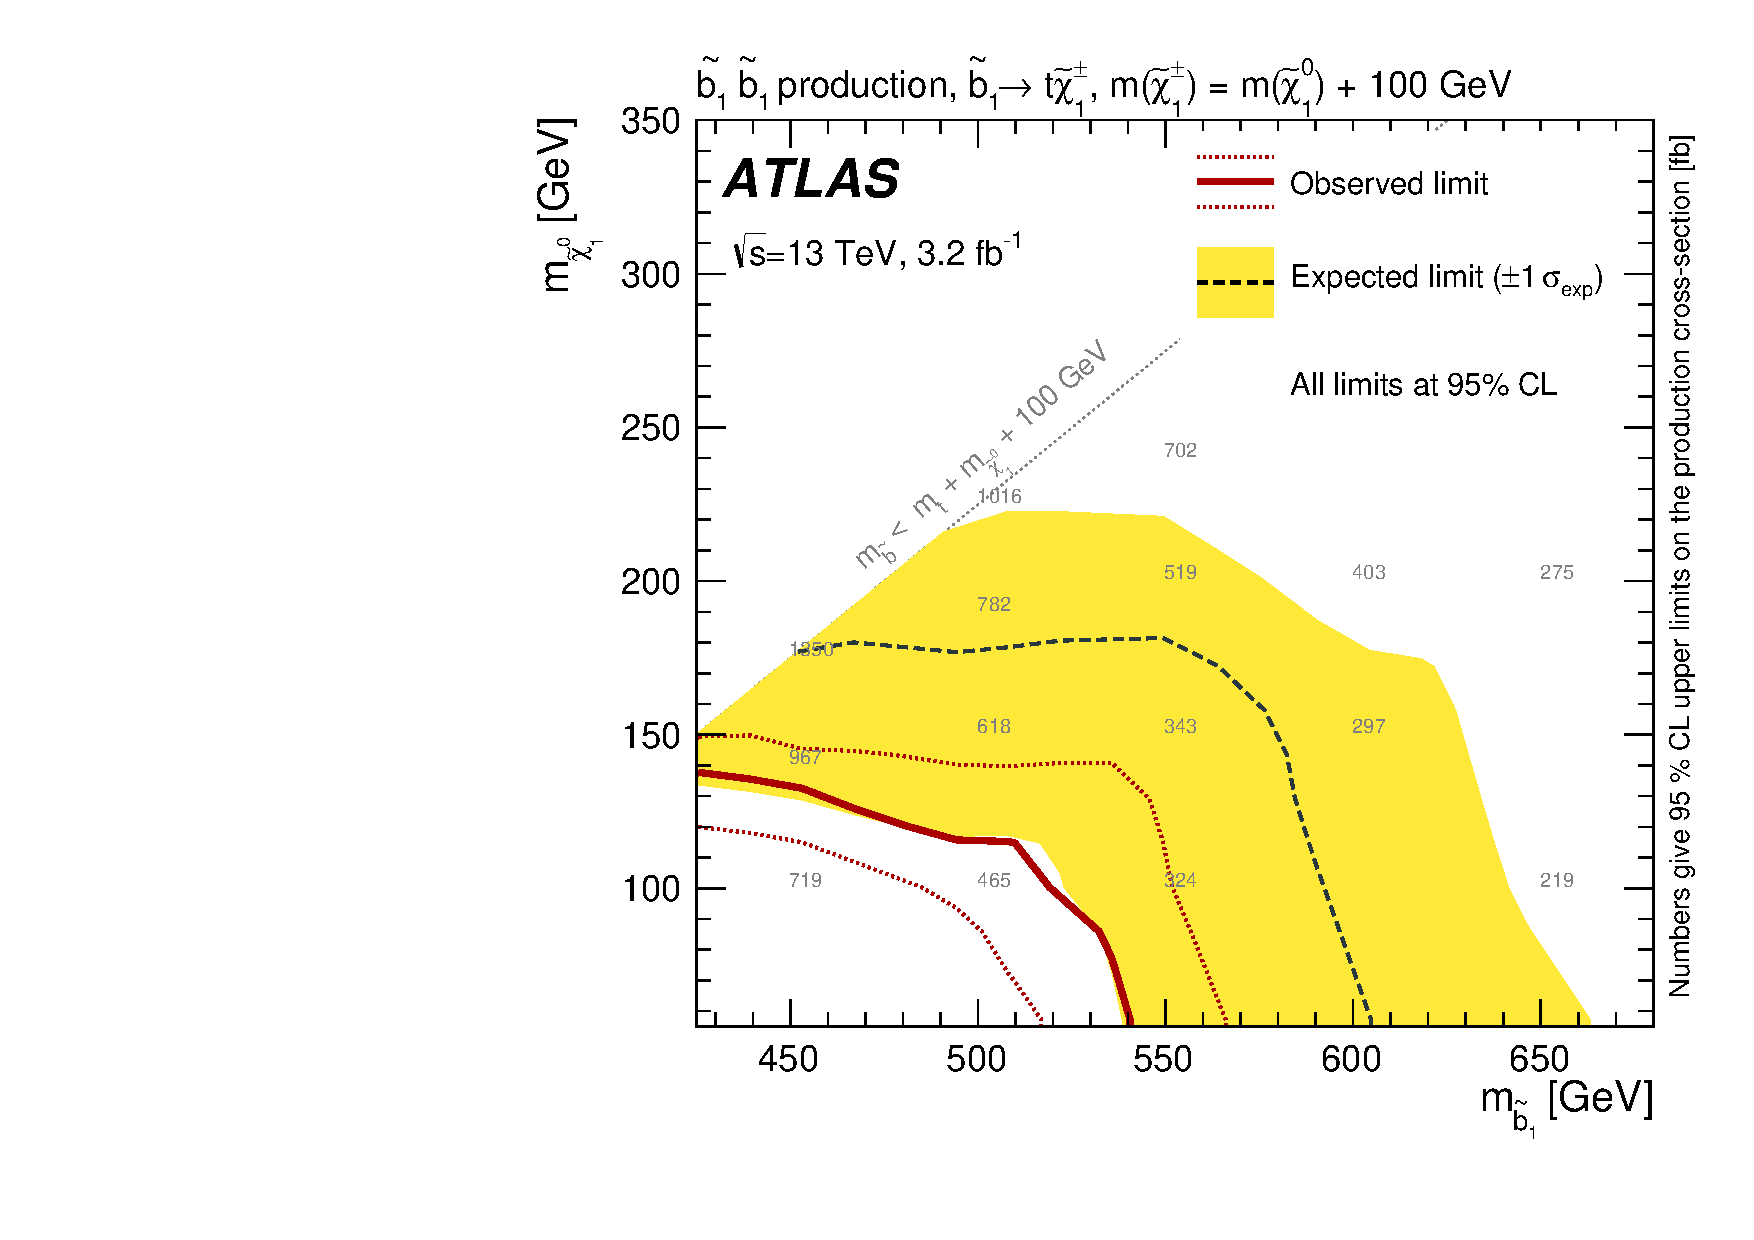
\includegraphics[width=0.48\textwidth]{exclusion2015SameSign_SR1bGN.pdf}
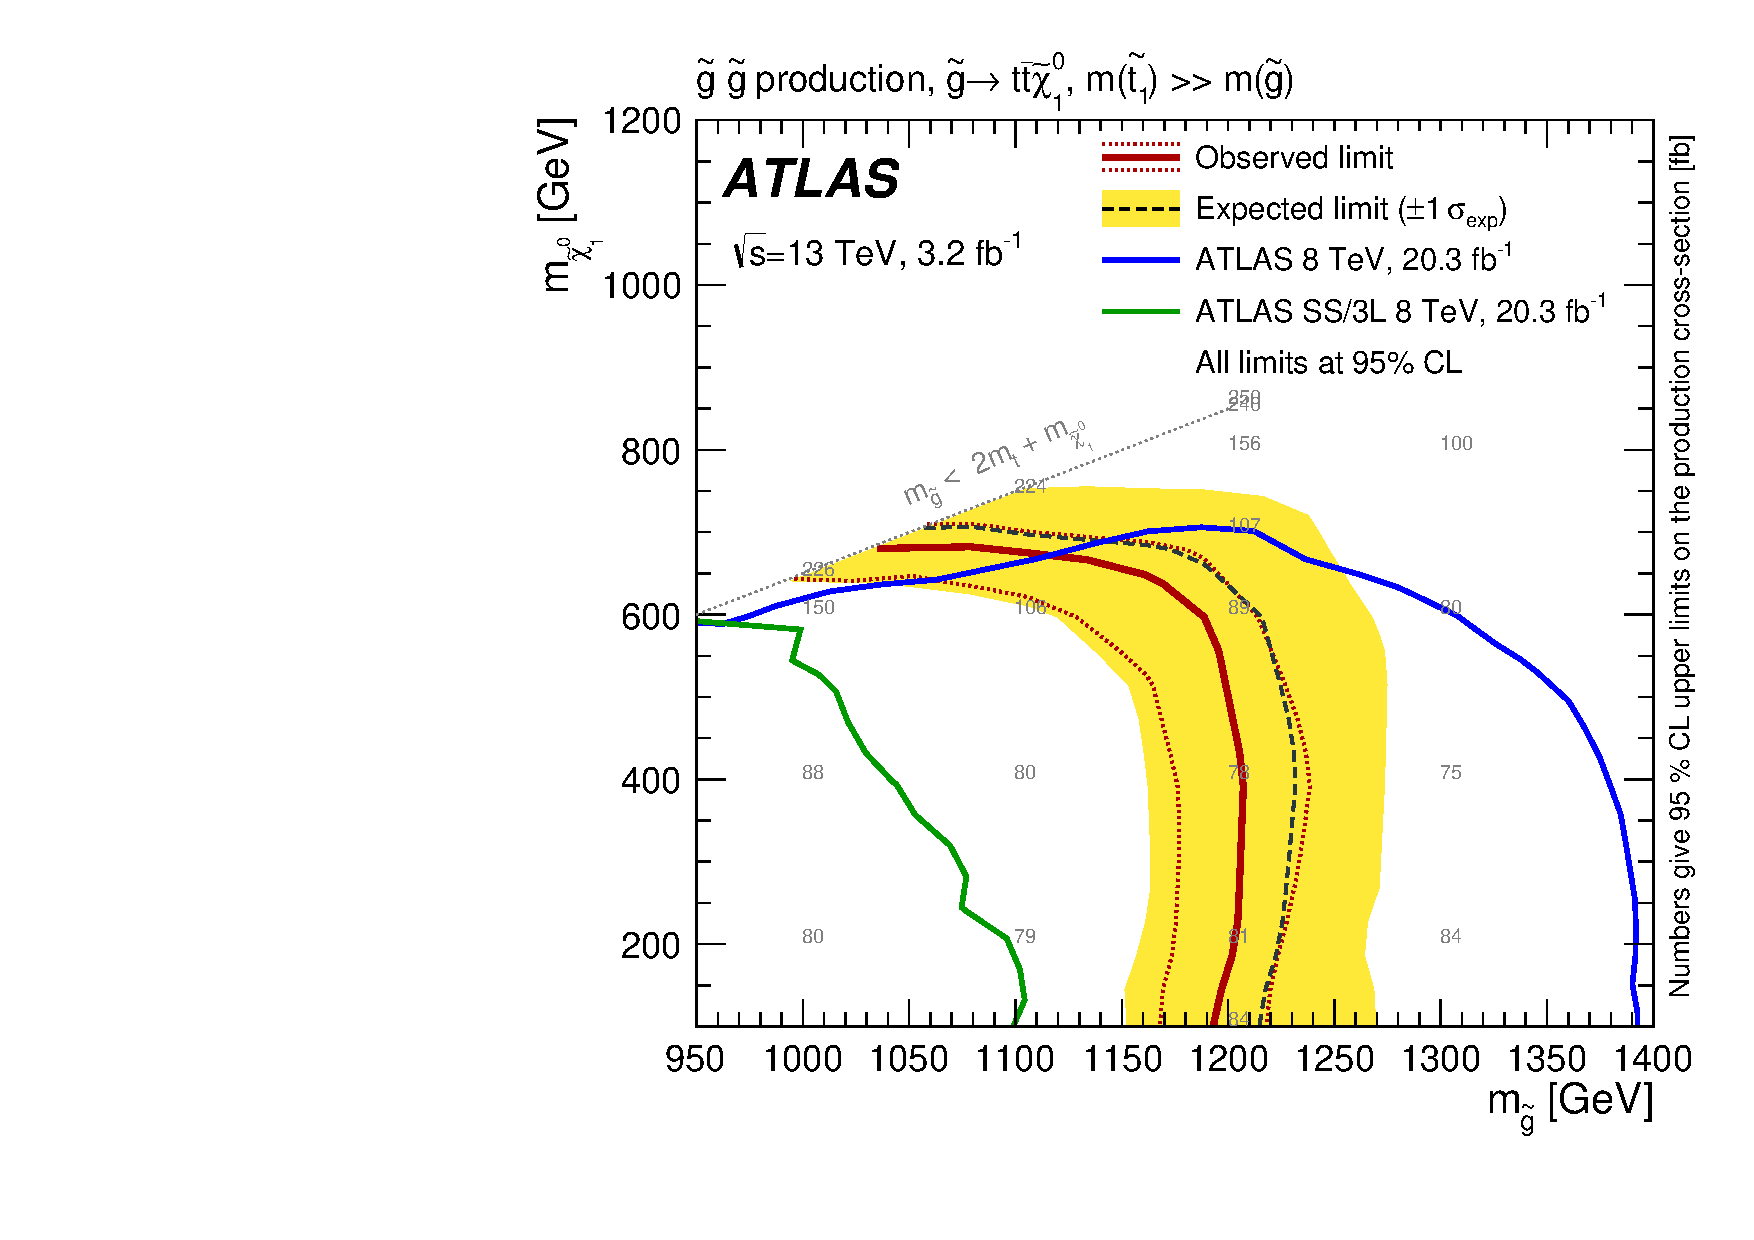
\includegraphics[width=0.48\textwidth]{exclusion2015SameSign_SR3bGN.pdf}
\caption{Observed and expected exclusion limits on the \gluino, \sbottomone and \ninoone masses 
in the context of SUSY scenarios with simplified mass spectra 
featuring $\gluino\gluino$ or $\sbottomone\sbottomonebar$ pair production with exclusive decay modes. 
The contours of the band around the expected limit are the $\pm$1$\sigma$ results, 
  including all uncertainties except theoretical uncertainties on the signal cross-section. The dotted lines around the observed
    limit illustrate the change in the observed limit as the nominal signal cross-section is scaled up and down
    by the theoretical uncertainty. All limits are computed at 95\% CL.
Results are compared with the limits obtained by previous ATLAS searches~\cite{paperSS3L,Aad:2015iea,Aad:2015pfx}.
The grey numbers show 95\% CL upper limits on cross-sections (in fb) obtained using the signal efficiency and acceptance specific to each model.}
\label{fig:Results_Limits_GN} 
\end{figure} 

\FloatBarrier

\begin{table}[htb!]
\caption{Comparison of the predicted number of background events in the validation regions using the nominal estimates obtained from data and the cross-check estimates based on MC with corrections derived in dedicated control regions. Both the statistical and systematic uncertainties are shown in the table.}
\hspace{0.5cm}
\def\arraystretch{1.1}
\label{tab:MCtemp2}
{\small
\centering
    \begin{tabular}{c c c c c c}
      \hline
     &  & VR-WW & VR-WZ & VR-ttV & VR-ttZ \\\hline 
     Fake/non-prompt & Nominal  & $0.6 \pm 0.5$ & $8 \pm 6$ & $2.1 \pm 1.4$ & $0.6\pm 1.0$ \\
      & MC based & $0.01 \pm 0.01$ & $3.4 \pm 1.8$   & $1.8 \pm 1.0$ & $0.5 \pm 0.4$ \\
      \hline
Charge-flip & Nominal & $0.26 \pm 0.05$ & $-$ & $1.14 \pm 0.15$ & $-$  \\
      & MC based      & $< 0.08$  & $-$ & $0.27 \pm 0.23$ & $-$ \\
      \hline
    \end{tabular}
}
\end{table}

\begin{table}[htb!]
\caption{Comparison of the predicted number of background events in the signal regions using the nominal estimates obtained from data and the cross-check estimates based on MC with corrections derived in dedicated control regions. Both the statistical and systematic uncertainties are shown in the table.}
\hspace{0.5cm}
\def\arraystretch{1.1}
\label{tab:MCtemp1}
{\small
\centering
    \begin{tabular}{c c c c c c}
      \hline
      &  & SR0b3j & SR0b5j & SR1b & SR3b \\
      \hline
      Fake/non-prompt leptons & Nominal & $<0.2$ & $0.05\pm 0.18$ & $0.8 \pm 0.8$ & $0.13 \pm 0.17$  \\
      & MC based & $< 0.15$ & $< 0.15$  & $2.7 \pm 1.9$ & $0.02 \pm 0.01$ \\
      \hline
      Charge-flip & Nominal  & $-$ & $0.02 \pm 0.01$ & $0.60 \pm 0.12$ & $0.19 \pm 0.06$ \\
      & MC based & $-$ & $< 0.08$   & $1.0 \pm 0.8$   & $< 0.08$ \\
      \hline
    \end{tabular}
}
\end{table}

\begin{figure}[p]
\centering
\begin{subfigure}[t]{0.42\textwidth}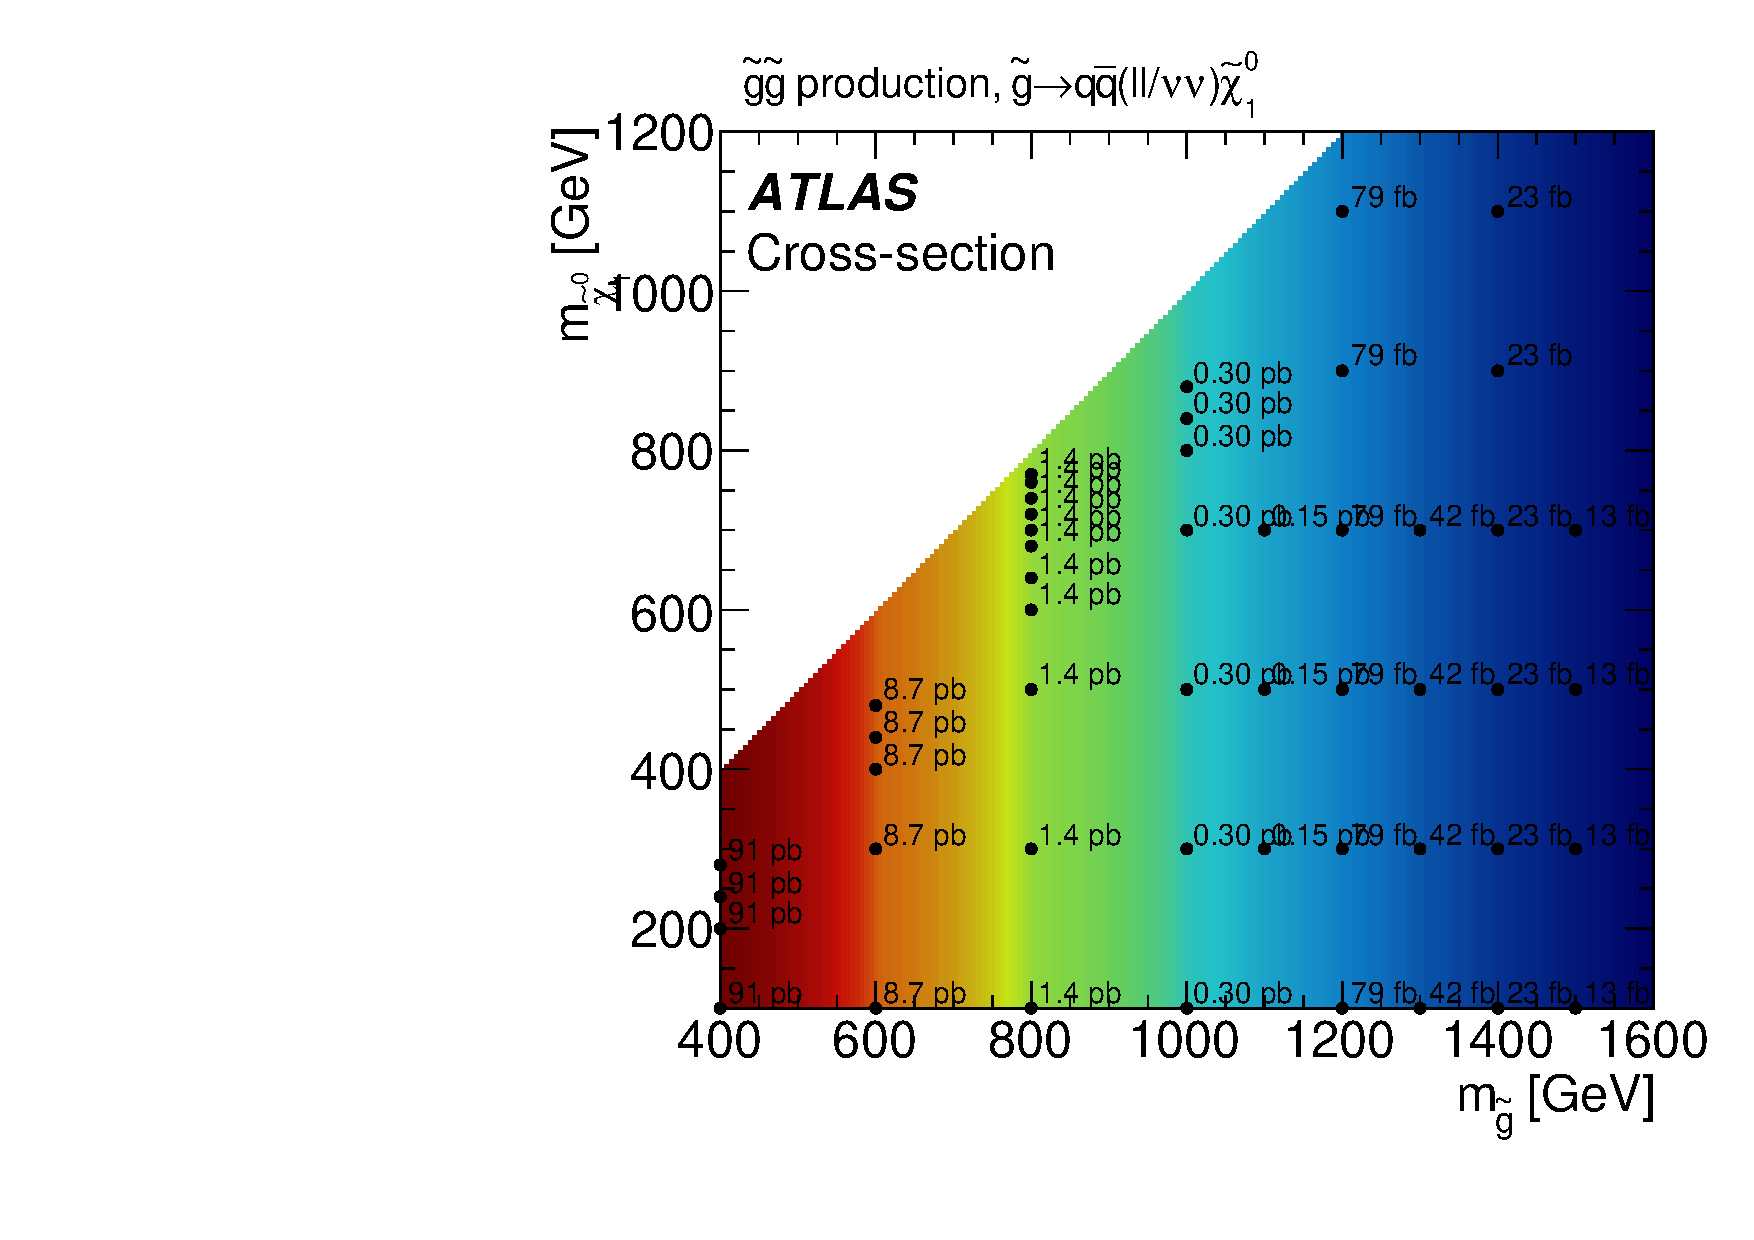
\includegraphics[width=\textwidth]{HEPDATA/xsection_SR0b3j.pdf}
\caption{}\label{fig:hepdata_SR0b3j_xsection}\end{subfigure}
\begin{subfigure}[t]{0.42\textwidth}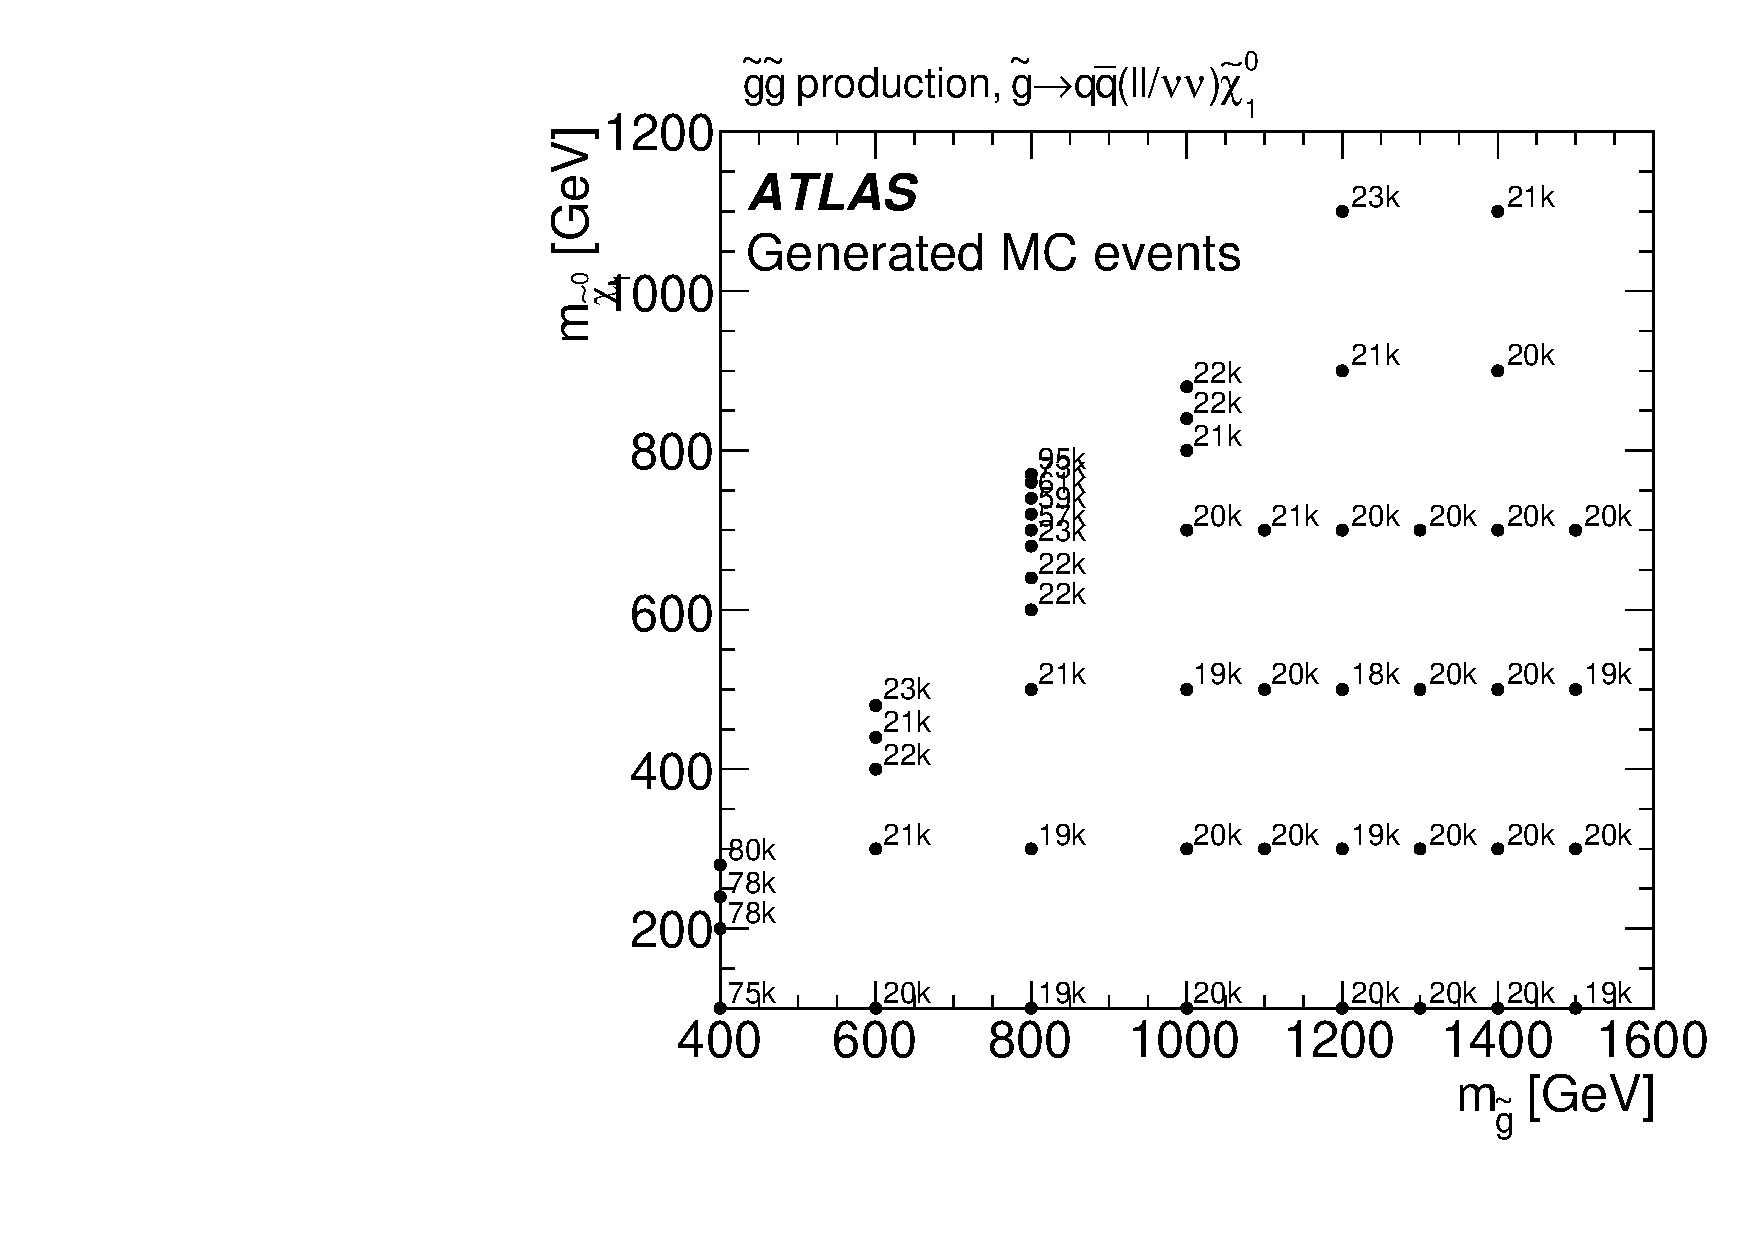
\includegraphics[width=\textwidth]{HEPDATA/mcstats_SR0b3j.pdf}
\caption{}\label{fig:hepdata_SR0b3j_mcstats}\end{subfigure}
\begin{subfigure}[t]{0.42\textwidth}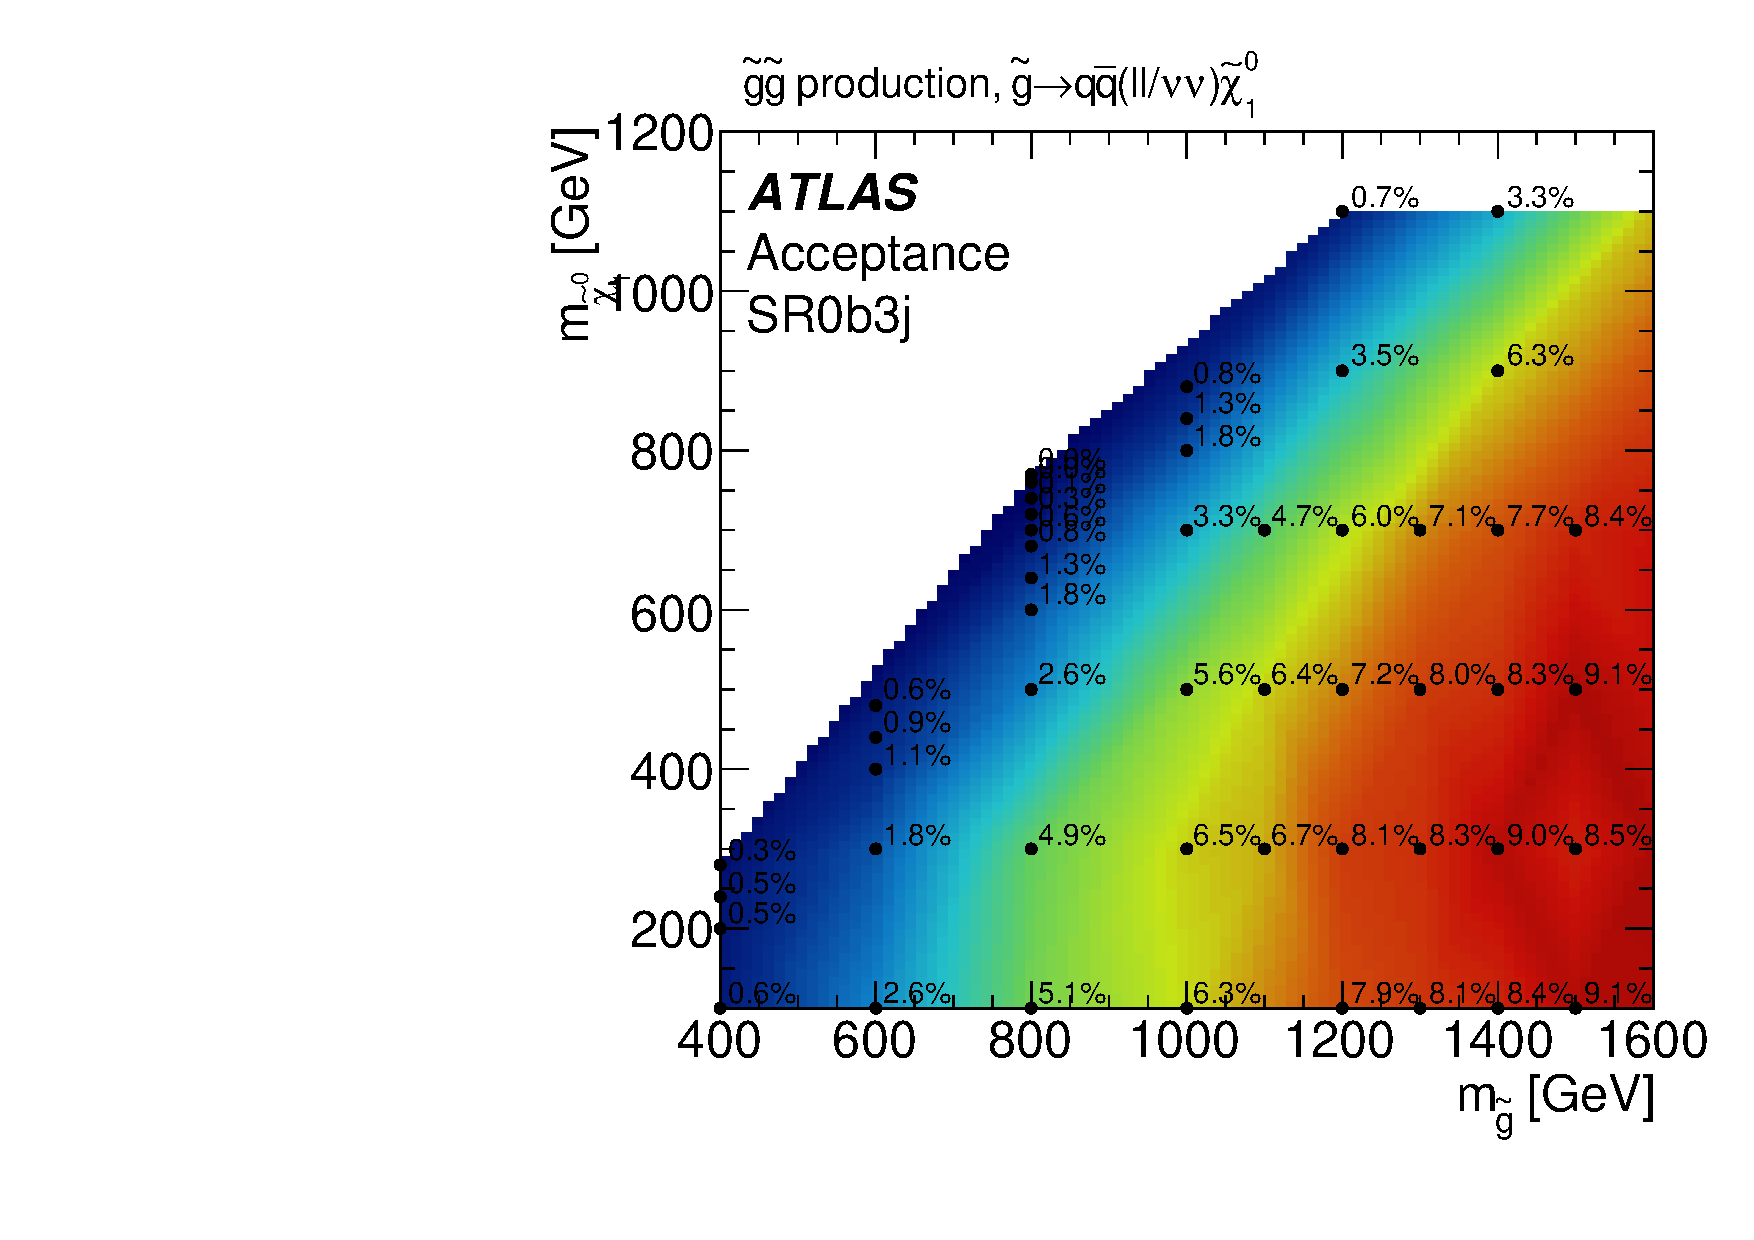
\includegraphics[width=\textwidth]{HEPDATA/acceptance_SR0b3j.pdf}
\caption{}\label{fig:hepdata_SR0b3j_acceptance}\end{subfigure}
\begin{subfigure}[t]{0.42\textwidth}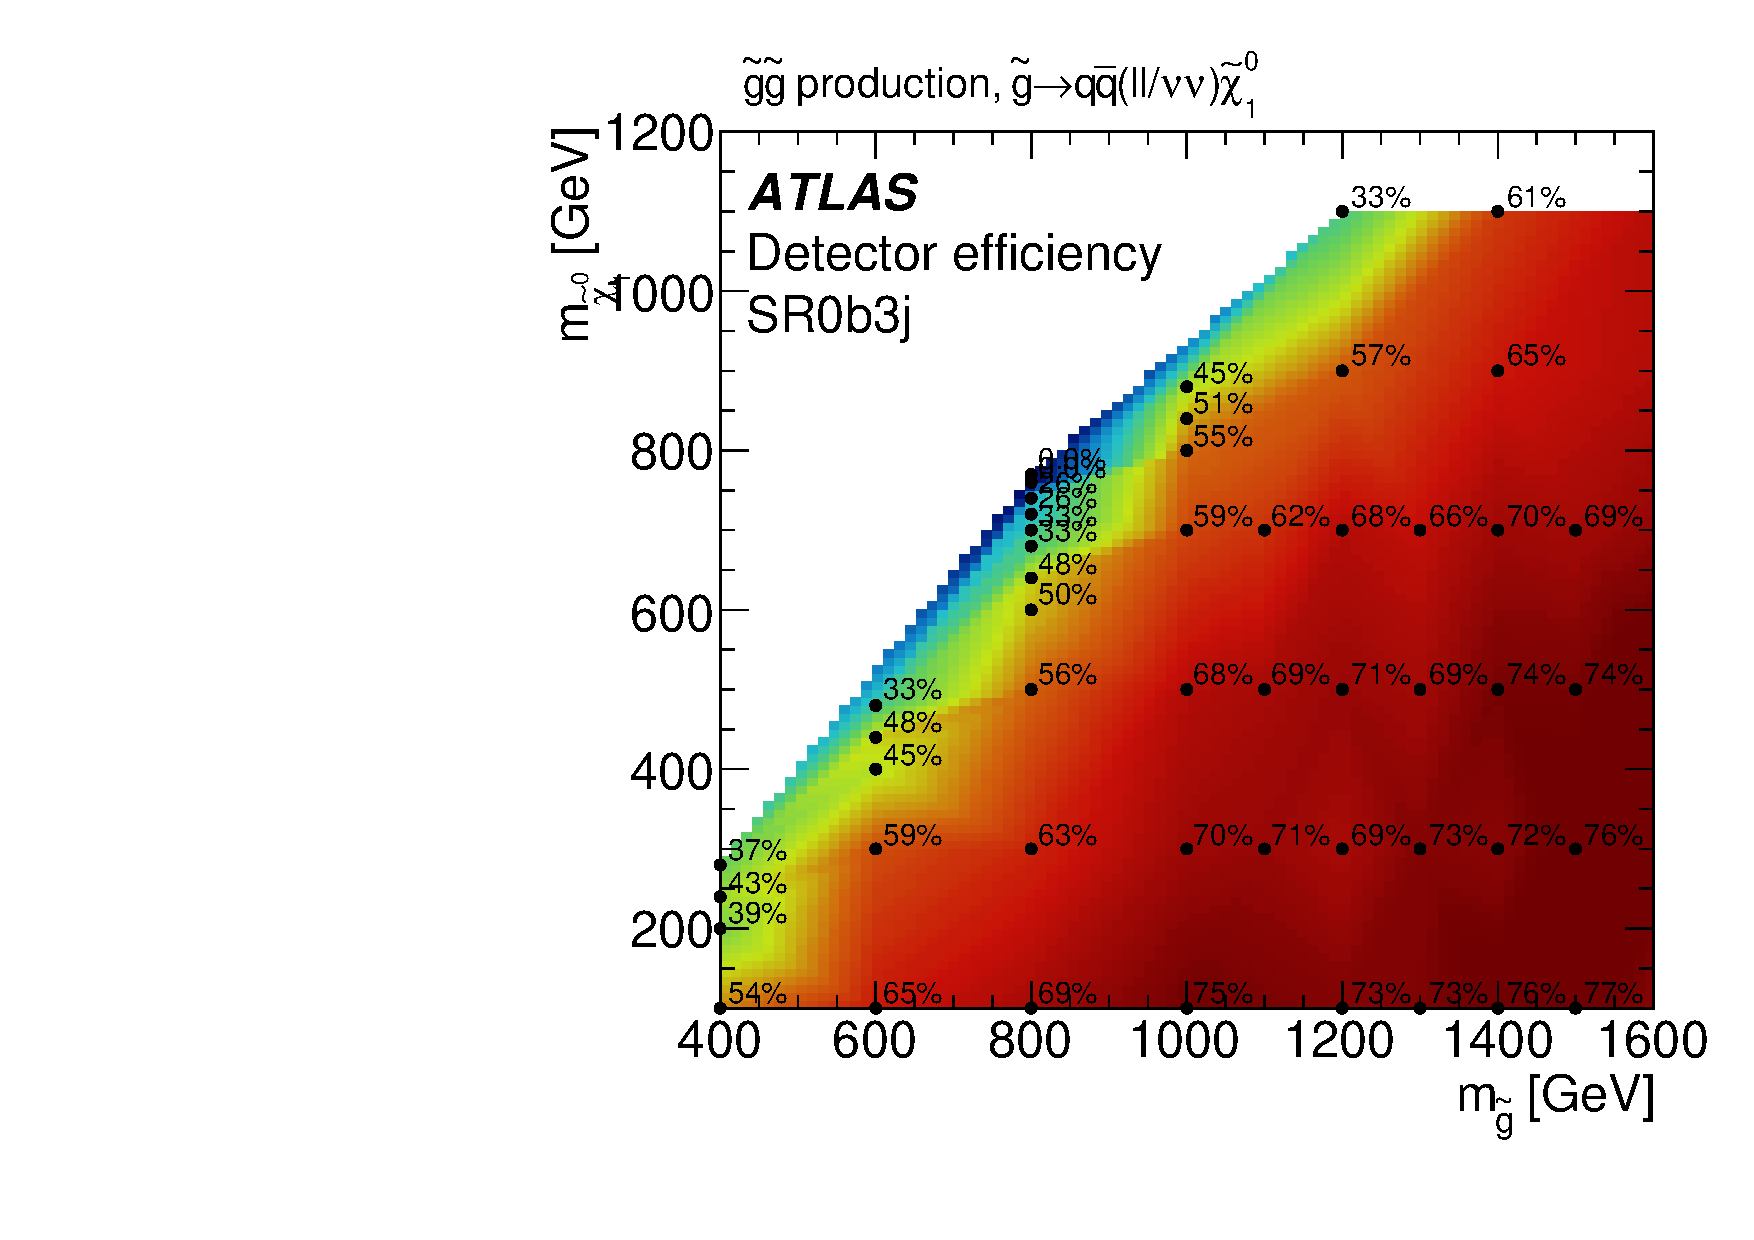
\includegraphics[width=\textwidth]{HEPDATA/efficiency_SR0b3j.pdf}
\caption{}\label{fig:hepdata_SR0b3j_efficiency}\end{subfigure}
\begin{subfigure}[t]{0.42\textwidth}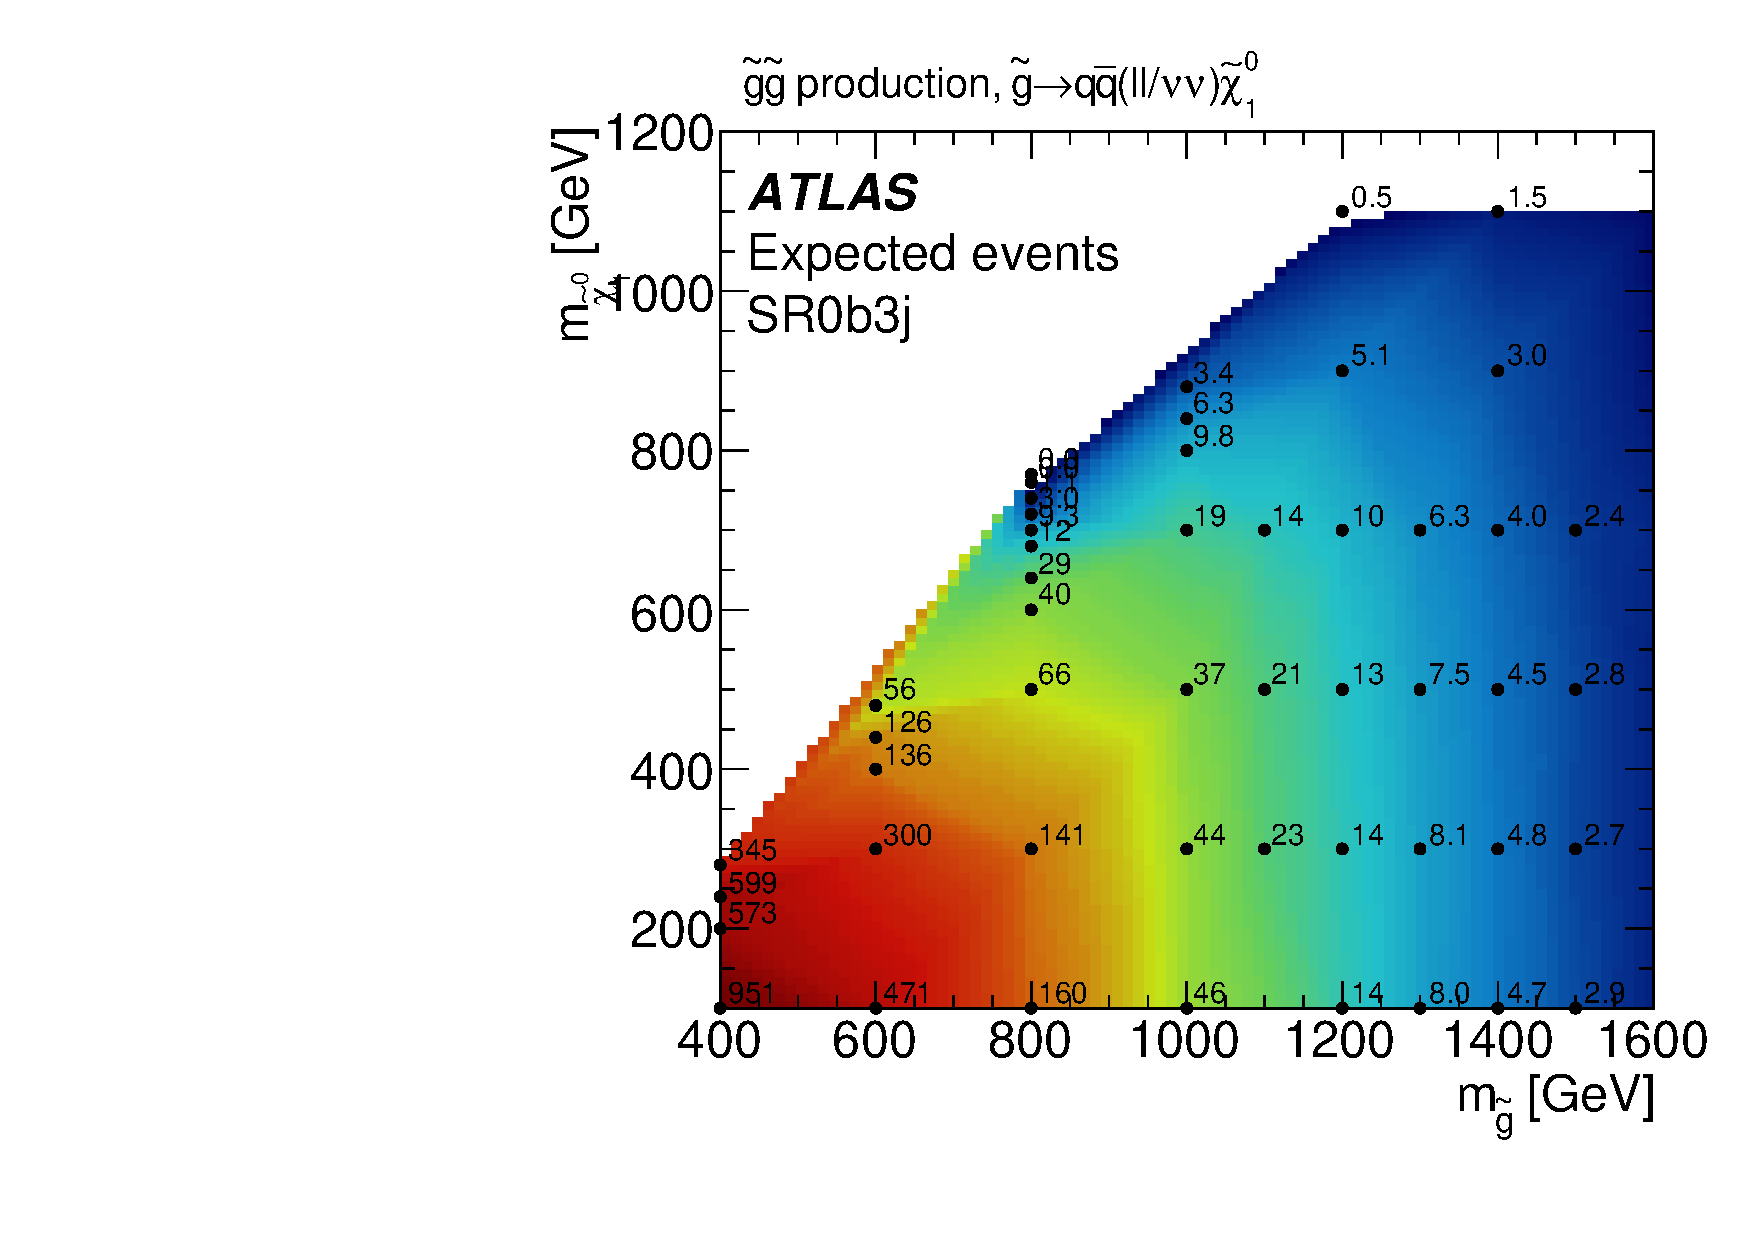
\includegraphics[width=\textwidth]{HEPDATA/yield_SR0b3j.pdf}
\caption{}\label{fig:hepdata_SR0b3j_yield}\end{subfigure}
\begin{subfigure}[t]{0.42\textwidth}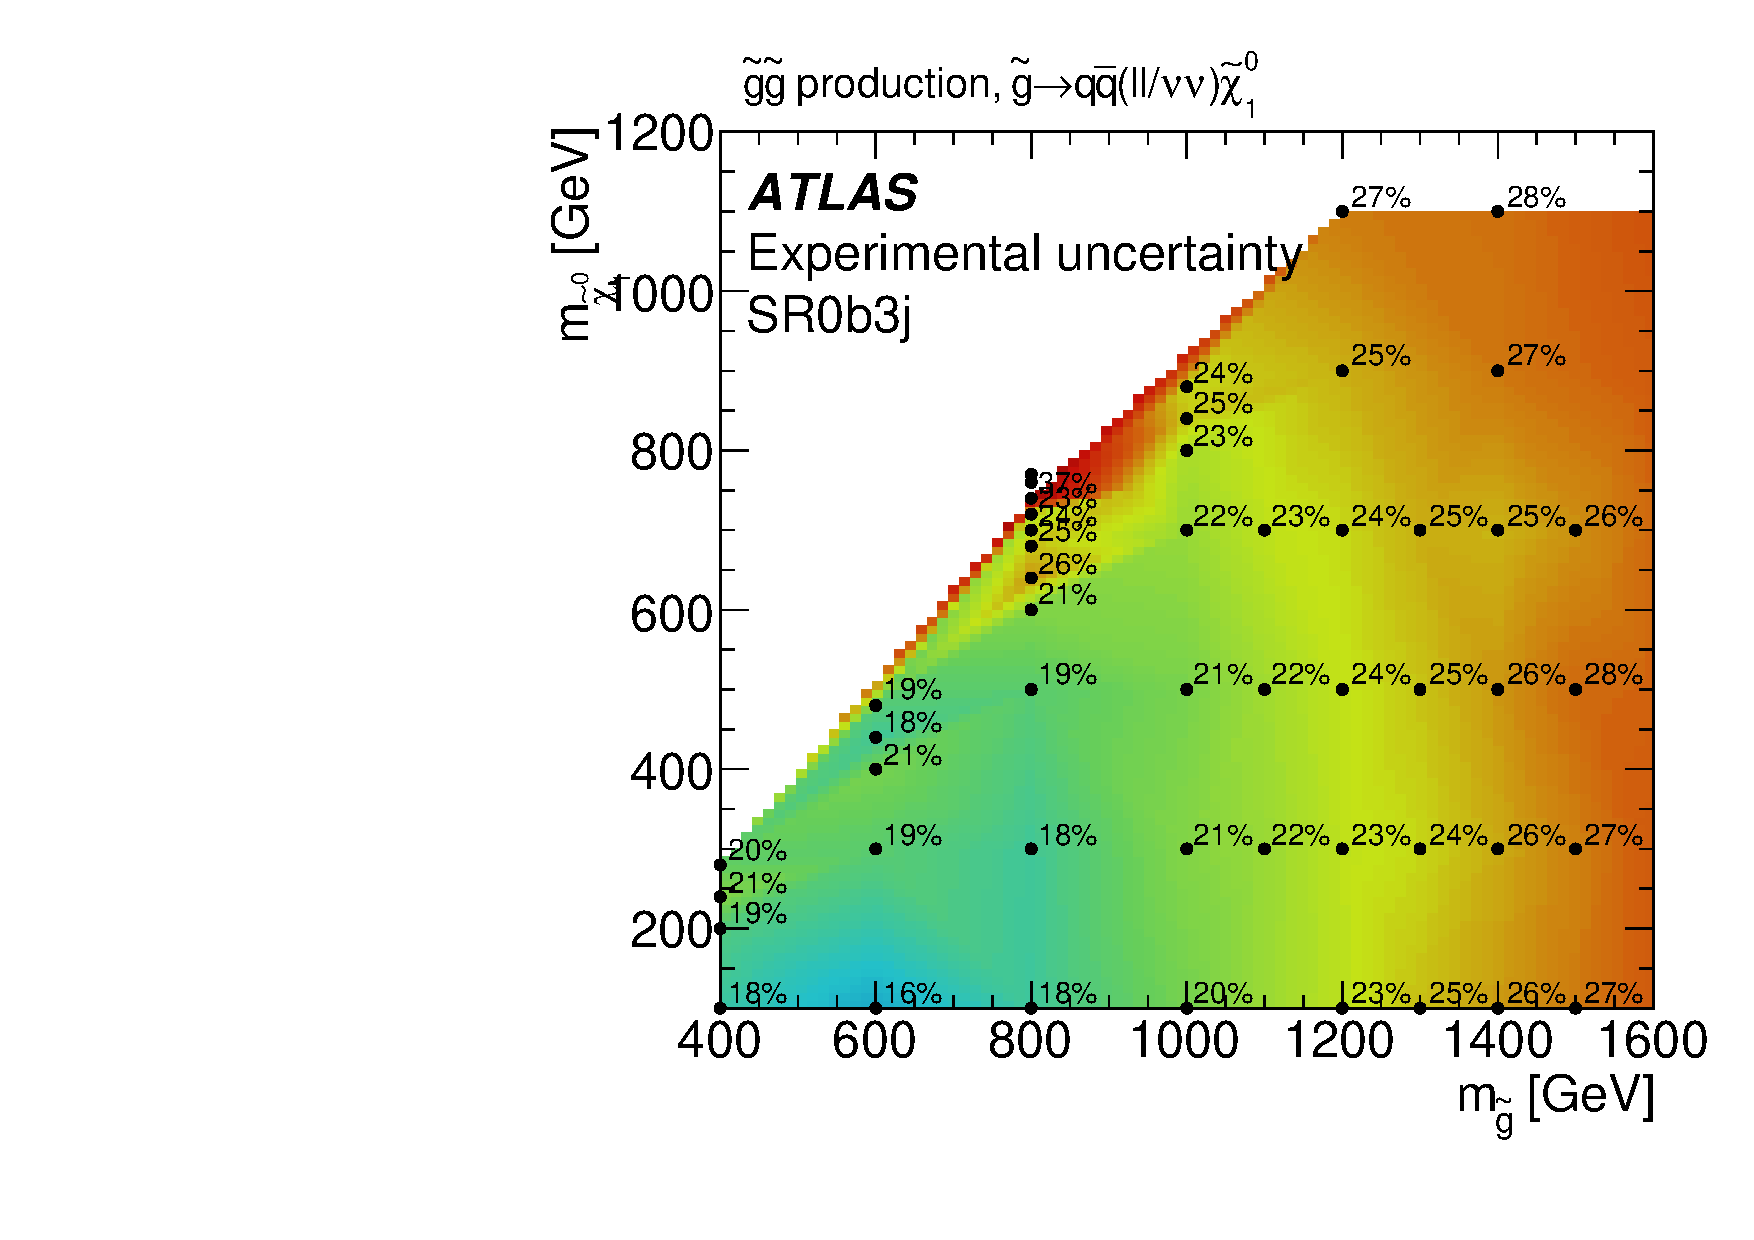
\includegraphics[width=\textwidth]{HEPDATA/mcsyst_SR0b3j.pdf}
\caption{}\label{fig:hepdata_SR0b3j_mcsyst}\end{subfigure}
\caption{SUSY scenario with $\gluino\gluino$ production and $\gluino\to q\bar q\ell\ell\ninoone$ decay: 
(a) production cross-section, (b) number of generated MC events, 
(c) signal acceptance and (d) reconstruction efficiency in the signal region SR0b3j, 
(e) corresponding expected signal yield and (f) associated uncertainty due to experimental sources. 
The benchmark scenarios used to set exclusion limits are materialized by black dot markers. 
Acceptance and efficiency are defined as in appendix~A of~\cite{Stop2L}.}
\label{fig:HepData_SR0b3j}
\end{figure}

\begin{figure}[p]
\centering
\begin{subfigure}[t]{0.42\textwidth}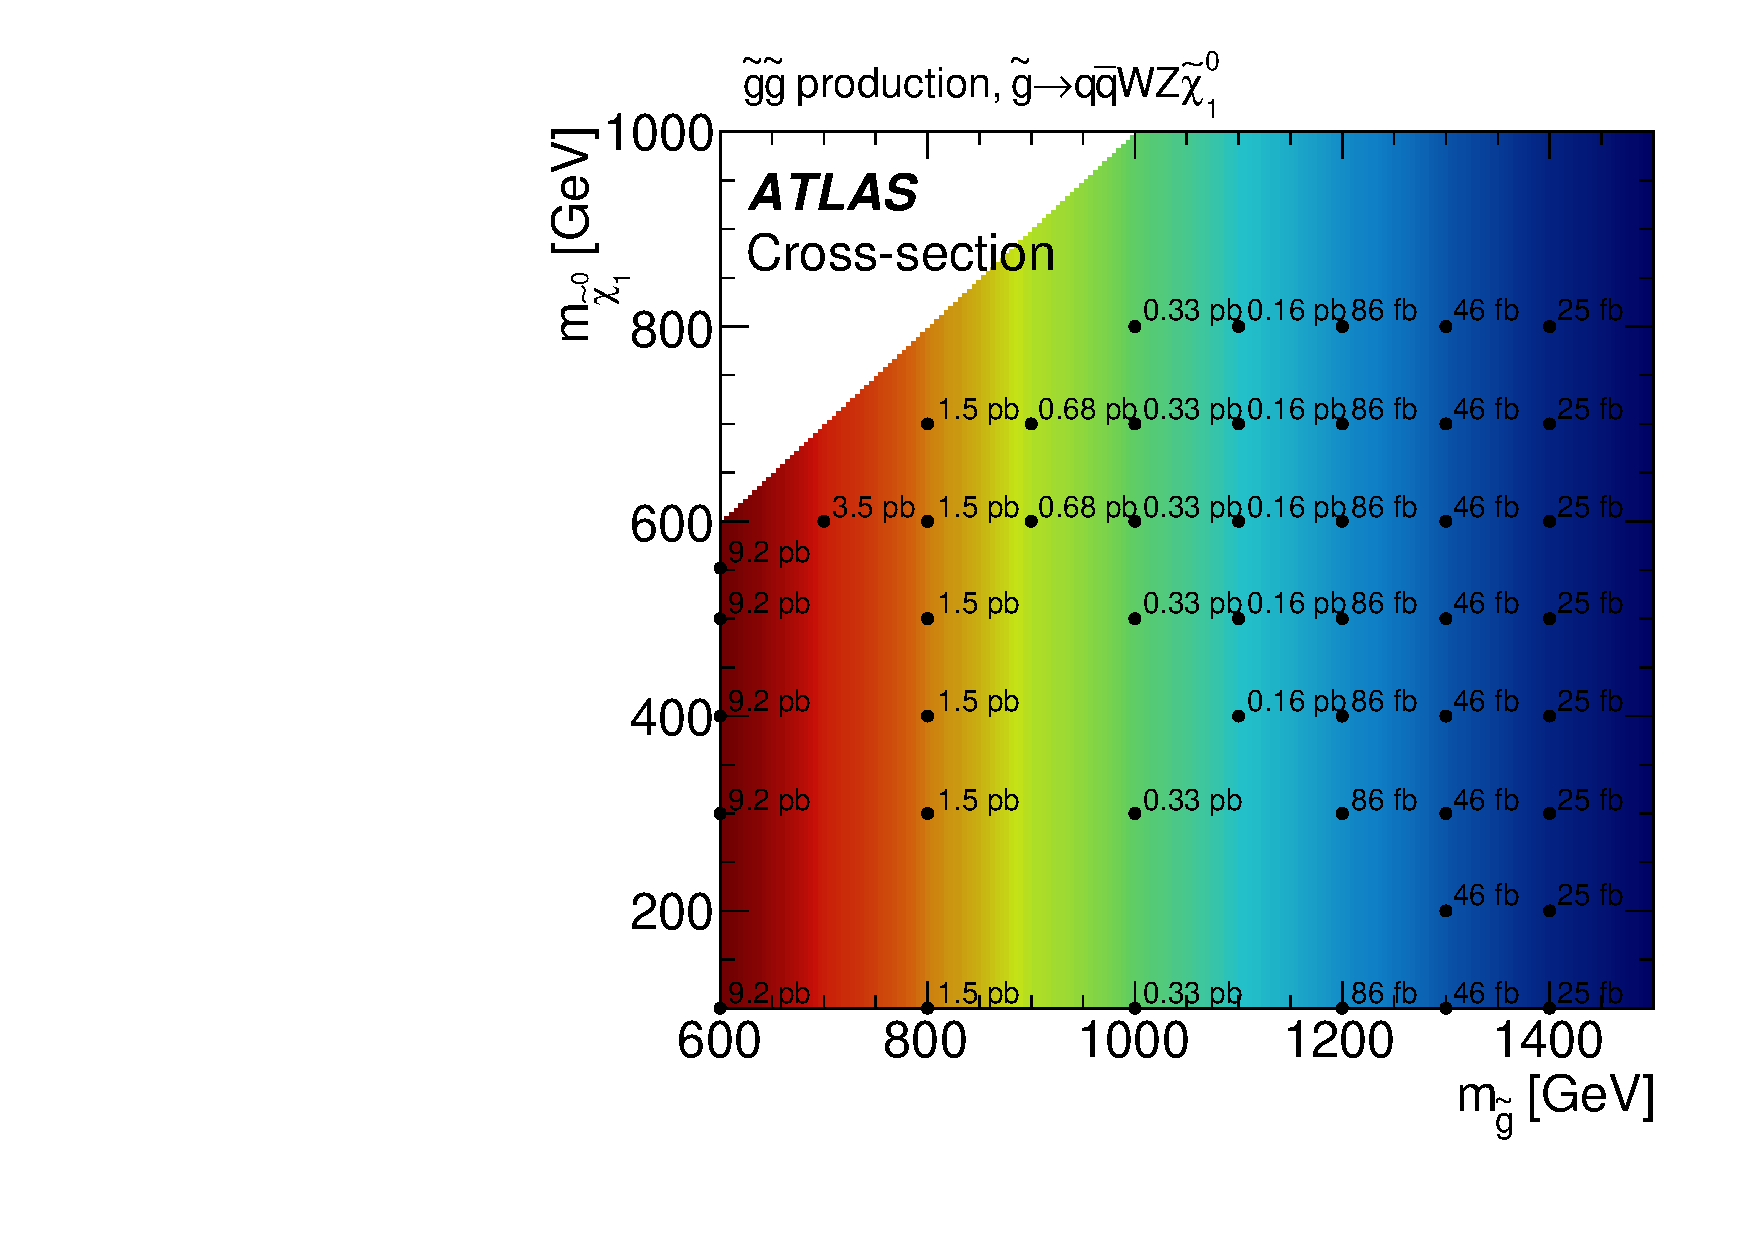
\includegraphics[width=\textwidth]{HEPDATA/xsection_SR0b5j.pdf}
\caption{}\label{fig:hepdata_SR0b5j_xsection}\end{subfigure}
\begin{subfigure}[t]{0.42\textwidth}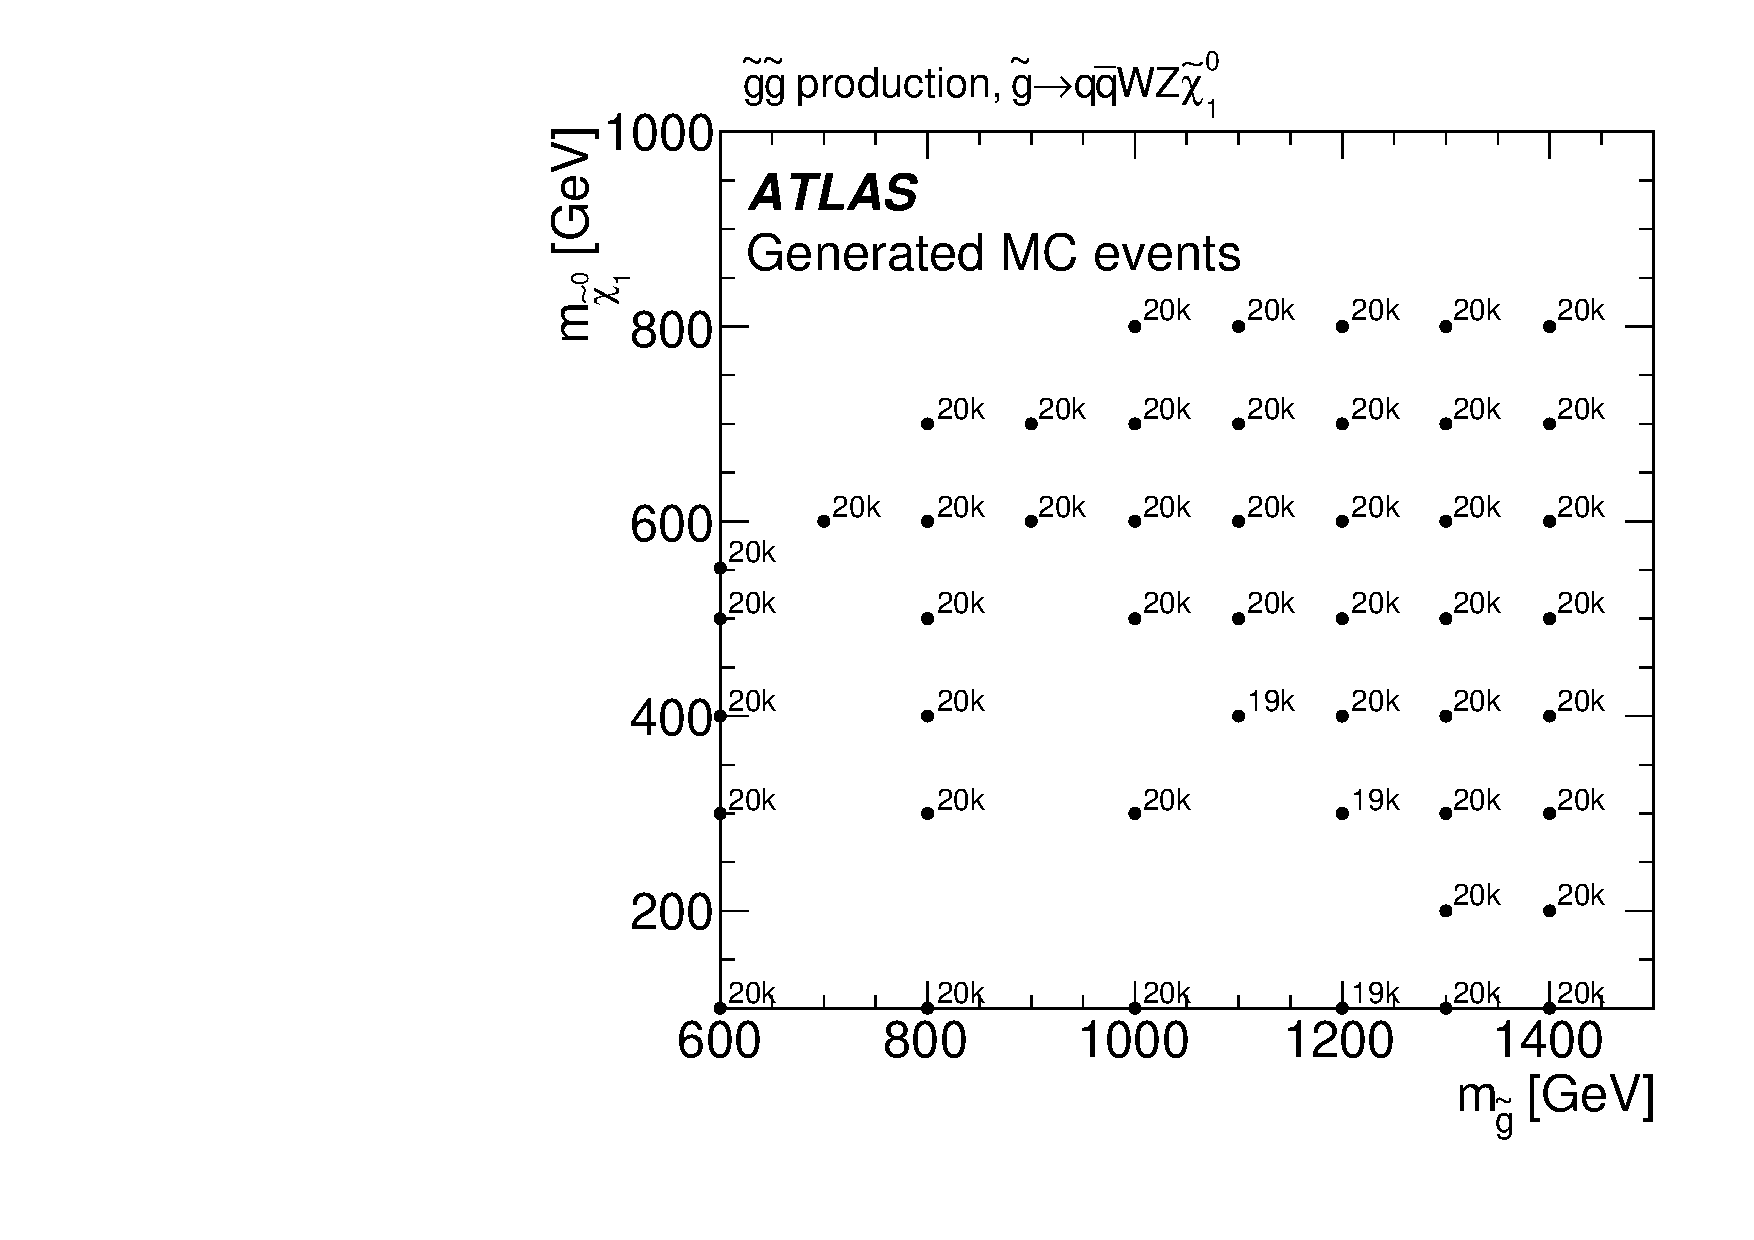
\includegraphics[width=\textwidth]{HEPDATA/mcstats_SR0b5j.pdf}
\caption{}\label{fig:hepdata_SR0b5j_mcstats}\end{subfigure}
\begin{subfigure}[t]{0.42\textwidth}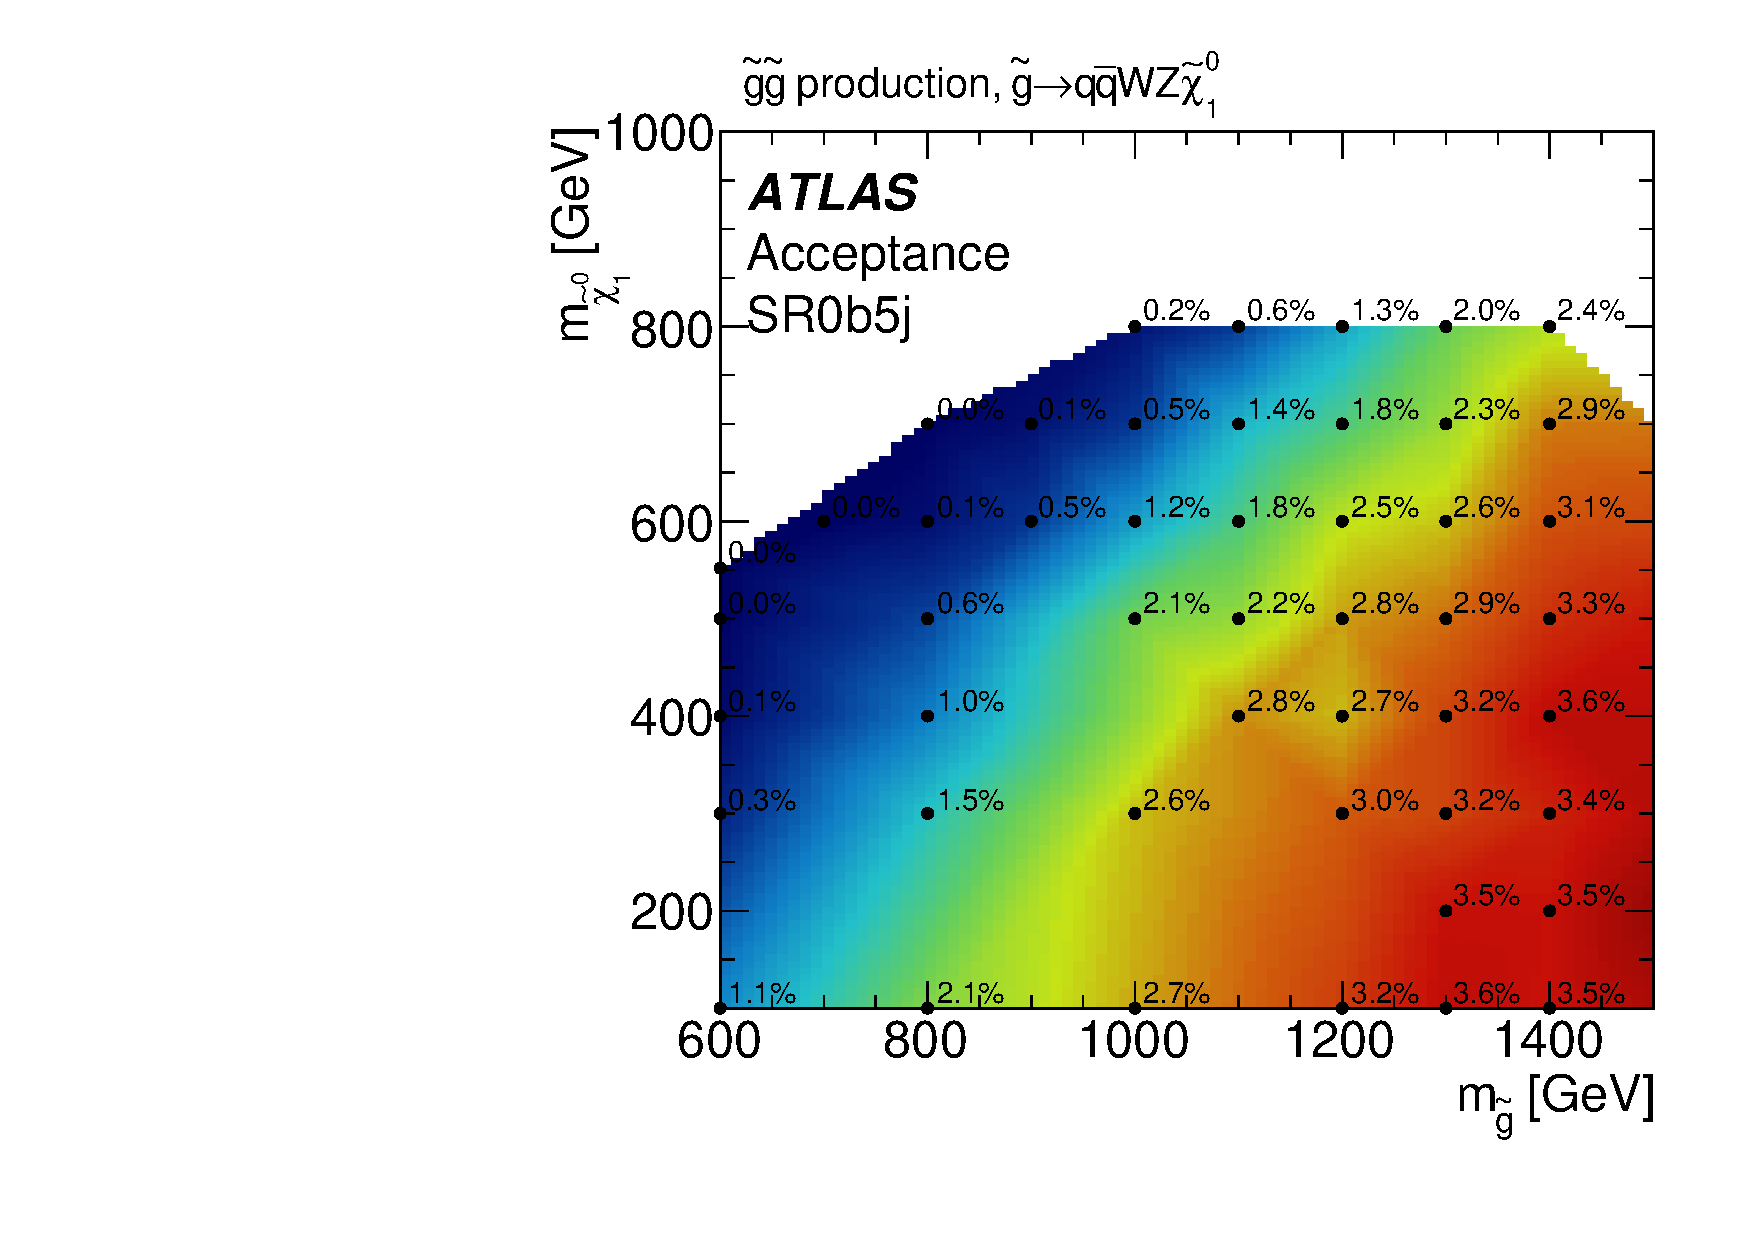
\includegraphics[width=\textwidth]{HEPDATA/acceptance_SR0b5j.pdf}
\caption{}\label{fig:hepdata_SR0b5j_acceptance}\end{subfigure}
\begin{subfigure}[t]{0.42\textwidth}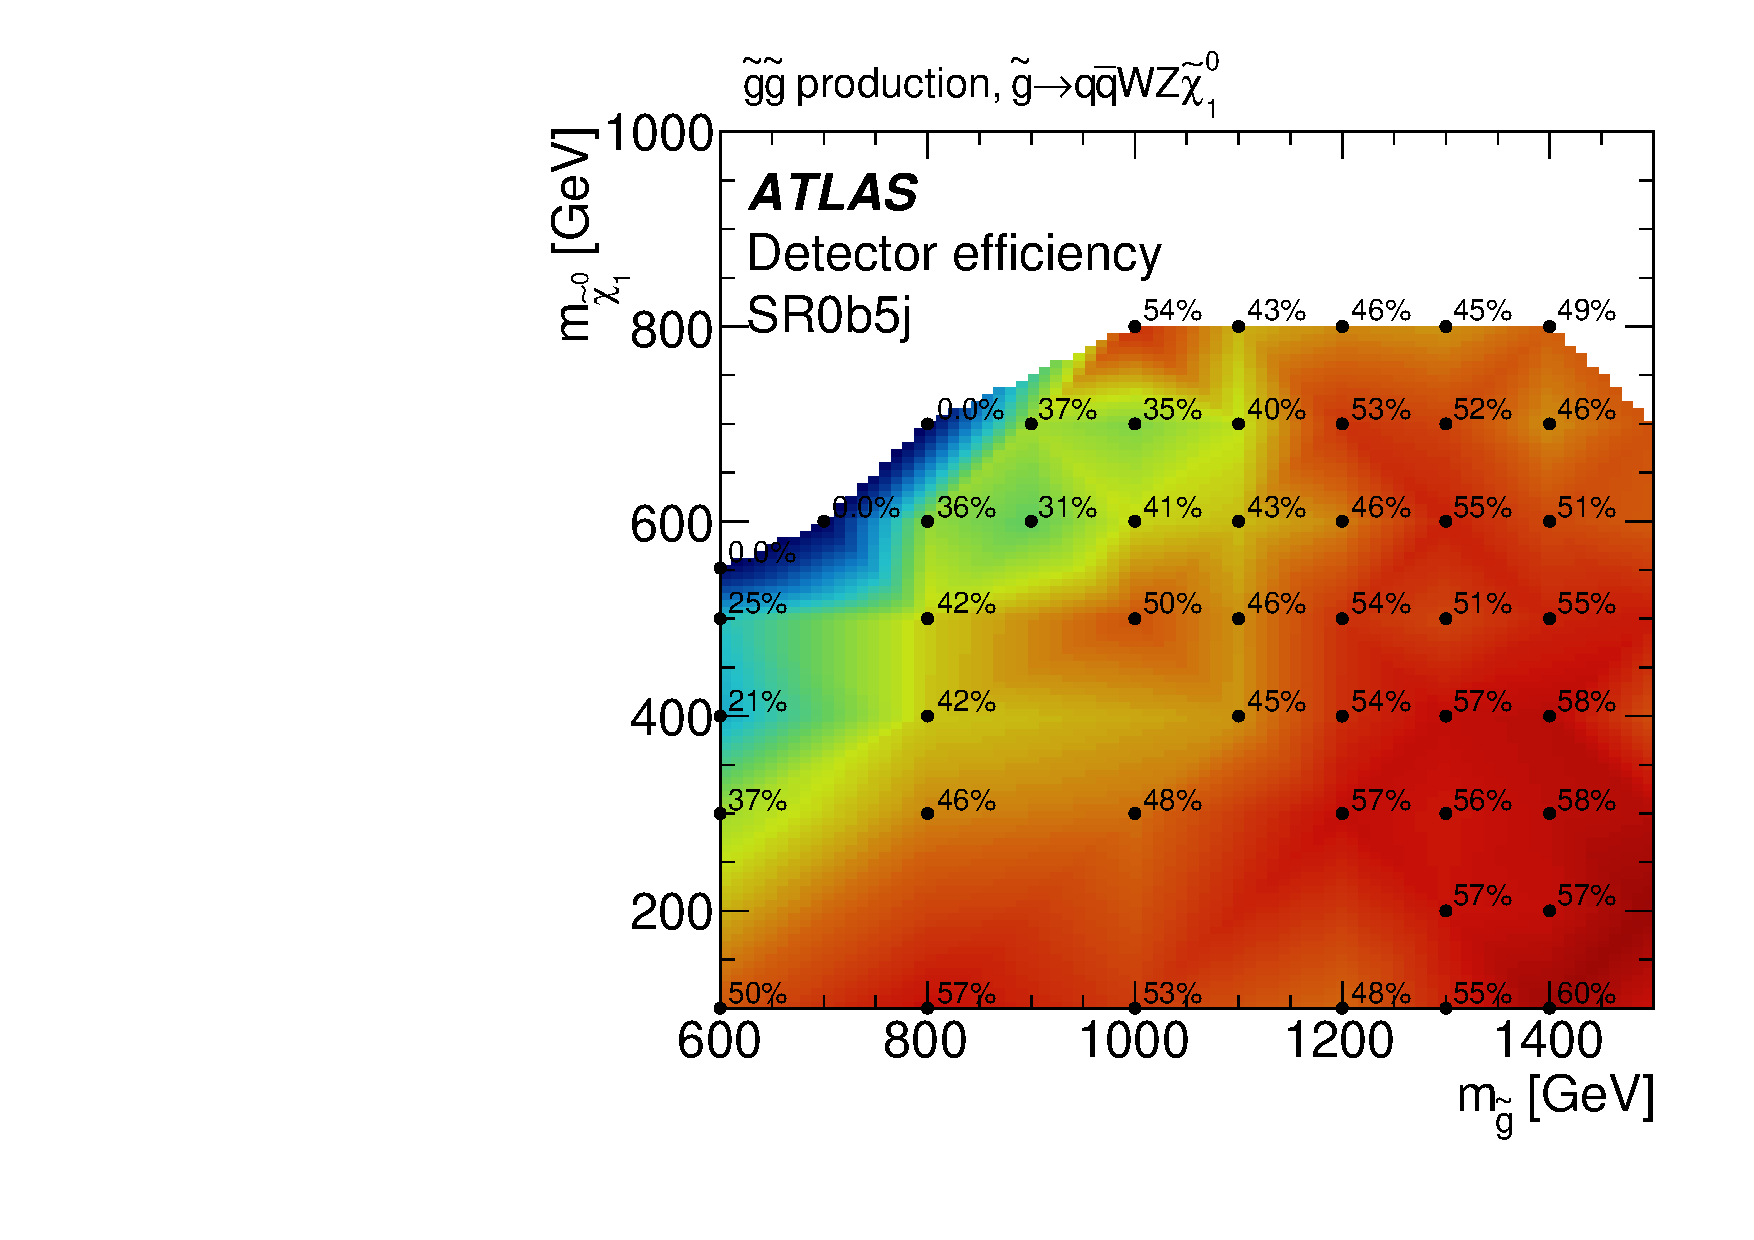
\includegraphics[width=\textwidth]{HEPDATA/efficiency_SR0b5j.pdf}
\caption{}\label{fig:hepdata_SR0b5j_efficiency}\end{subfigure}
\begin{subfigure}[t]{0.42\textwidth}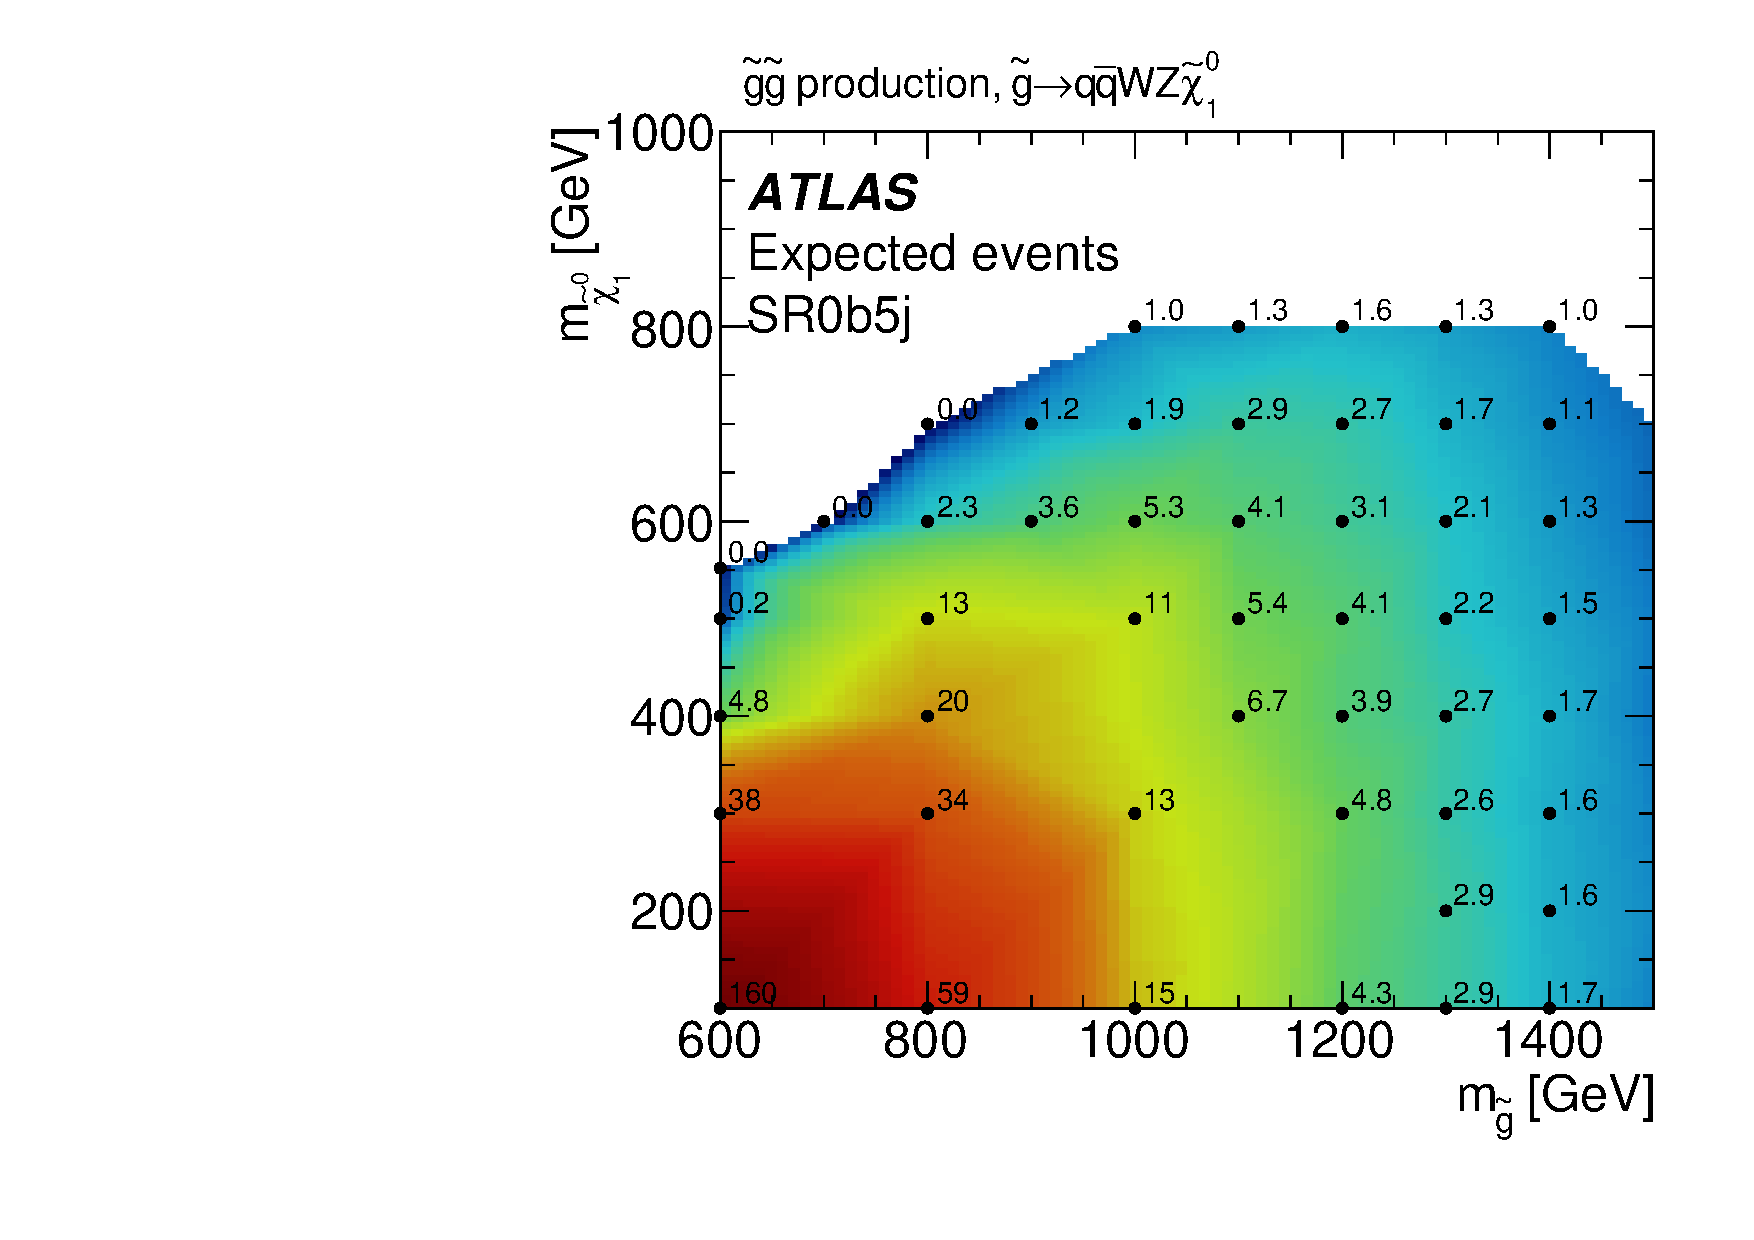
\includegraphics[width=\textwidth]{HEPDATA/yield_SR0b5j.pdf}
\caption{}\label{fig:hepdata_SR0b5j_yield}\end{subfigure}
\begin{subfigure}[t]{0.42\textwidth}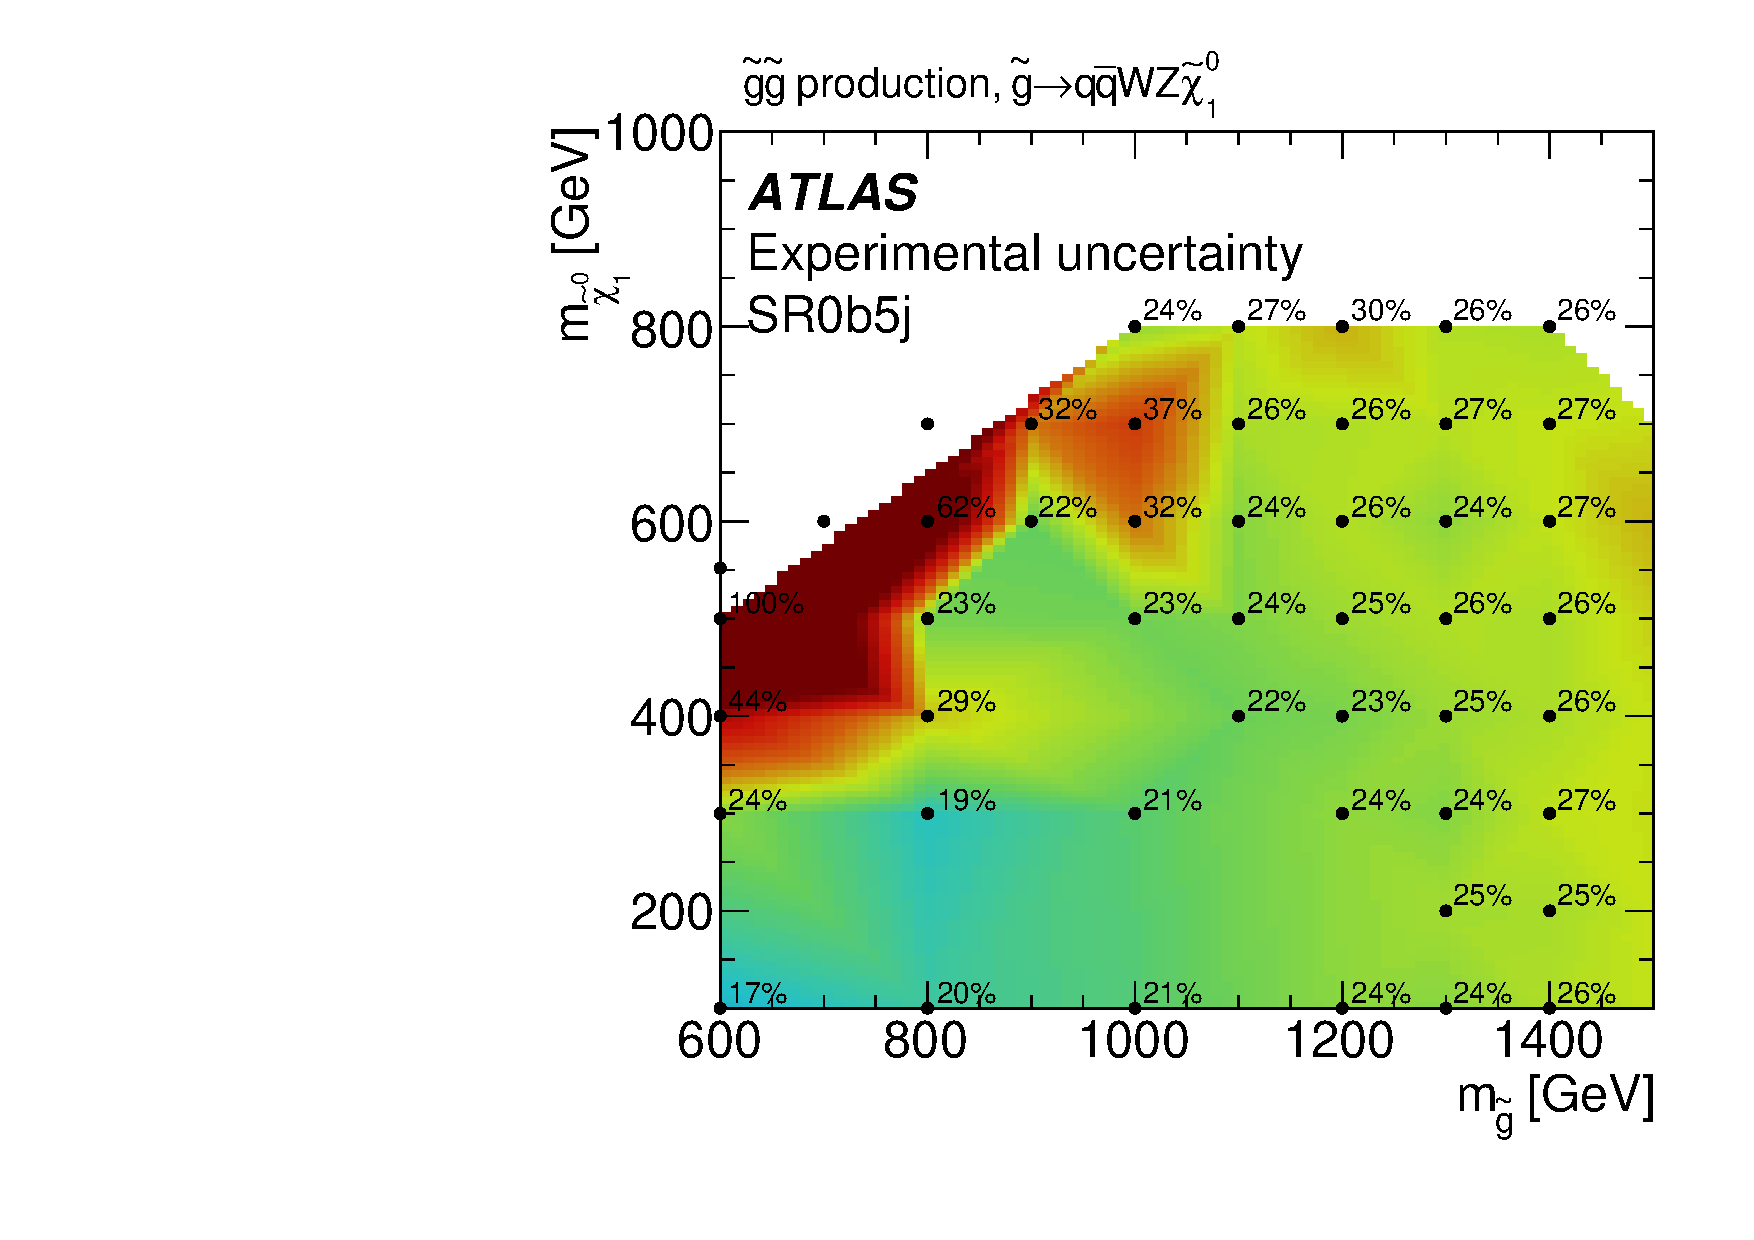
\includegraphics[width=\textwidth]{HEPDATA/mcsyst_SR0b5j.pdf}
\caption{}\label{fig:hepdata_SR0b5j_mcsyst}\end{subfigure}
\caption{SUSY scenario with $\gluino\gluino$ production and $\gluino\to q\bar qWZ\ninoone$ decay: 
(a) production cross-section, (b) number of generated MC events, 
(c) signal acceptance and (d) reconstruction efficiency in the signal region SR0b5j, 
(e) corresponding expected signal yield and (f) associated uncertainty due to experimental sources. 
The benchmark scenarios used to set exclusion limits are materialized by black dot markers. 
Acceptance and efficiency are defined as in appendix~A of~\cite{Stop2L}.}
\label{fig:HepData_SR0b5j} 
\end{figure}

\begin{figure}[p]
\centering
\begin{subfigure}[t]{0.42\textwidth}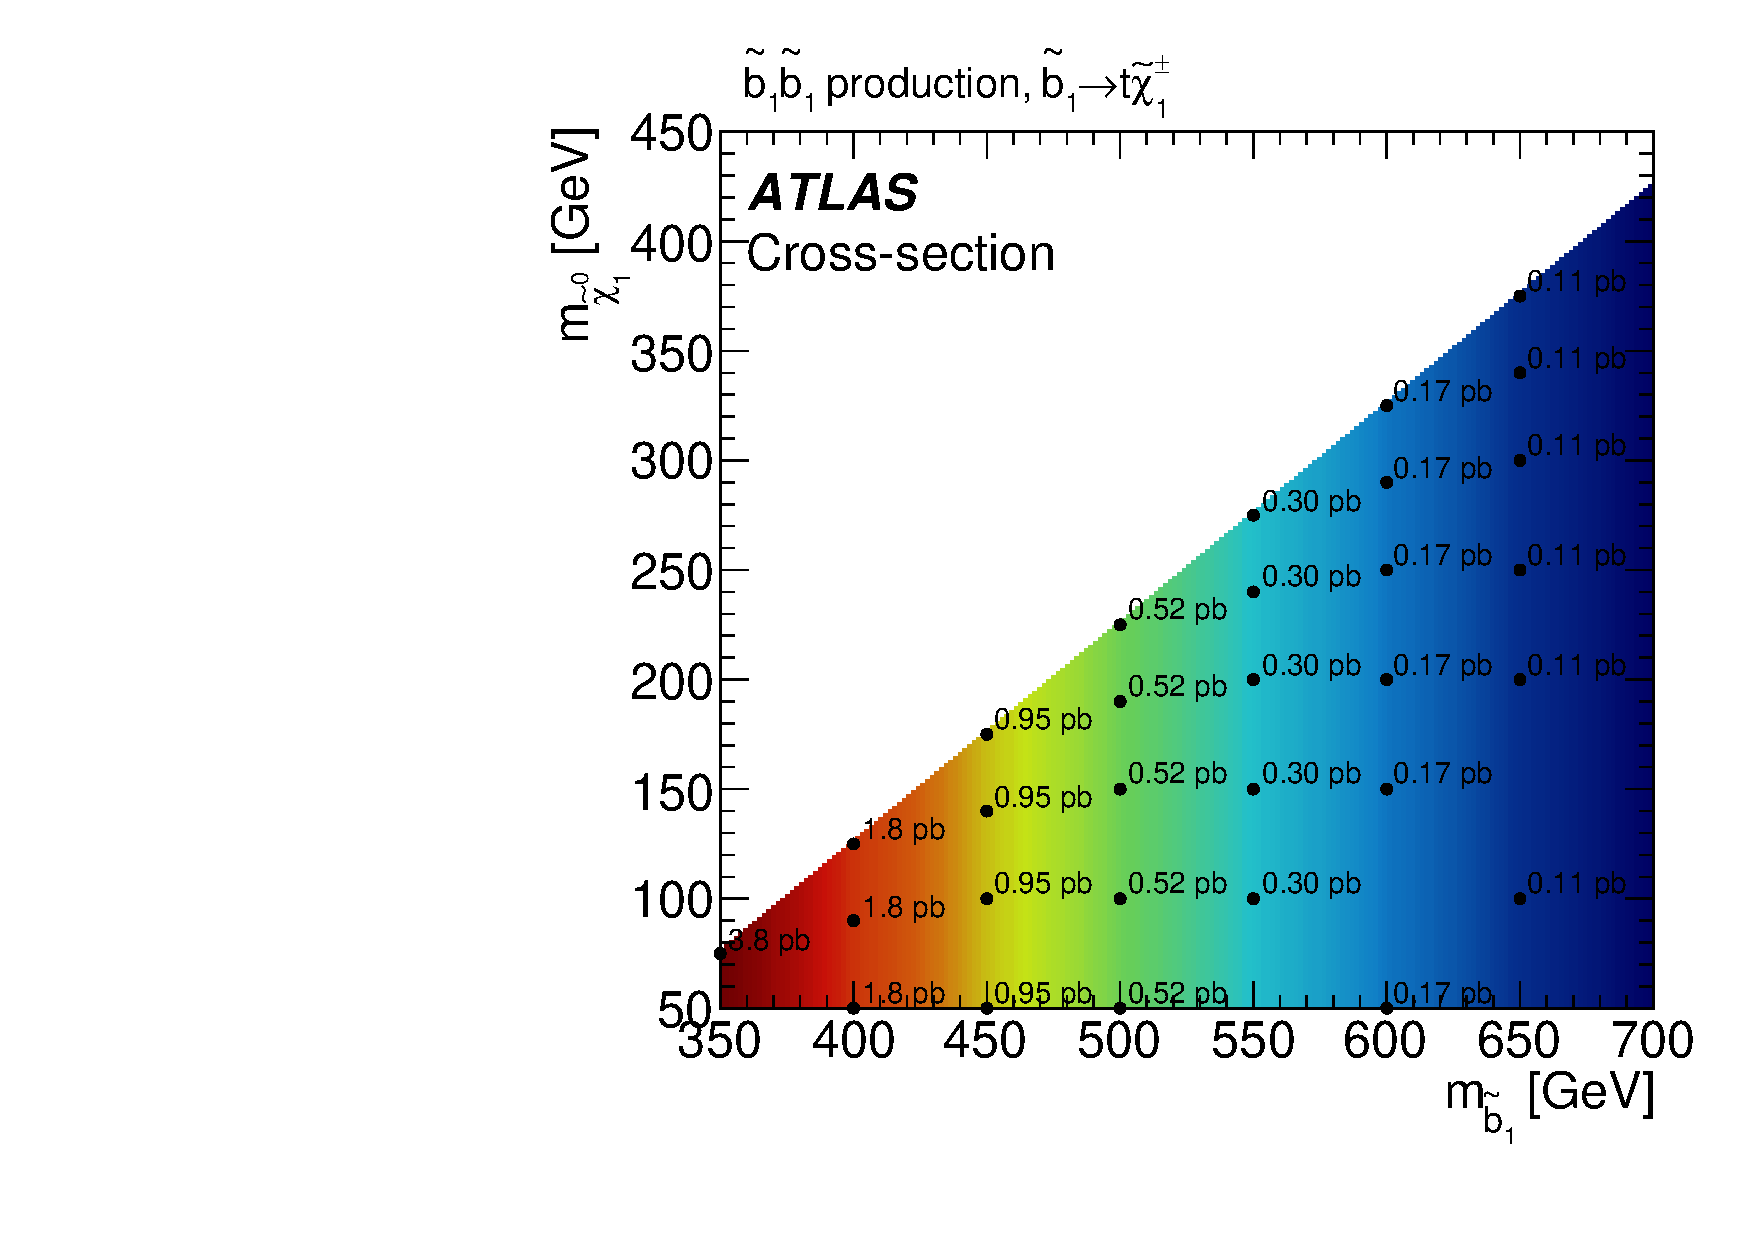
\includegraphics[width=\textwidth]{HEPDATA/xsection_SR1b.pdf}
\caption{}\label{fig:hepdata_SR1b_xsection}\end{subfigure}
\begin{subfigure}[t]{0.42\textwidth}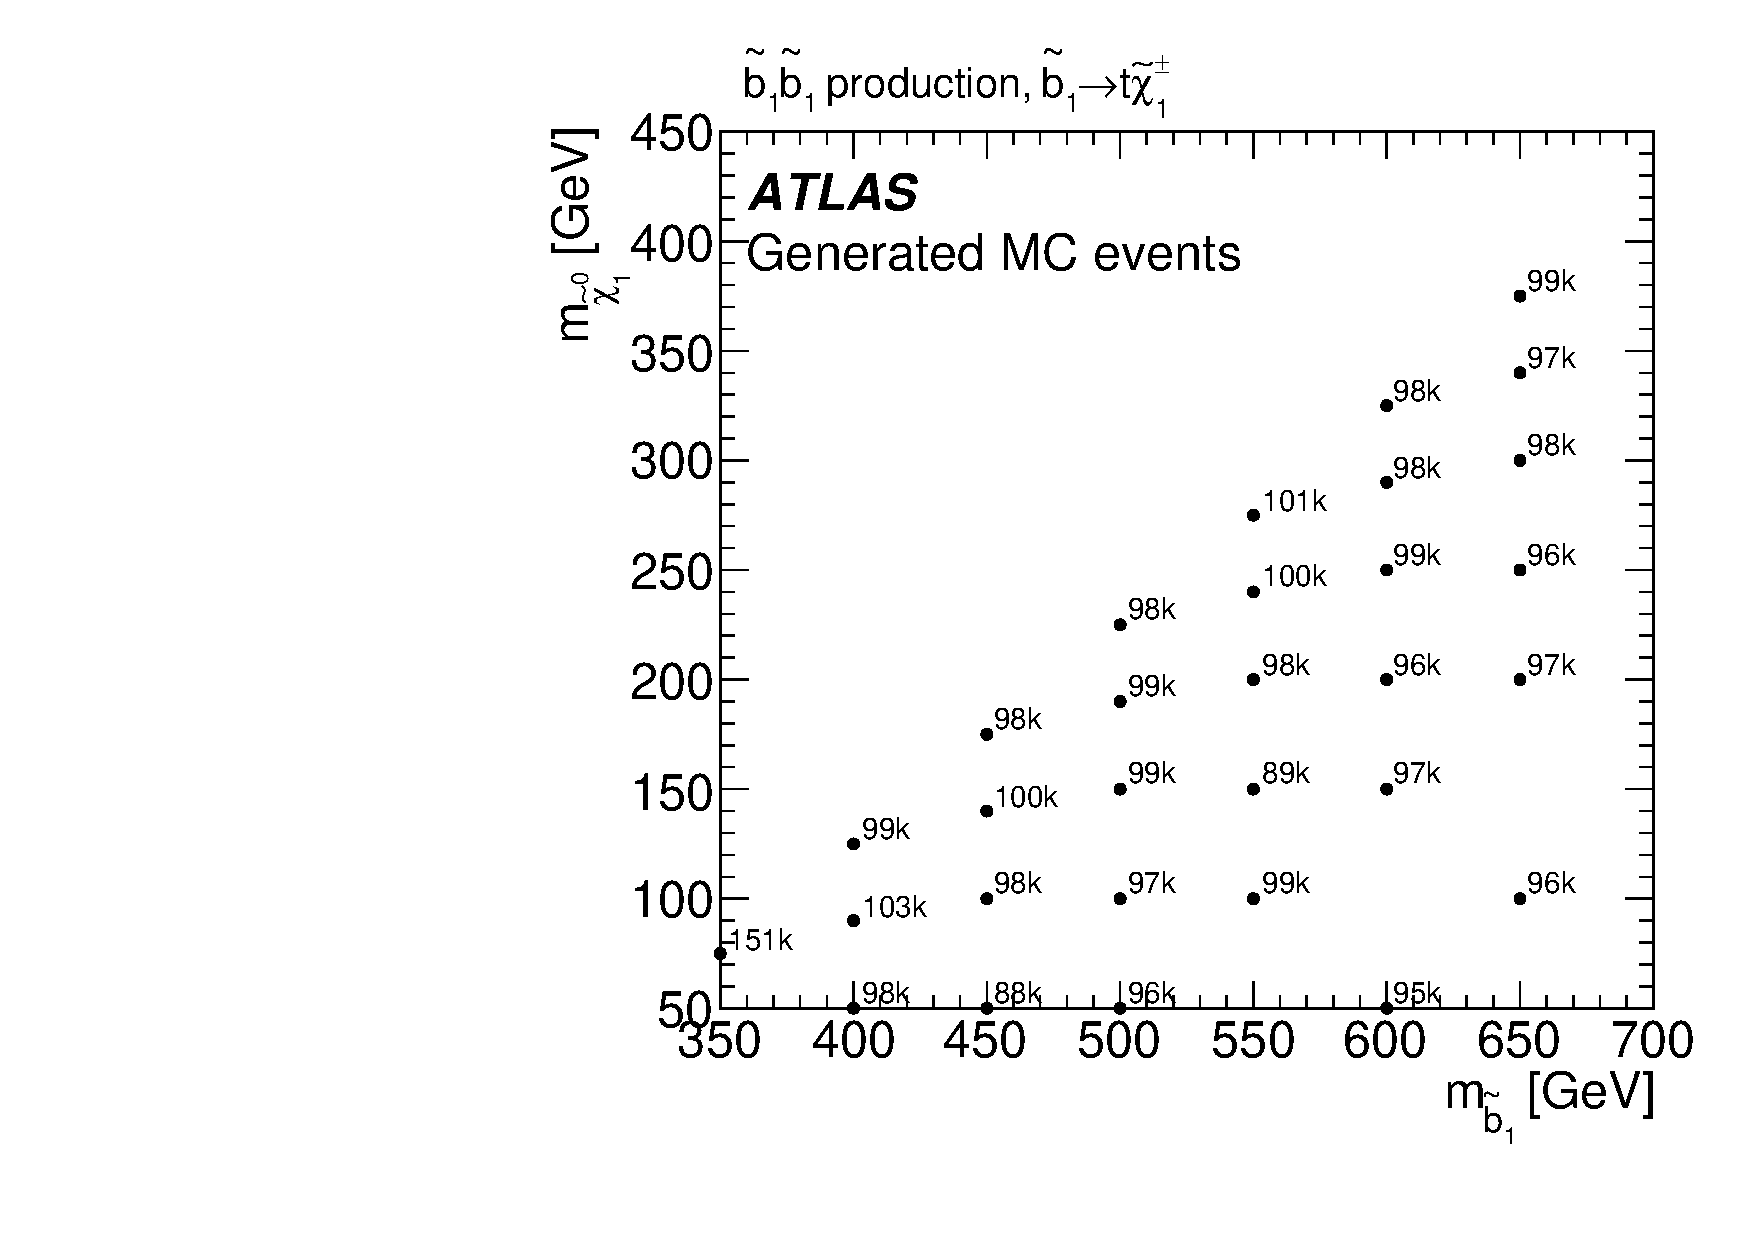
\includegraphics[width=\textwidth]{HEPDATA/mcstats_SR1b.pdf}
\caption{}\label{fig:hepdata_SR1b_mcstats}\end{subfigure}
\begin{subfigure}[t]{0.42\textwidth}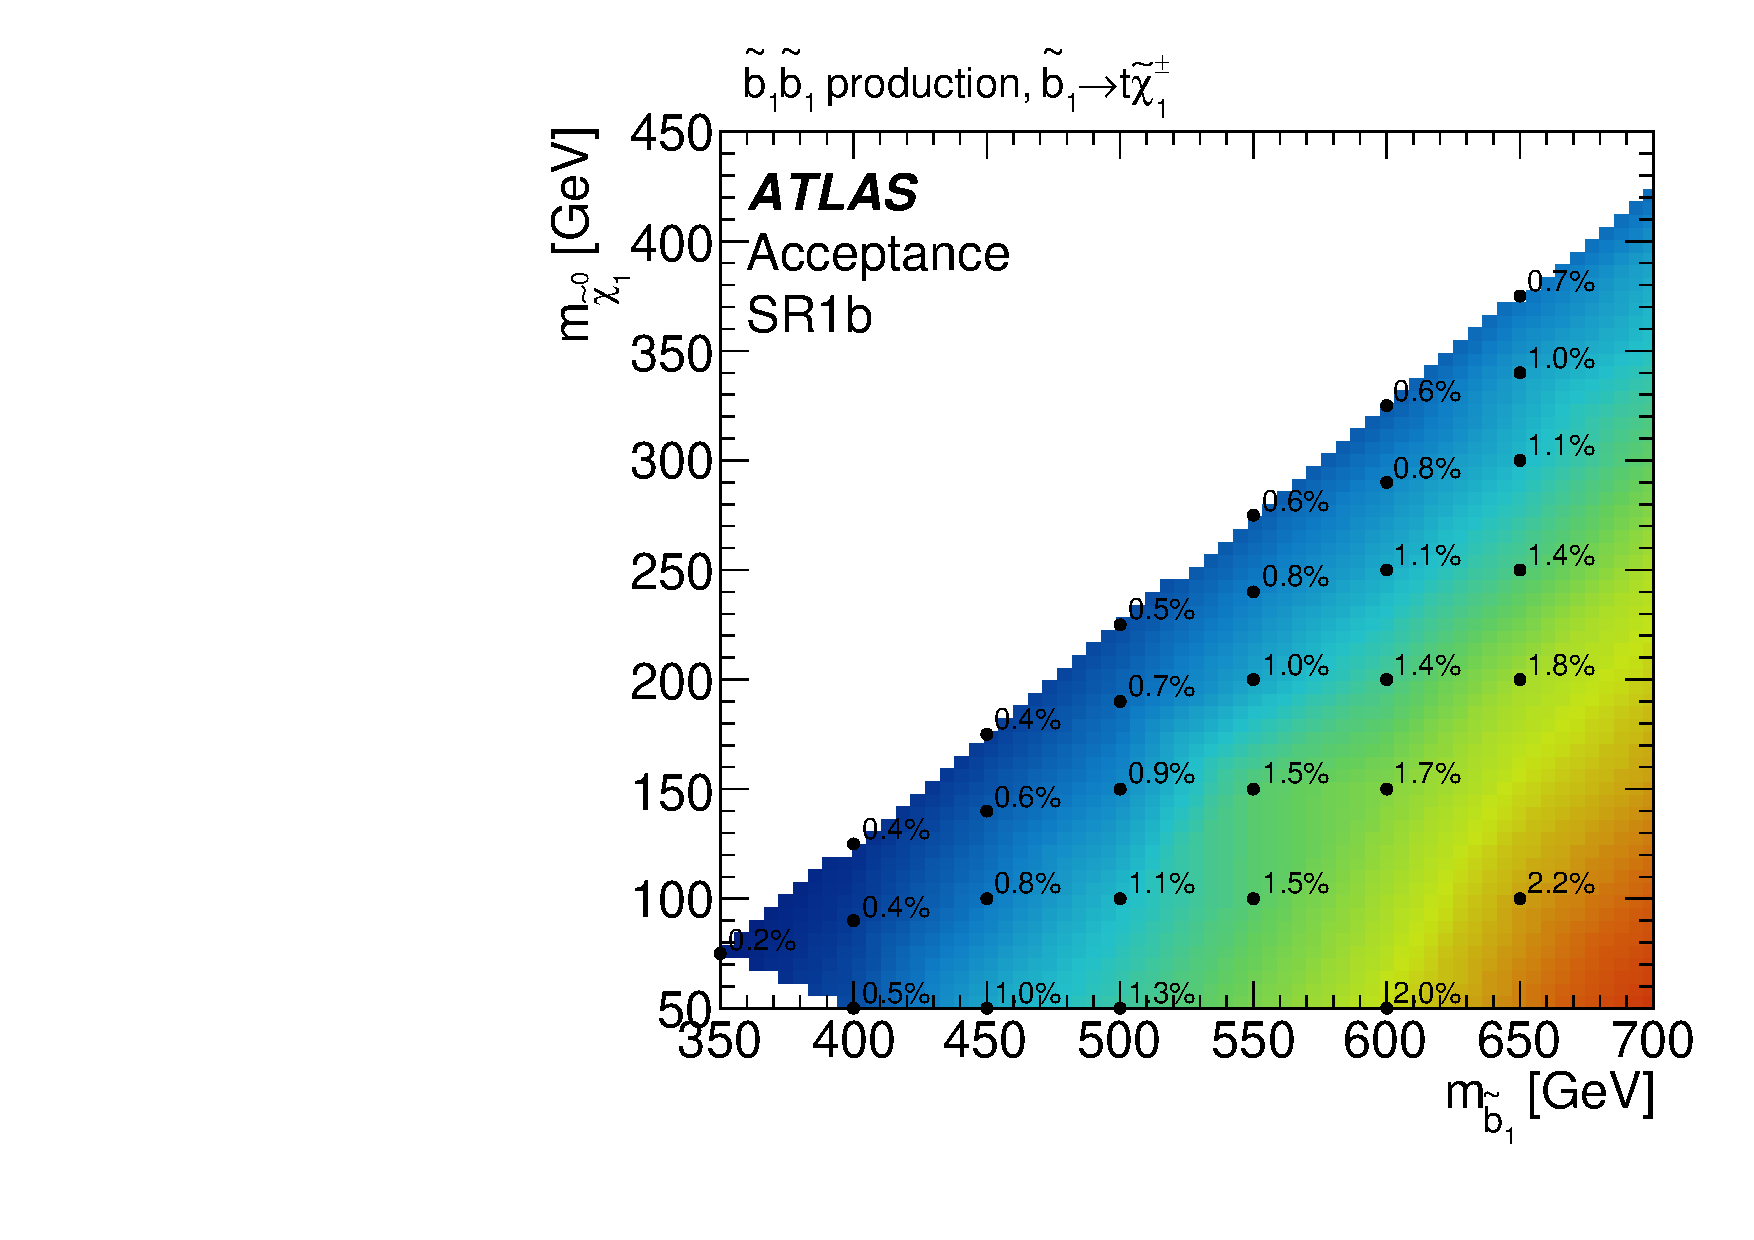
\includegraphics[width=\textwidth]{HEPDATA/acceptance_SR1b.pdf}
\caption{}\label{fig:hepdata_SR1b_acceptance}\end{subfigure}
\begin{subfigure}[t]{0.42\textwidth}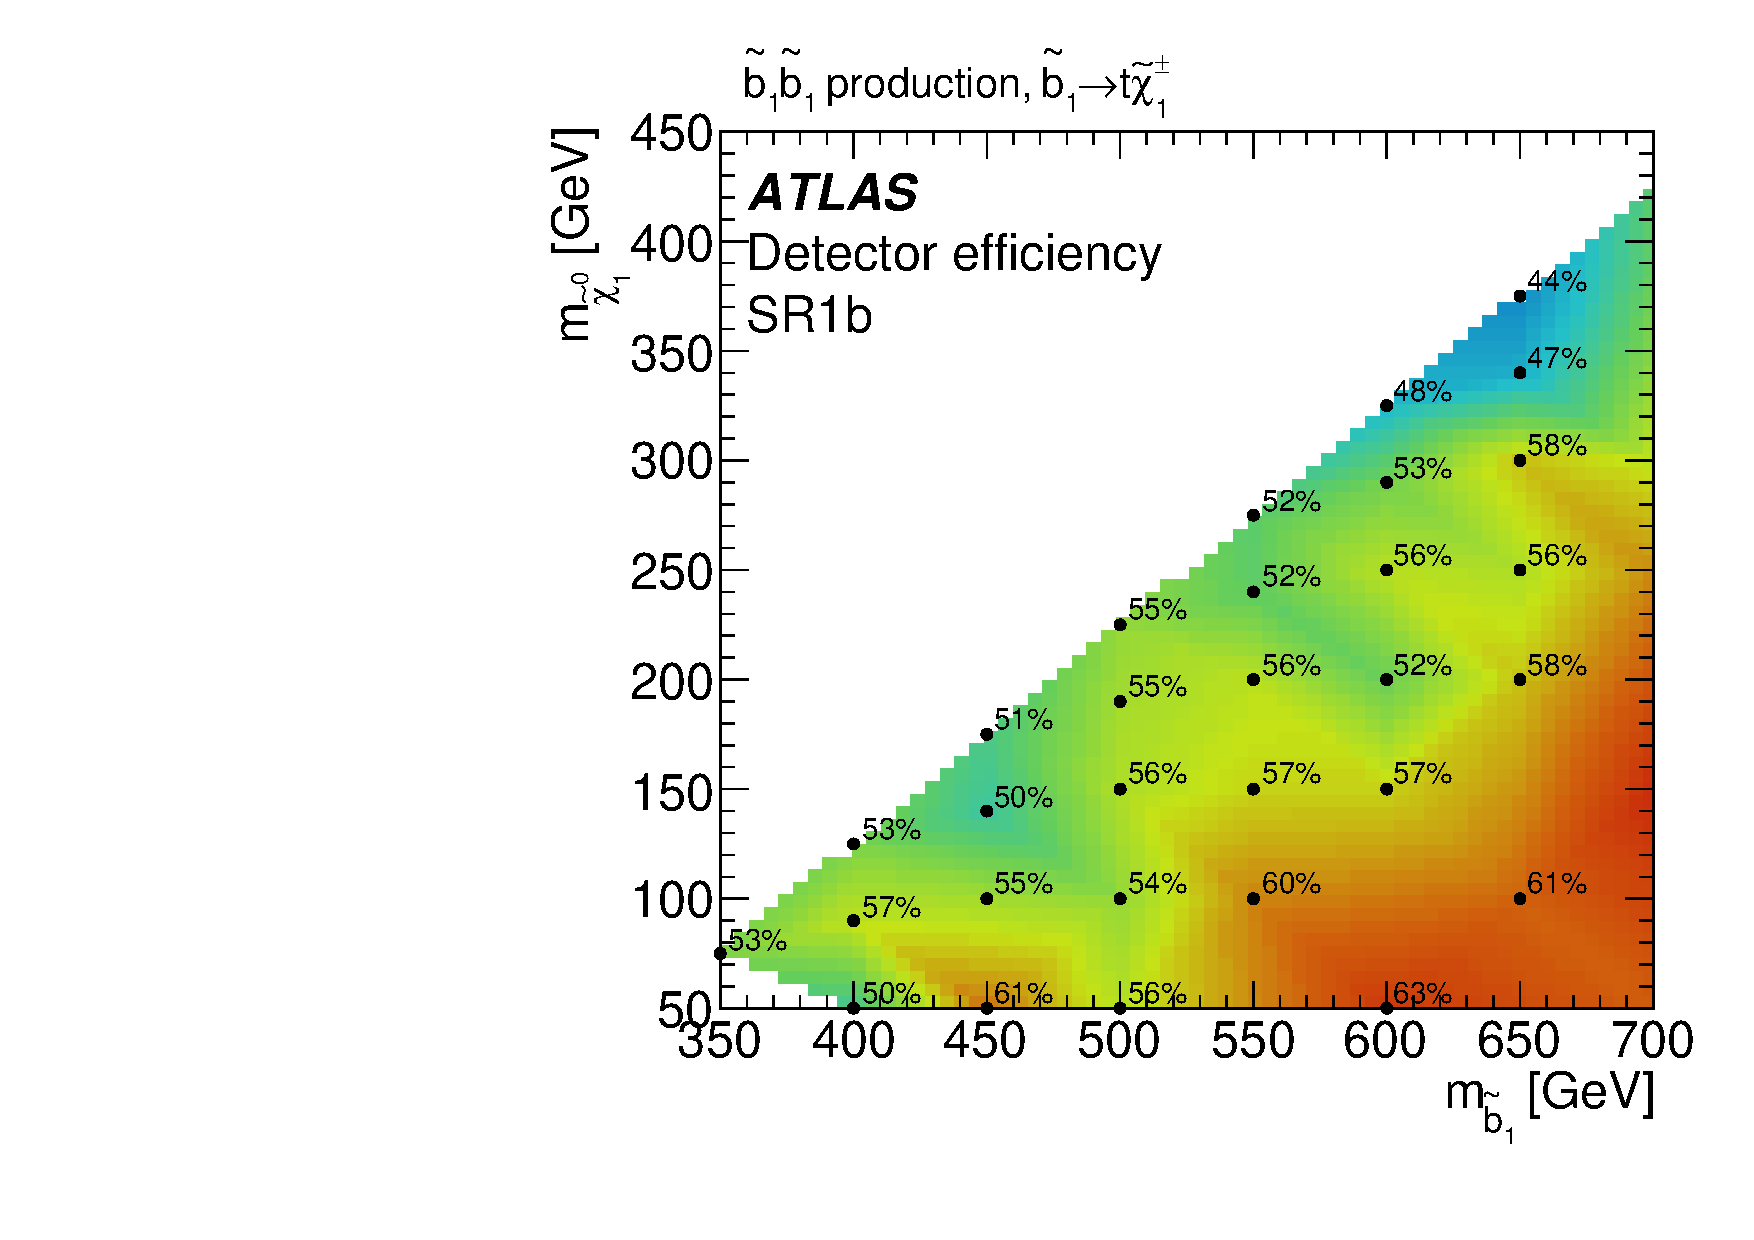
\includegraphics[width=\textwidth]{HEPDATA/efficiency_SR1b.pdf}
\caption{}\label{fig:hepdata_SR1b_efficiency}\end{subfigure}
\begin{subfigure}[t]{0.42\textwidth}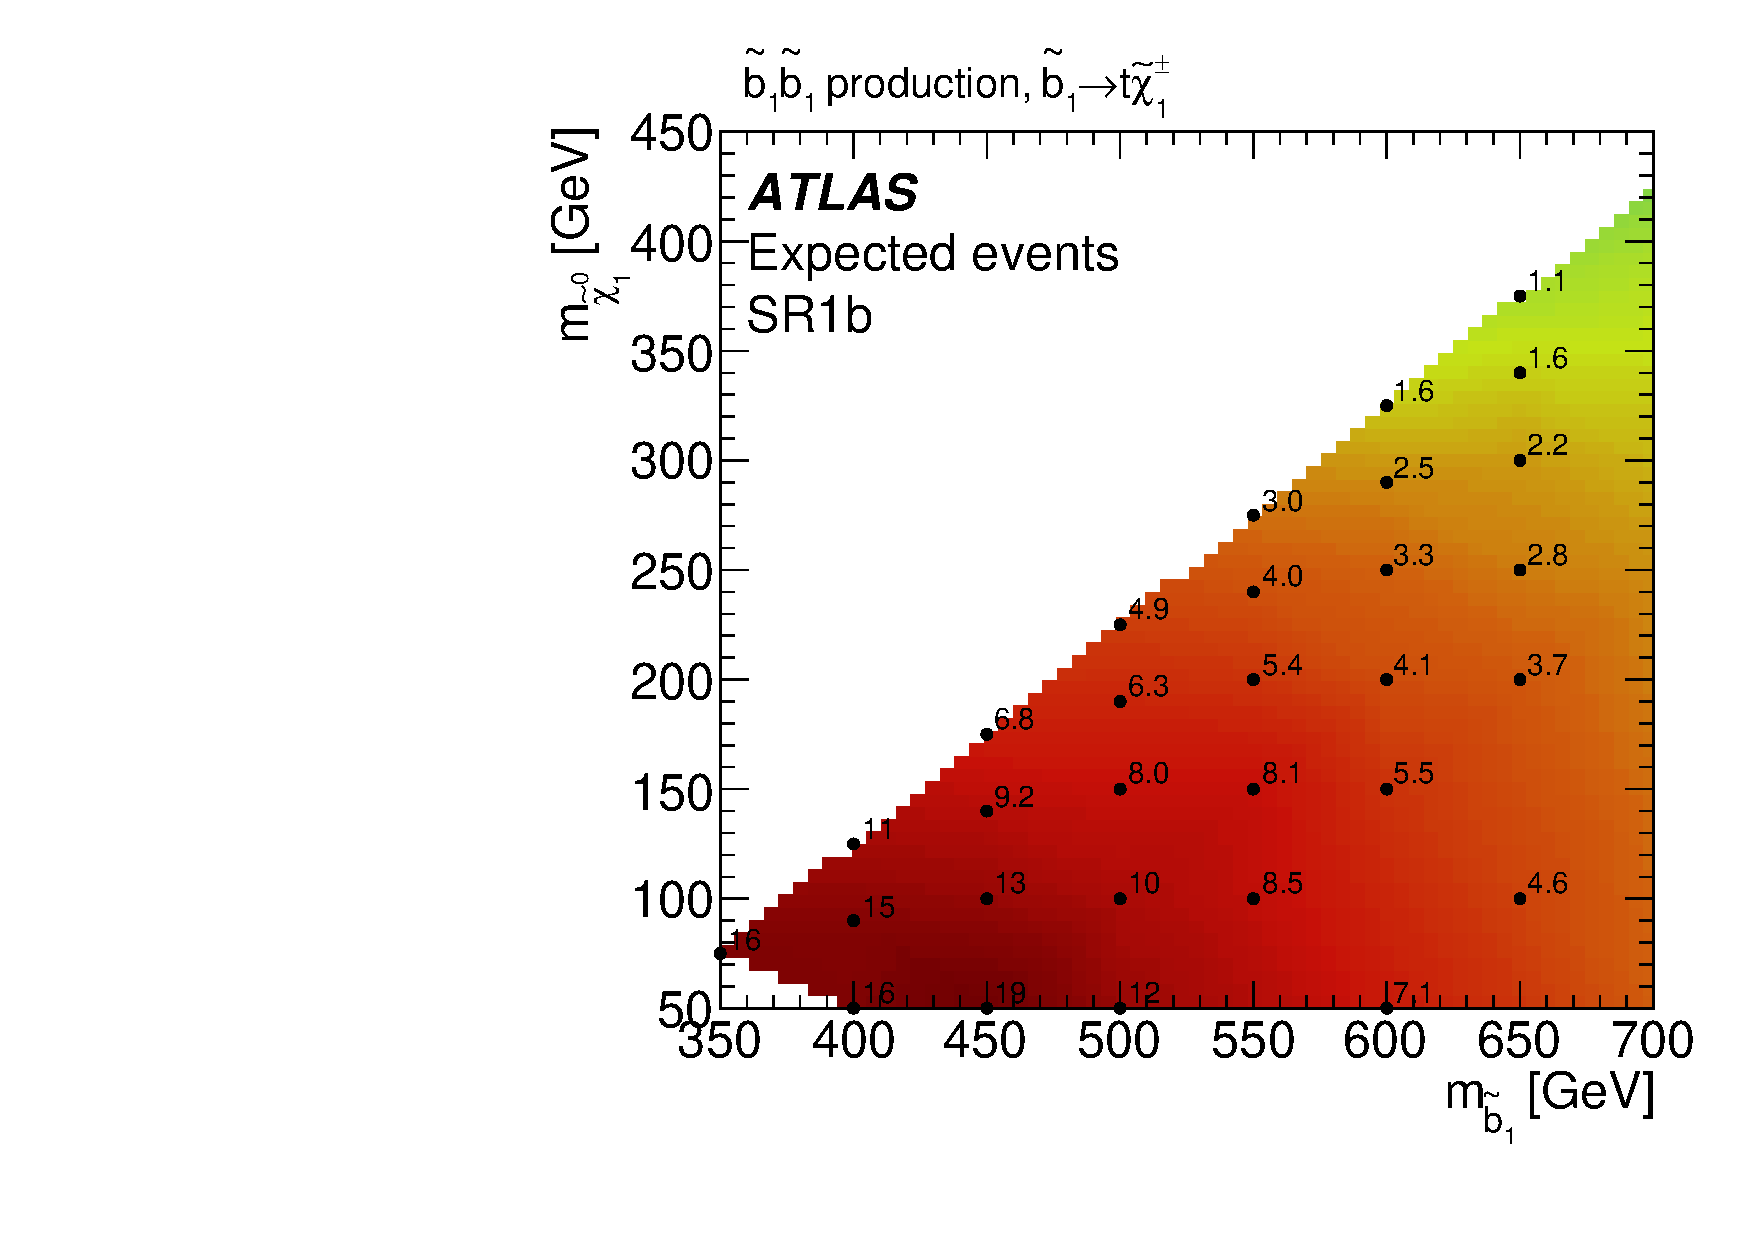
\includegraphics[width=\textwidth]{HEPDATA/yield_SR1b.pdf}
\caption{}\label{fig:hepdata_SR1b_yield}\end{subfigure}
\begin{subfigure}[t]{0.42\textwidth}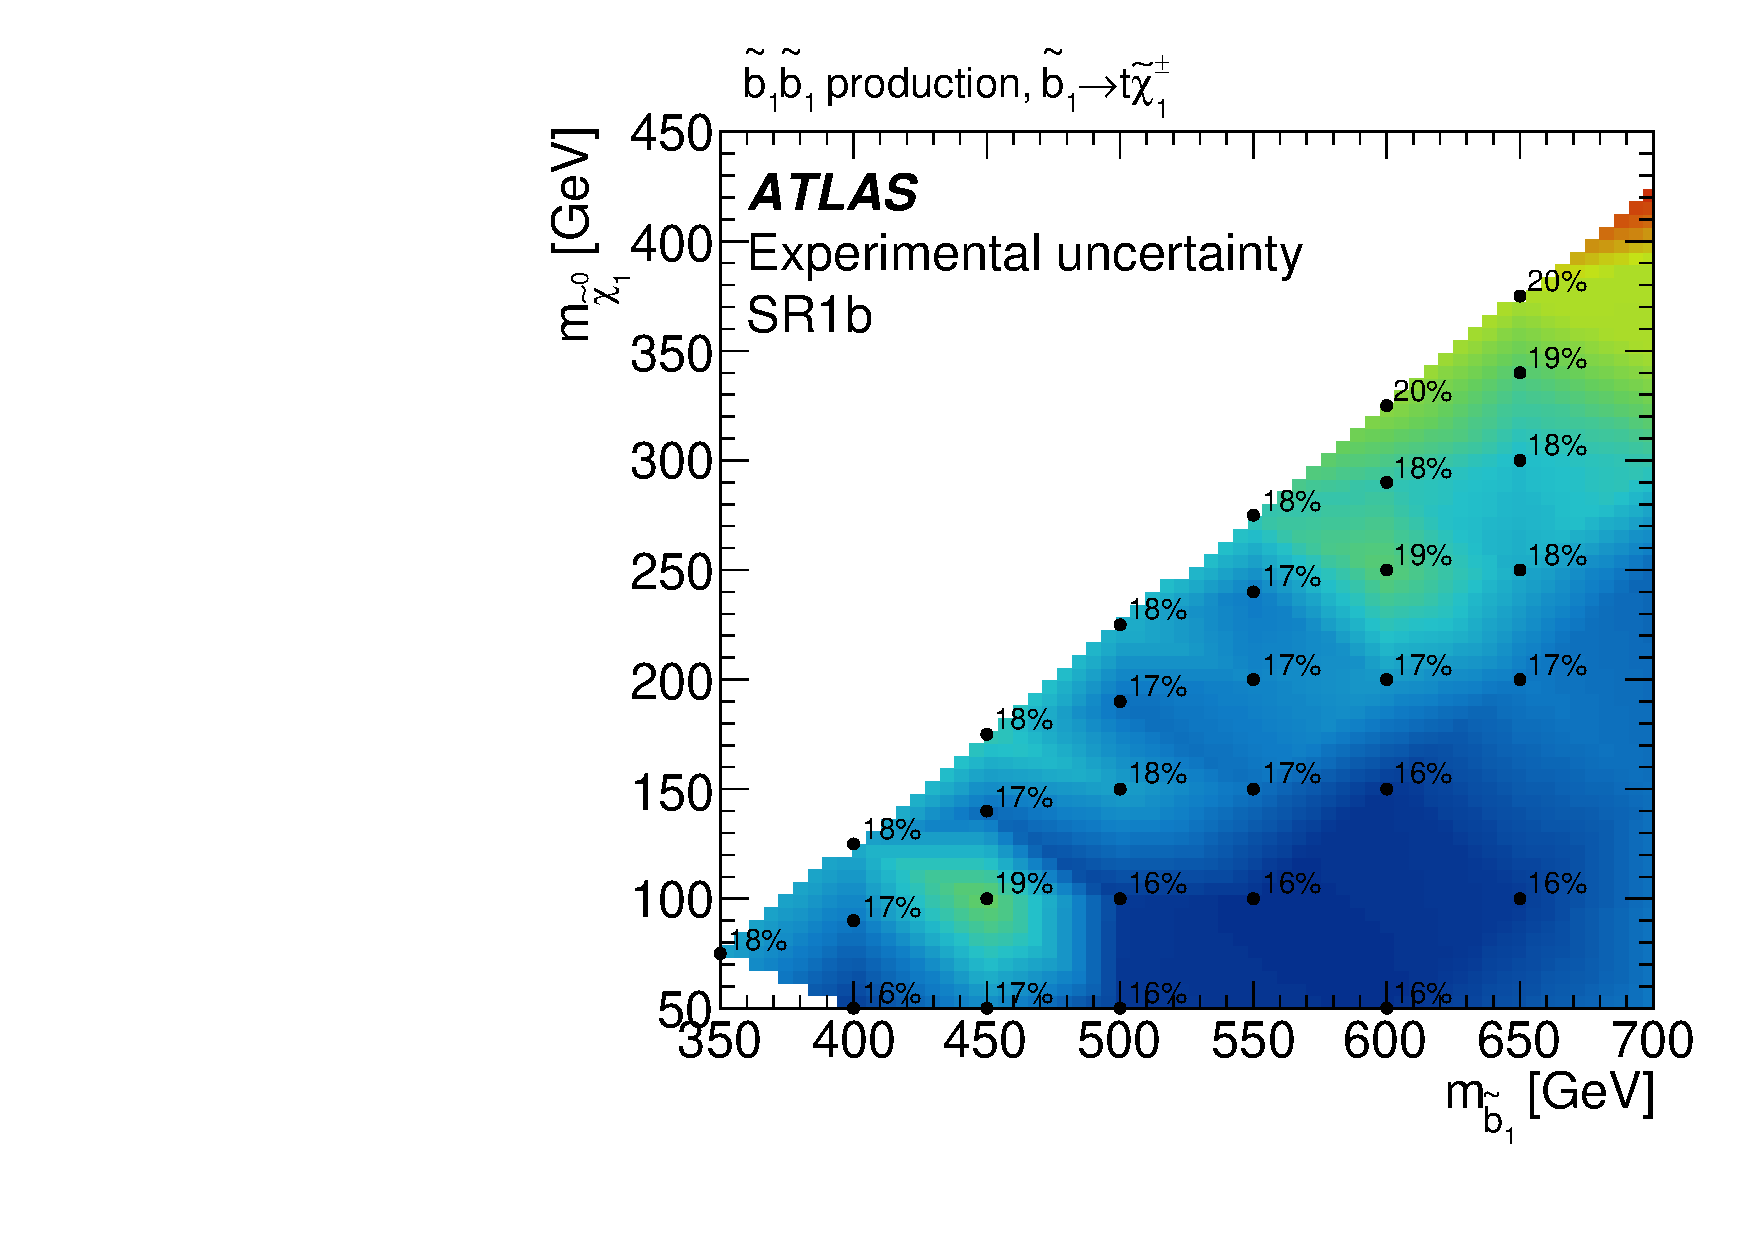
\includegraphics[width=\textwidth]{HEPDATA/mcsyst_SR1b.pdf}
\caption{}\label{fig:hepdata_SR1b_mcsyst}\end{subfigure}
\caption{SUSY scenario with $\sbottomone\sbottomone$ production and $\sbottomone\to tW\ninoone$ decay: 
(a) production cross-section, (b) number of generated MC events, 
(c) signal acceptance and (d) reconstruction efficiency in the signal region SR1b, 
(e) corresponding expected signal yield and (f) associated uncertainty due to experimental sources. 
The benchmark scenarios used to set exclusion limits are materialized by black dot markers. 
Acceptance and efficiency are defined as in appendix~A of~\cite{Stop2L}.}
\label{fig:HepData_SR1b} 
\end{figure}

\begin{figure}[p]
\centering
\begin{subfigure}[t]{0.42\textwidth}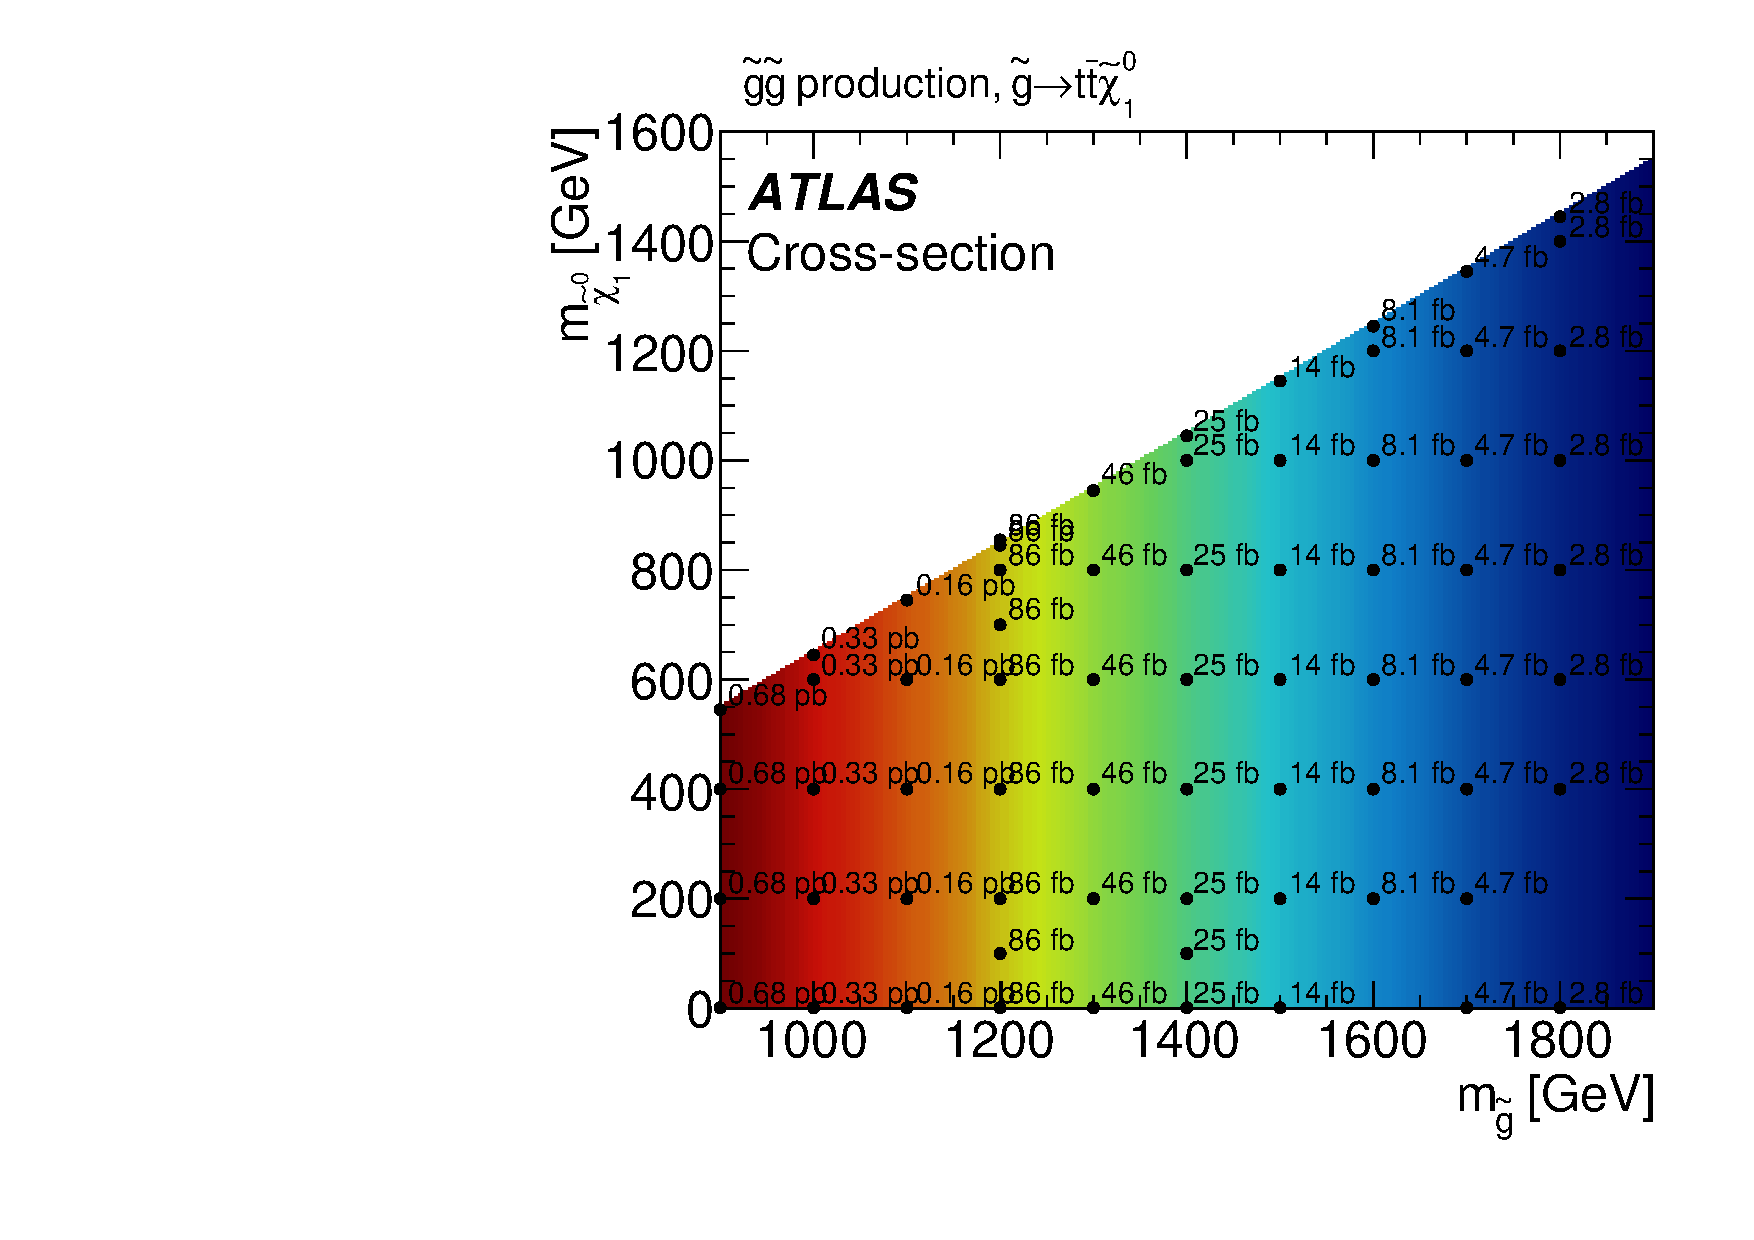
\includegraphics[width=\textwidth]{HEPDATA/xsection_SR3b.pdf}
\caption{}\label{fig:hepdata_SR3b_xsection}\end{subfigure}
\begin{subfigure}[t]{0.42\textwidth}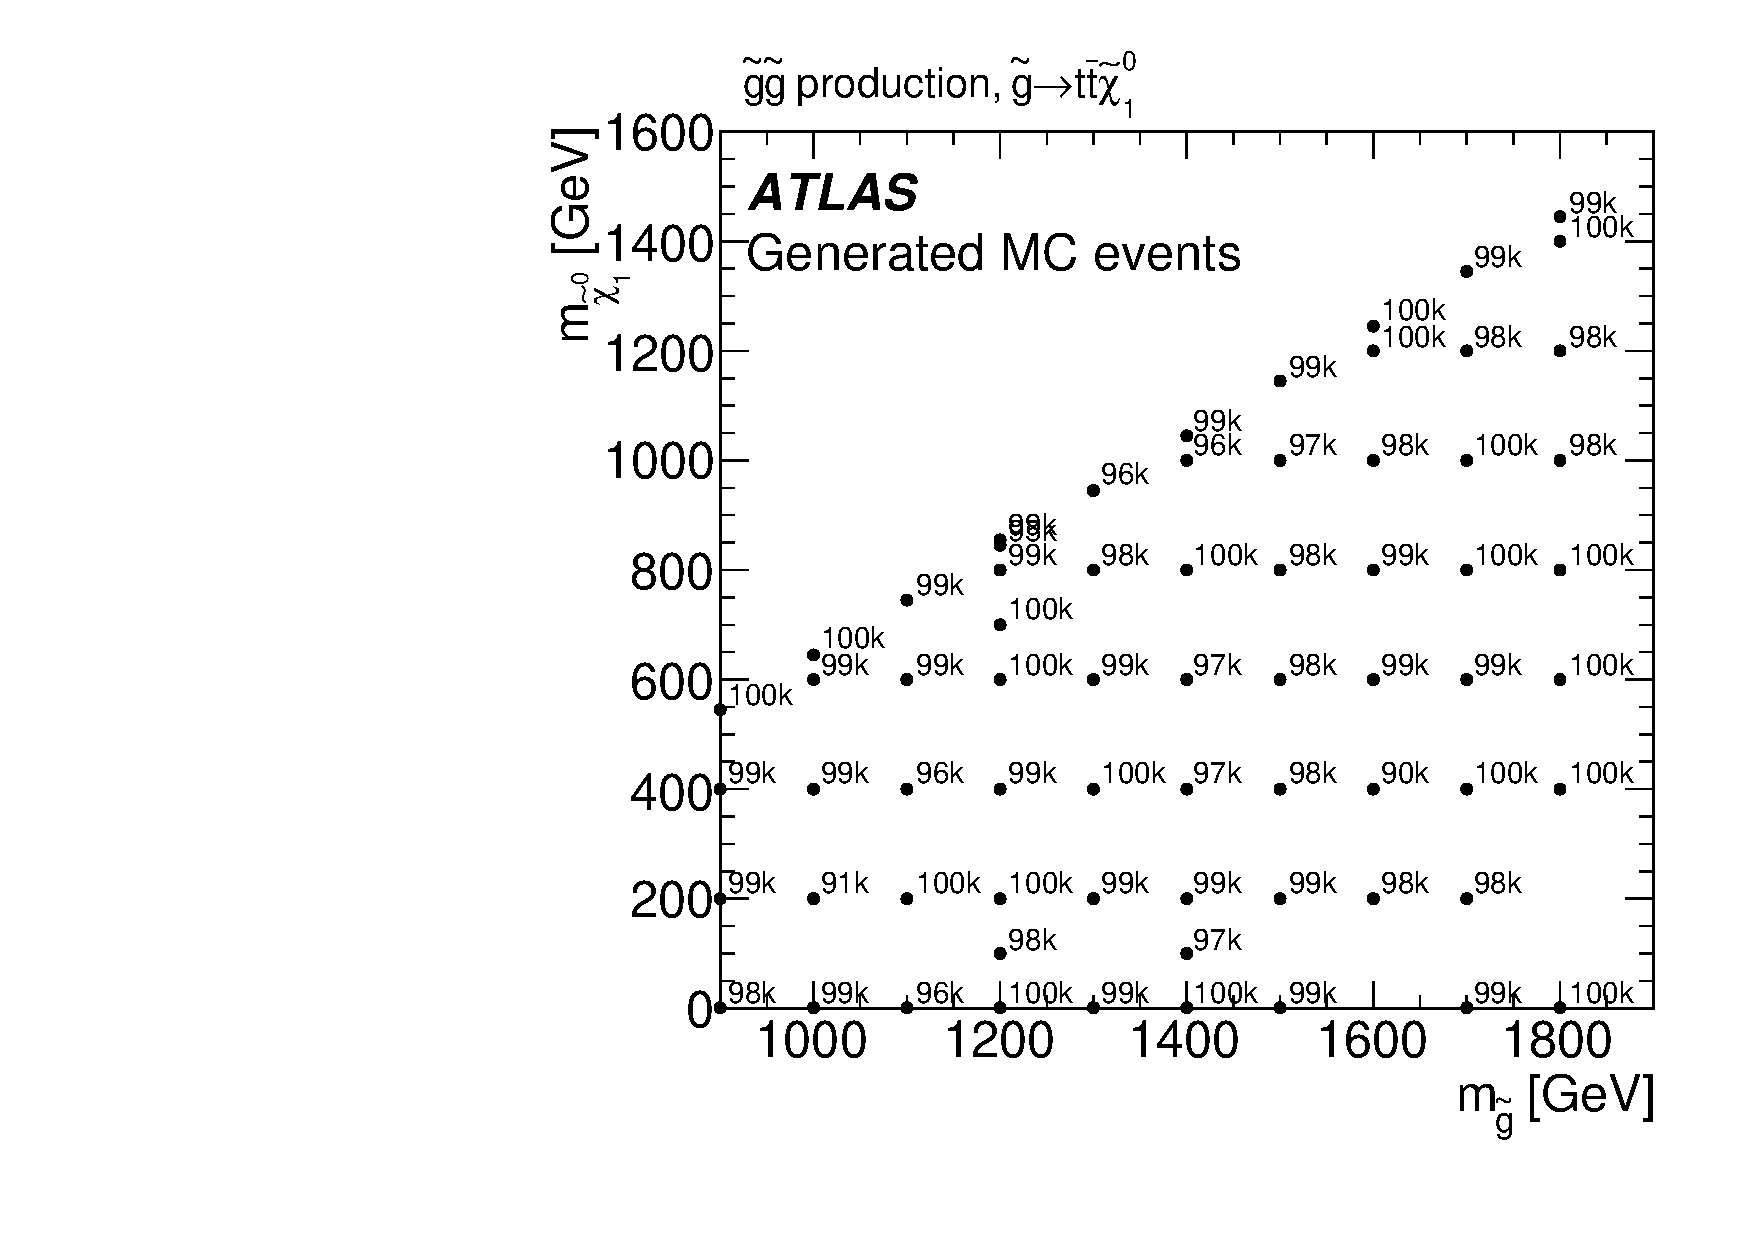
\includegraphics[width=\textwidth]{HEPDATA/mcstats_SR3b.pdf}
\caption{}\label{fig:hepdata_SR3b_mcstats}\end{subfigure}
\begin{subfigure}[t]{0.42\textwidth}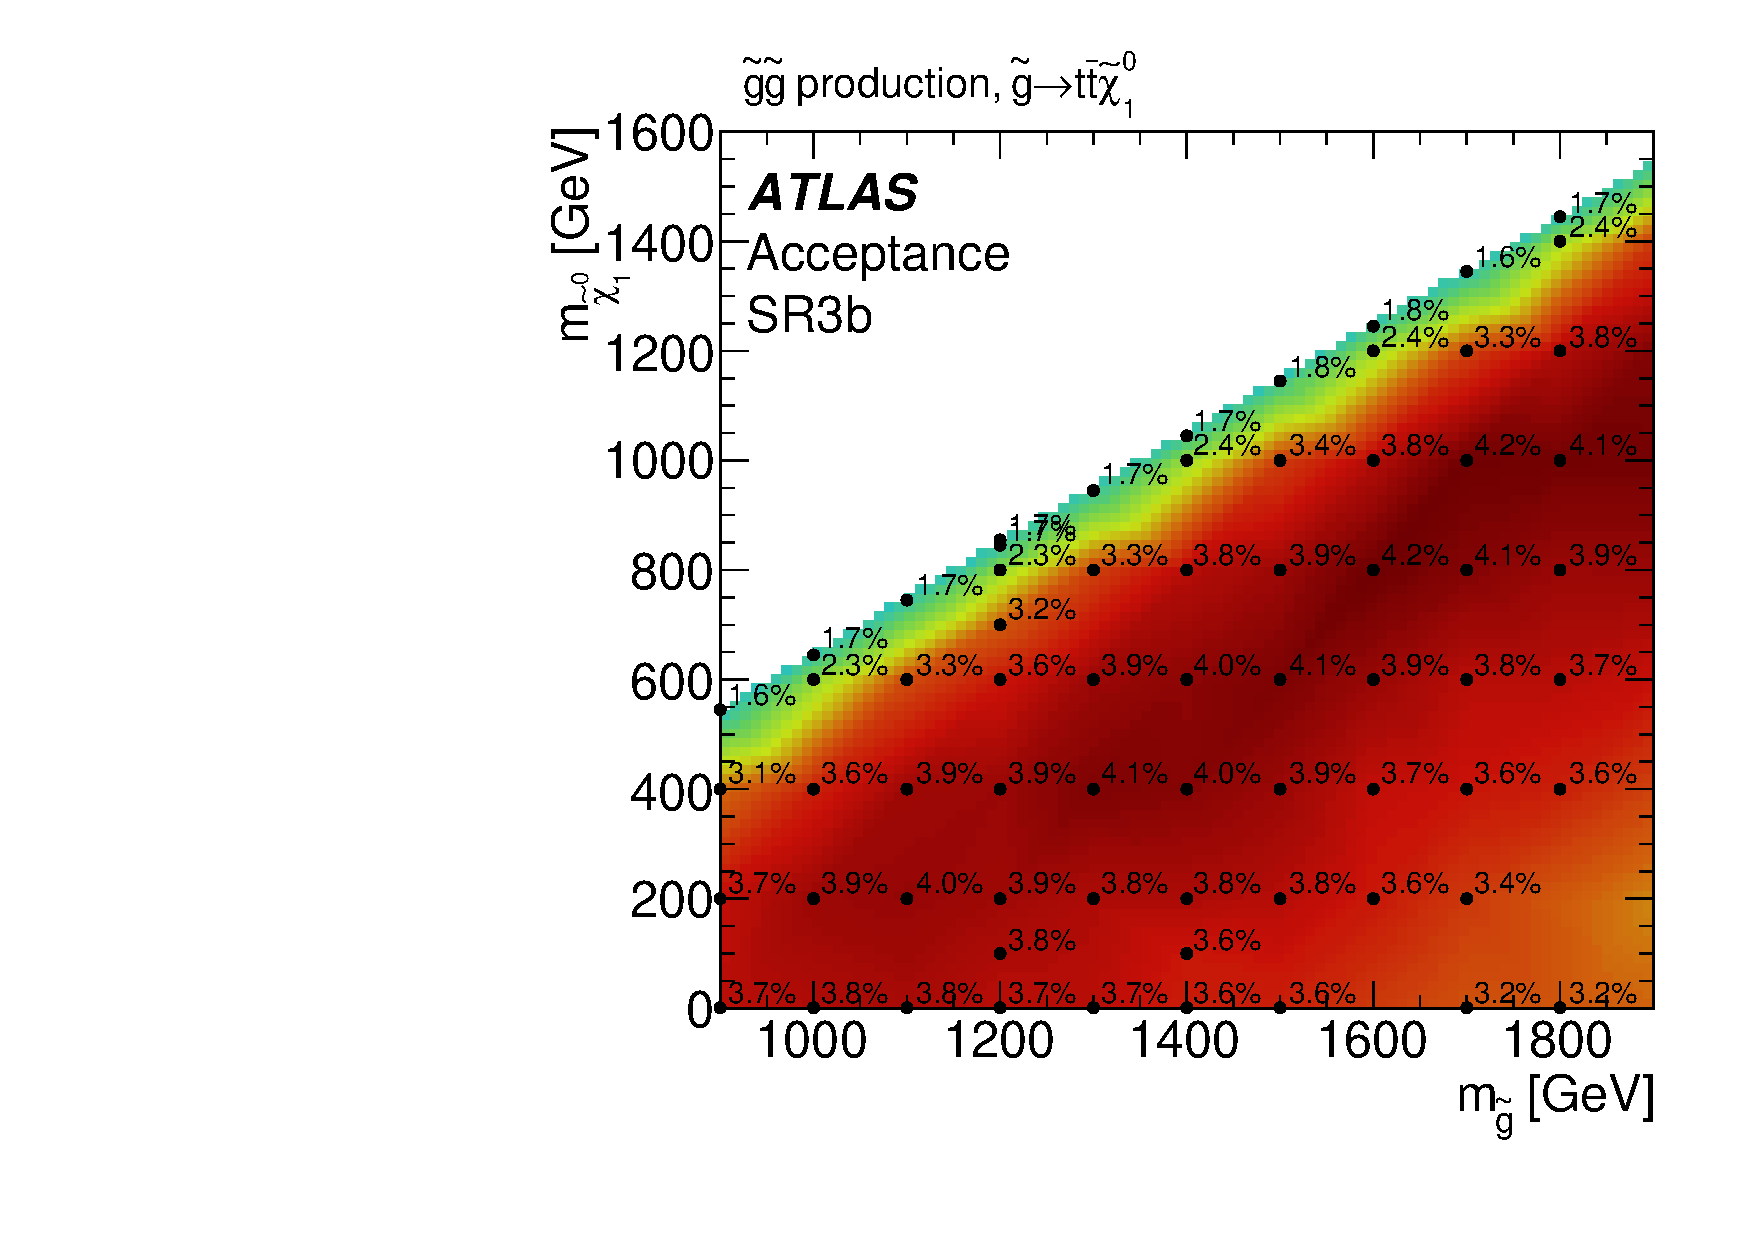
\includegraphics[width=\textwidth]{HEPDATA/acceptance_SR3b.pdf}
\caption{}\label{fig:hepdata_SR3b_acceptance}\end{subfigure}
\begin{subfigure}[t]{0.42\textwidth}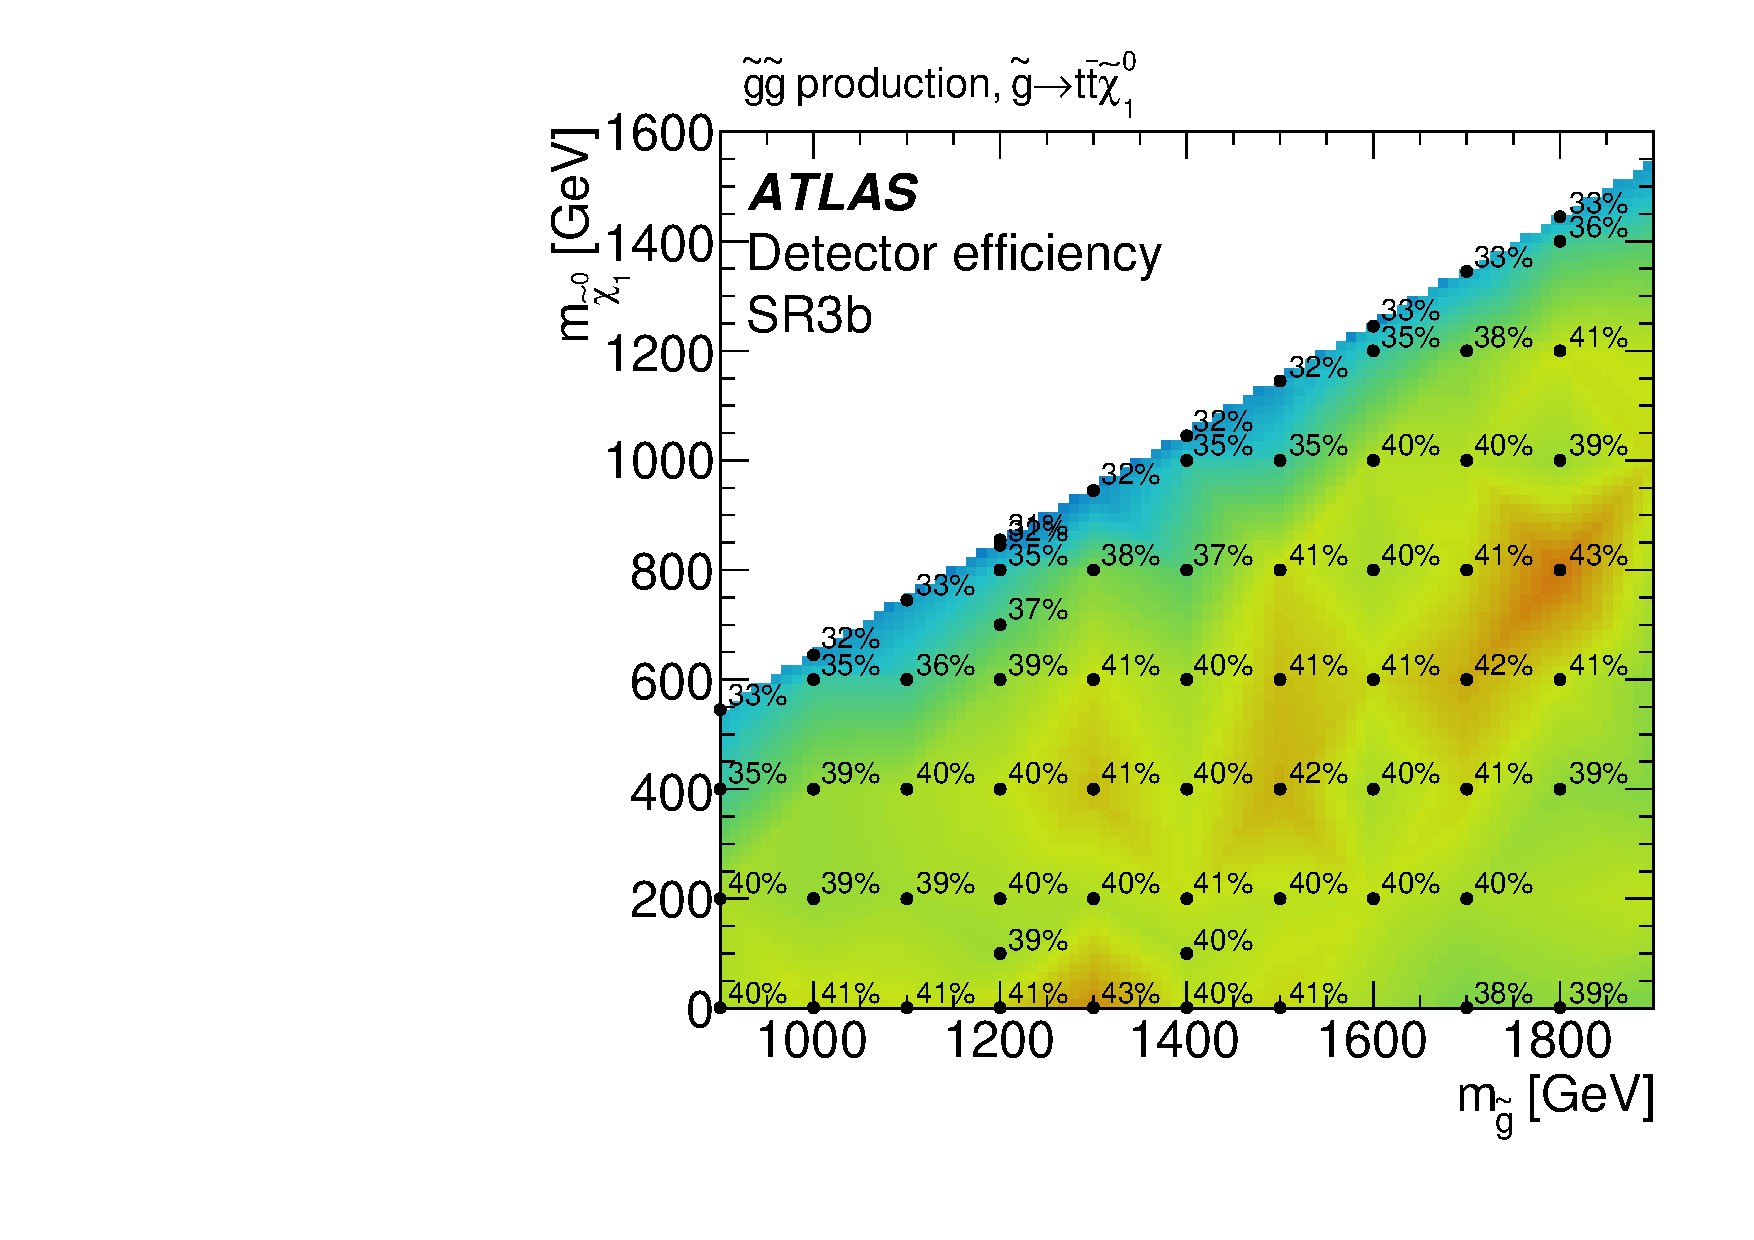
\includegraphics[width=\textwidth]{HEPDATA/efficiency_SR3b.pdf}
\caption{}\label{fig:hepdata_SR3b_efficiency}\end{subfigure}
\begin{subfigure}[t]{0.42\textwidth}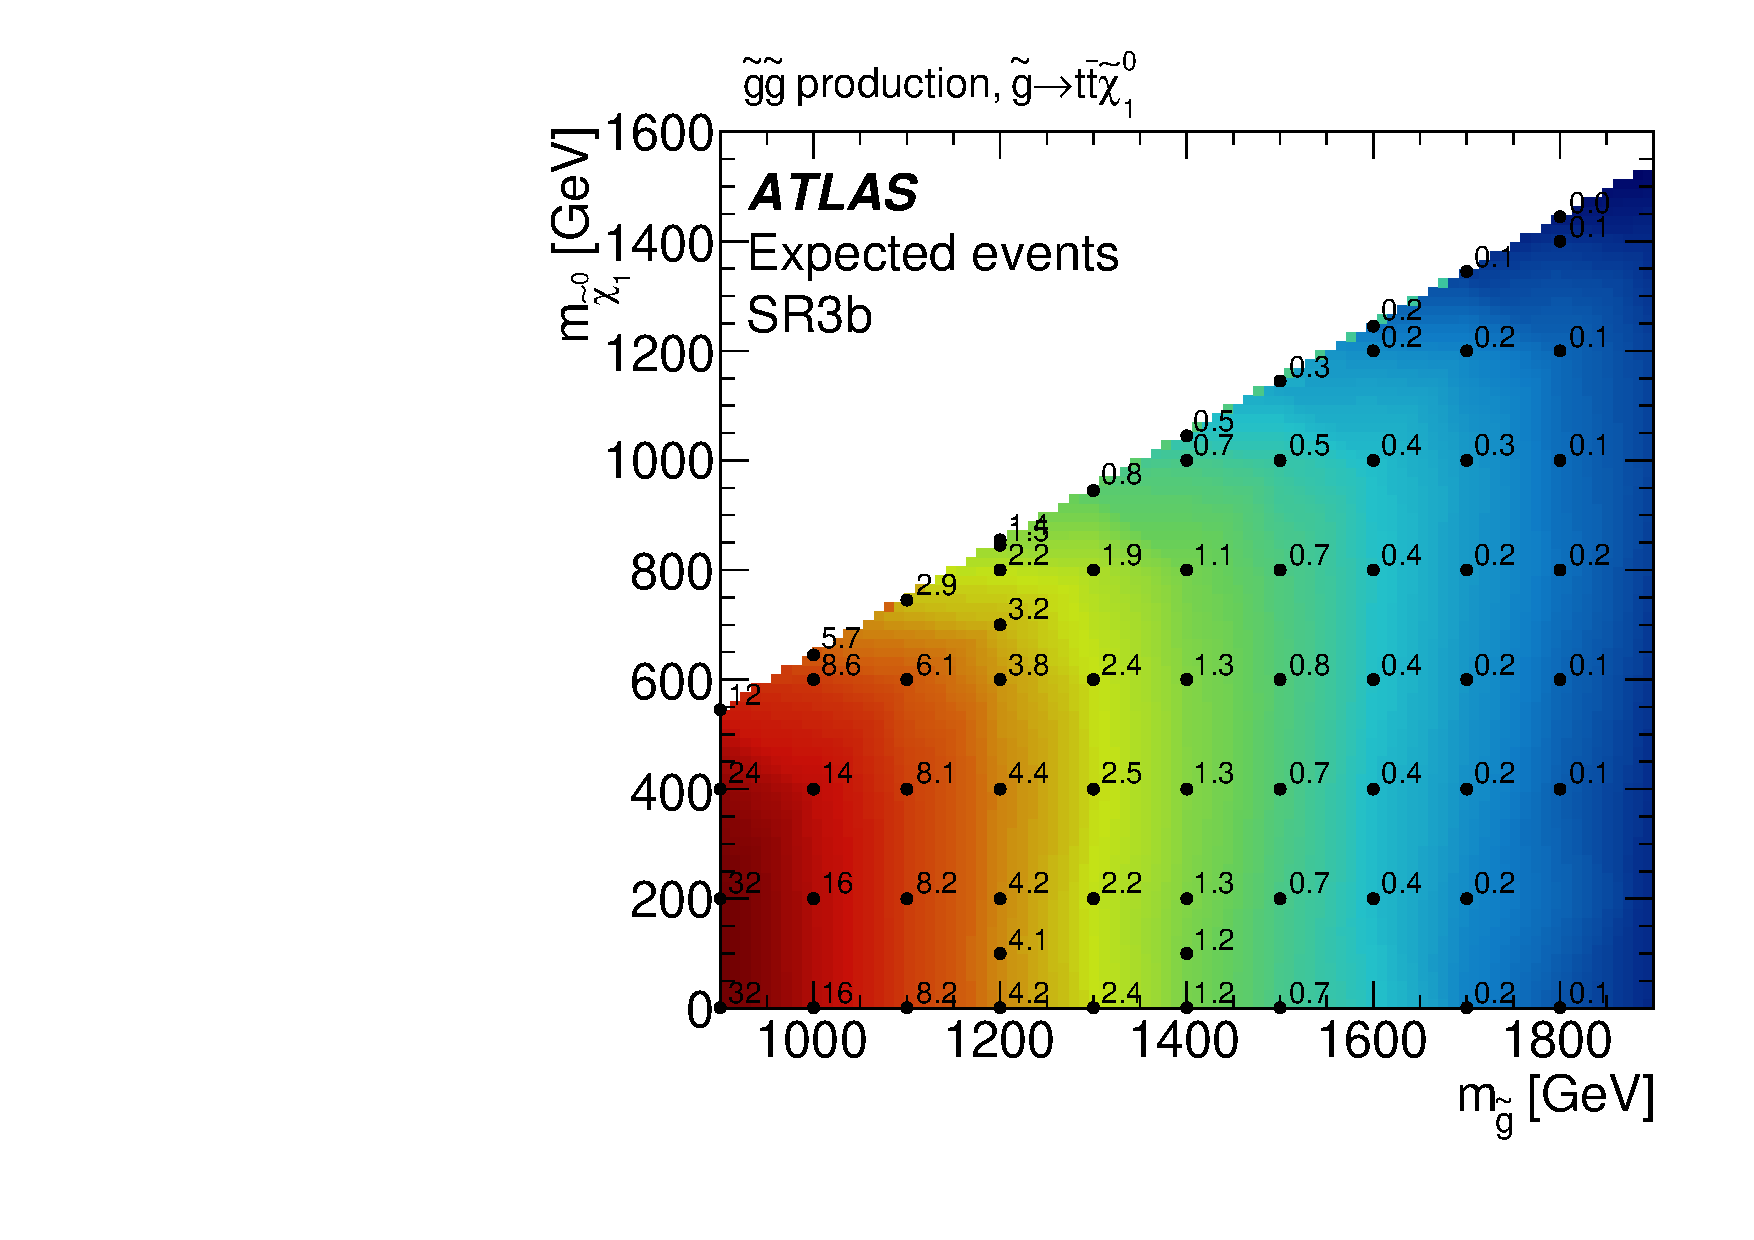
\includegraphics[width=\textwidth]{HEPDATA/yield_SR3b.pdf}
\caption{}\label{fig:hepdata_SR3b_yield}\end{subfigure}
\begin{subfigure}[t]{0.42\textwidth}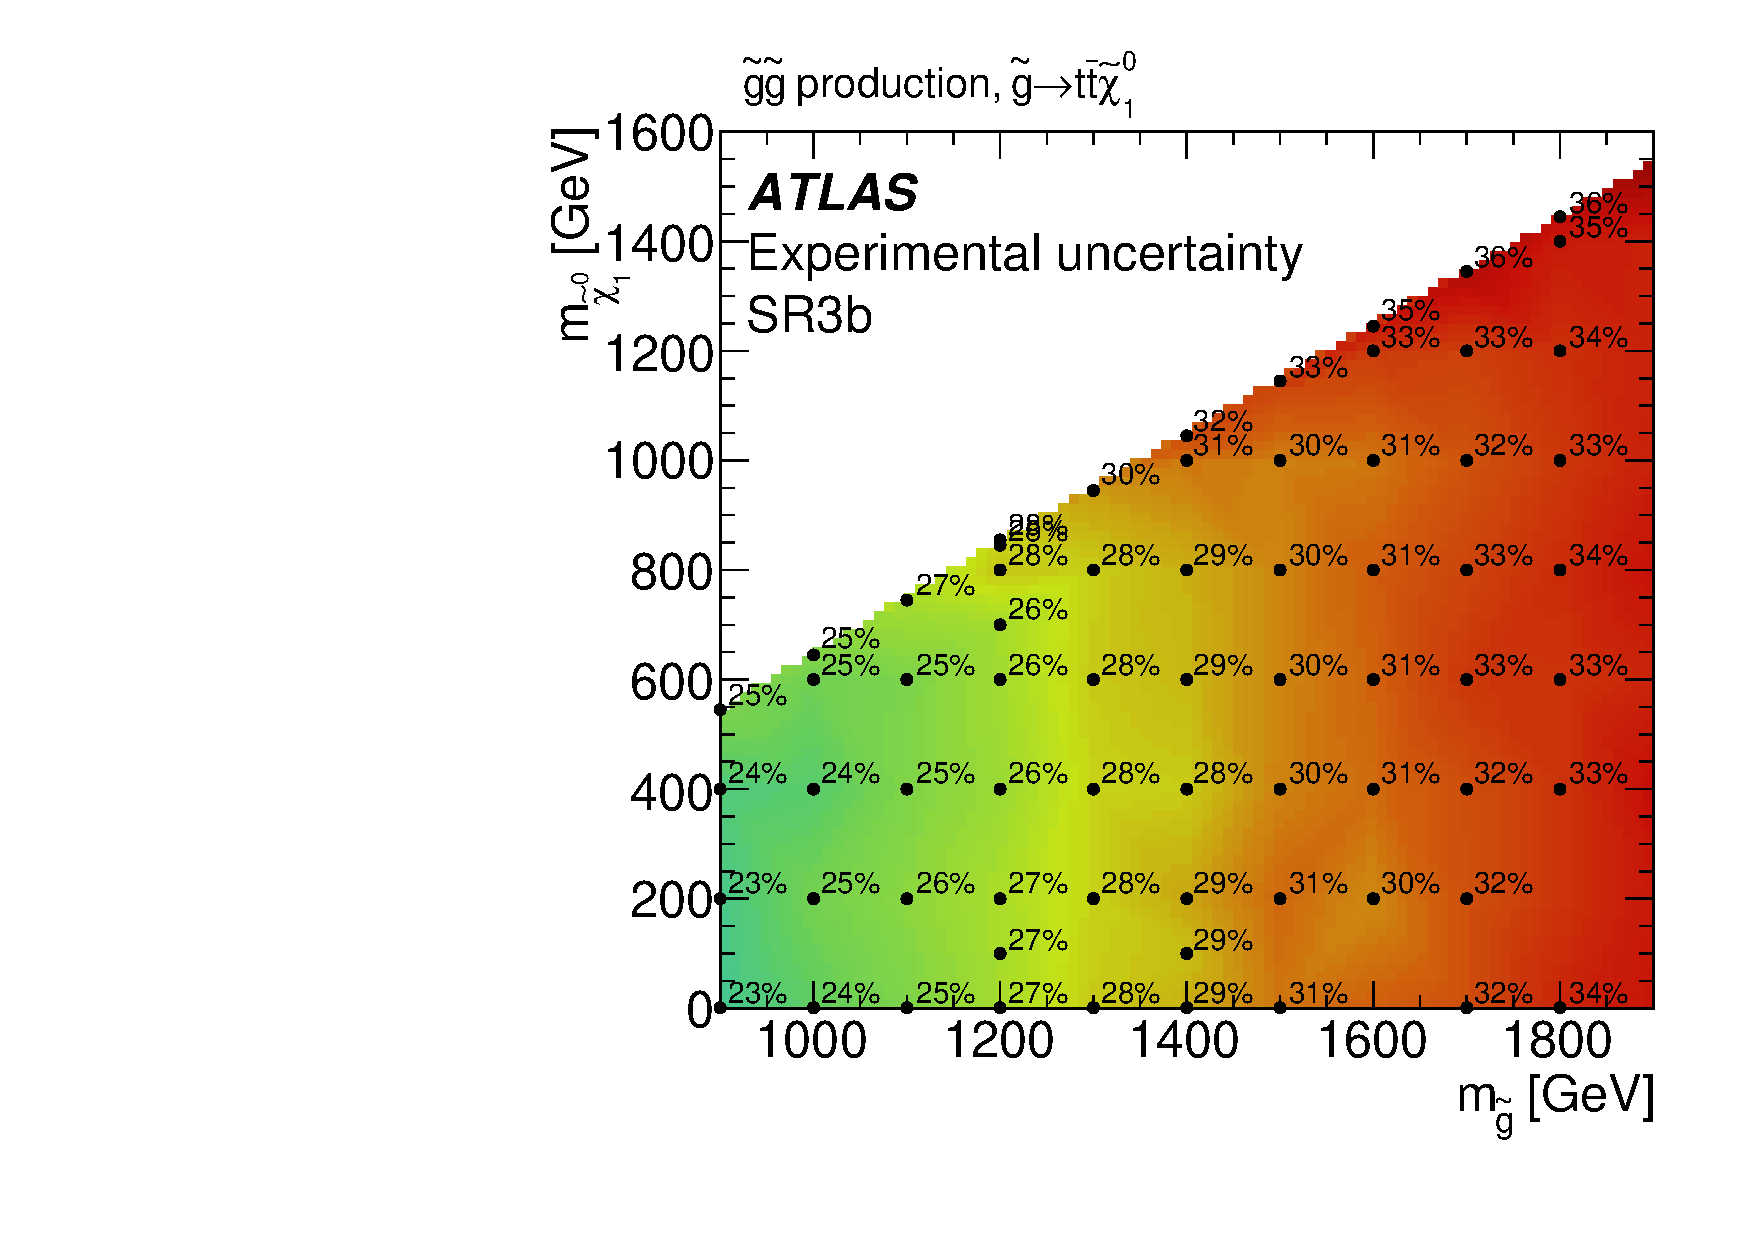
\includegraphics[width=\textwidth]{HEPDATA/mcsyst_SR3b.pdf}
\caption{}\label{fig:hepdata_SR3b_mcsyst}\end{subfigure}
\caption{SUSY scenario with $\gluino\gluino$ production and $\gluino\to t\bar t\ninoone$ decay: 
(a) production cross-section, (b) number of generated MC events, 
(c) signal acceptance and (d) reconstruction efficiency in the signal region SR3b, 
(e) corresponding expected signal yield and (f) associated uncertainty due to experimental sources. 
The benchmark scenarios used to set exclusion limits are materialized by black dot markers. 
Acceptance and efficiency are defined as in appendix~A of~\cite{Stop2L}.}
\label{fig:HepData_SR3b} 
\end{figure} 

\begin{figure}[p]
\centering
\begin{subfigure}[t]{0.42\textwidth}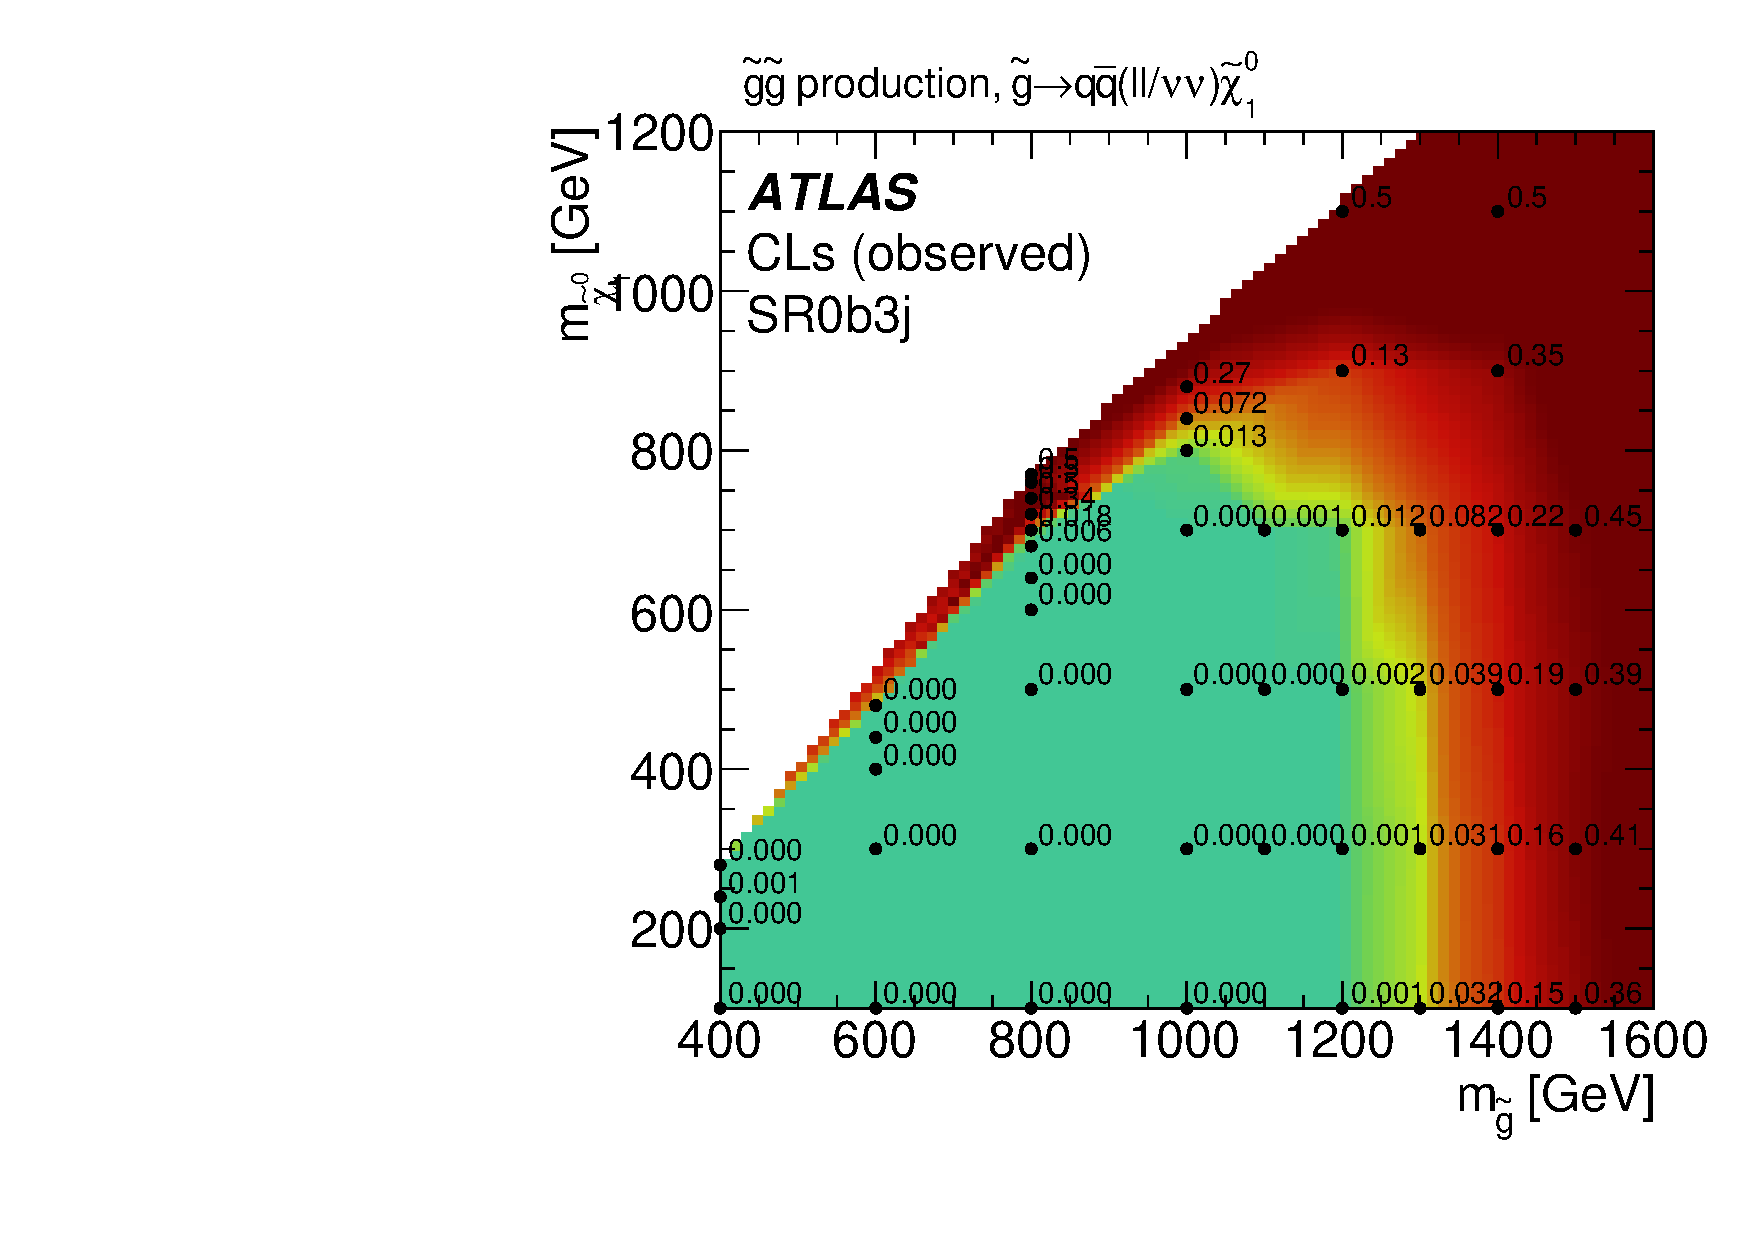
\includegraphics[width=\textwidth]{HEPDATA/clobs_SR0b3j.pdf}
\caption{$\gluino\to q\bar q \ell\ell\ninoone$ scenario, SR0b3j}\label{fig:hepdata_SR0b3j_CLobs}\end{subfigure}
\begin{subfigure}[t]{0.42\textwidth}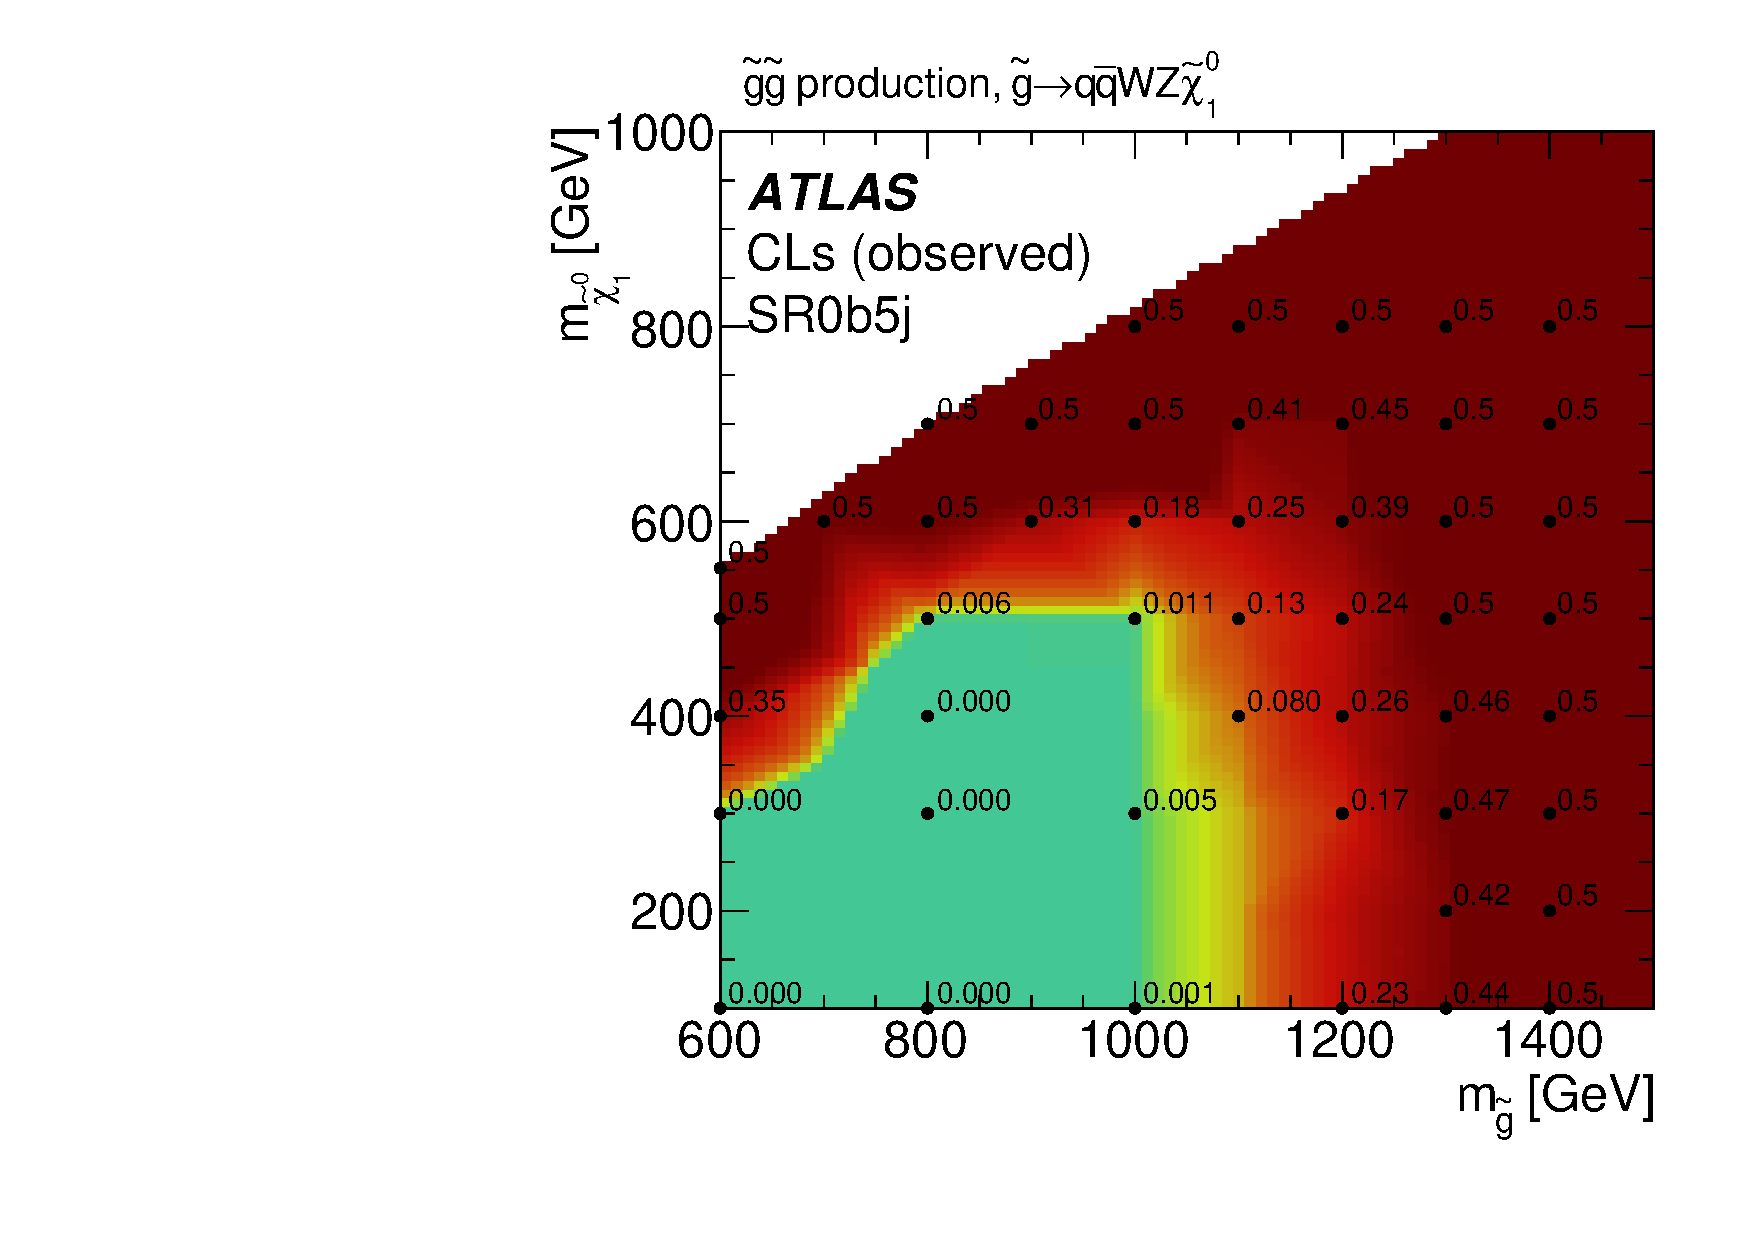
\includegraphics[width=\textwidth]{HEPDATA/clobs_SR0b5j.pdf}
\caption{$\gluino\to q\bar q' WZ\ninoone$ scenario, SR0b5j}\label{fig:hepdata_SR0b5j_CLobs}\end{subfigure}
\begin{subfigure}[t]{0.42\textwidth}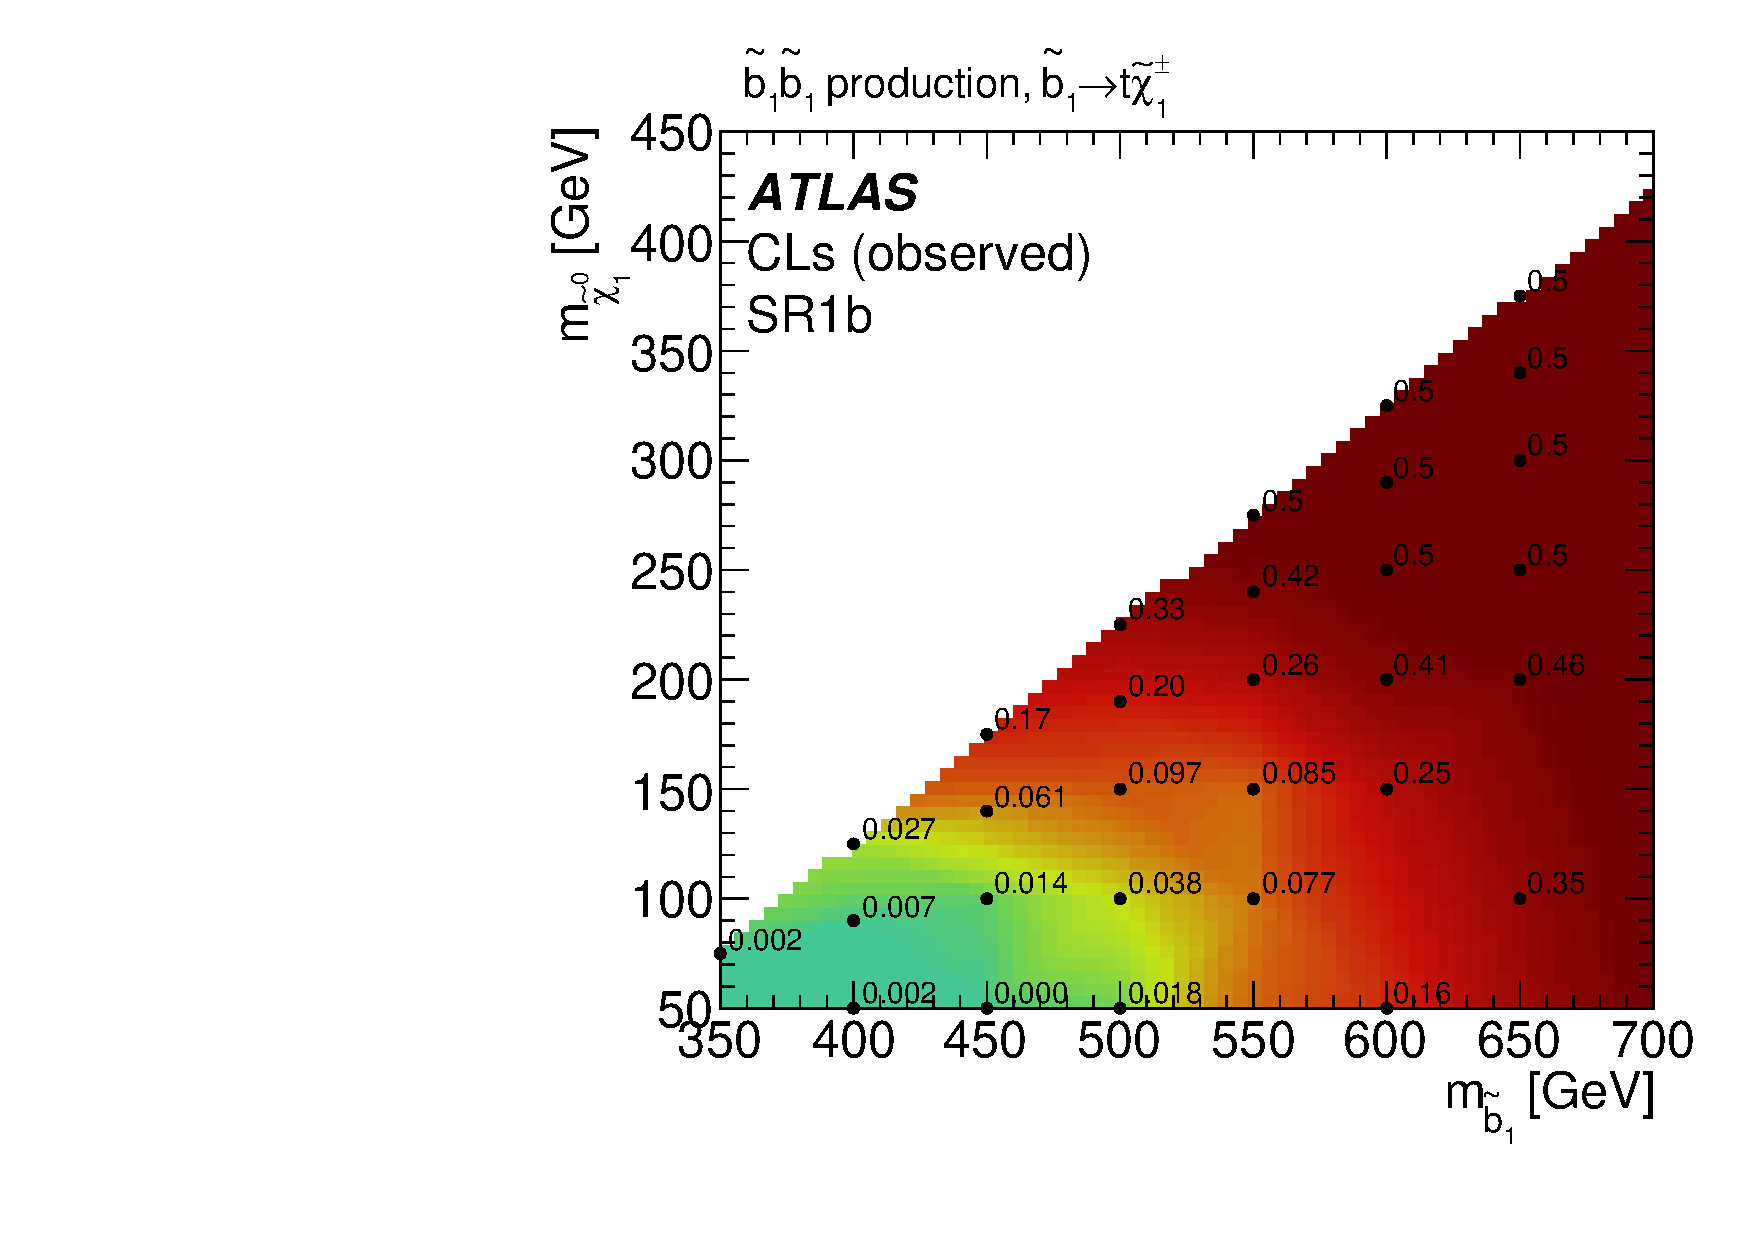
\includegraphics[width=\textwidth]{HEPDATA/clobs_SR1b.pdf}
\caption{$\sbottomone\to tW^-\ninoone$ scenario, SR1b}\label{fig:hepdata_SR1b_CLobs}\end{subfigure}
\begin{subfigure}[t]{0.42\textwidth}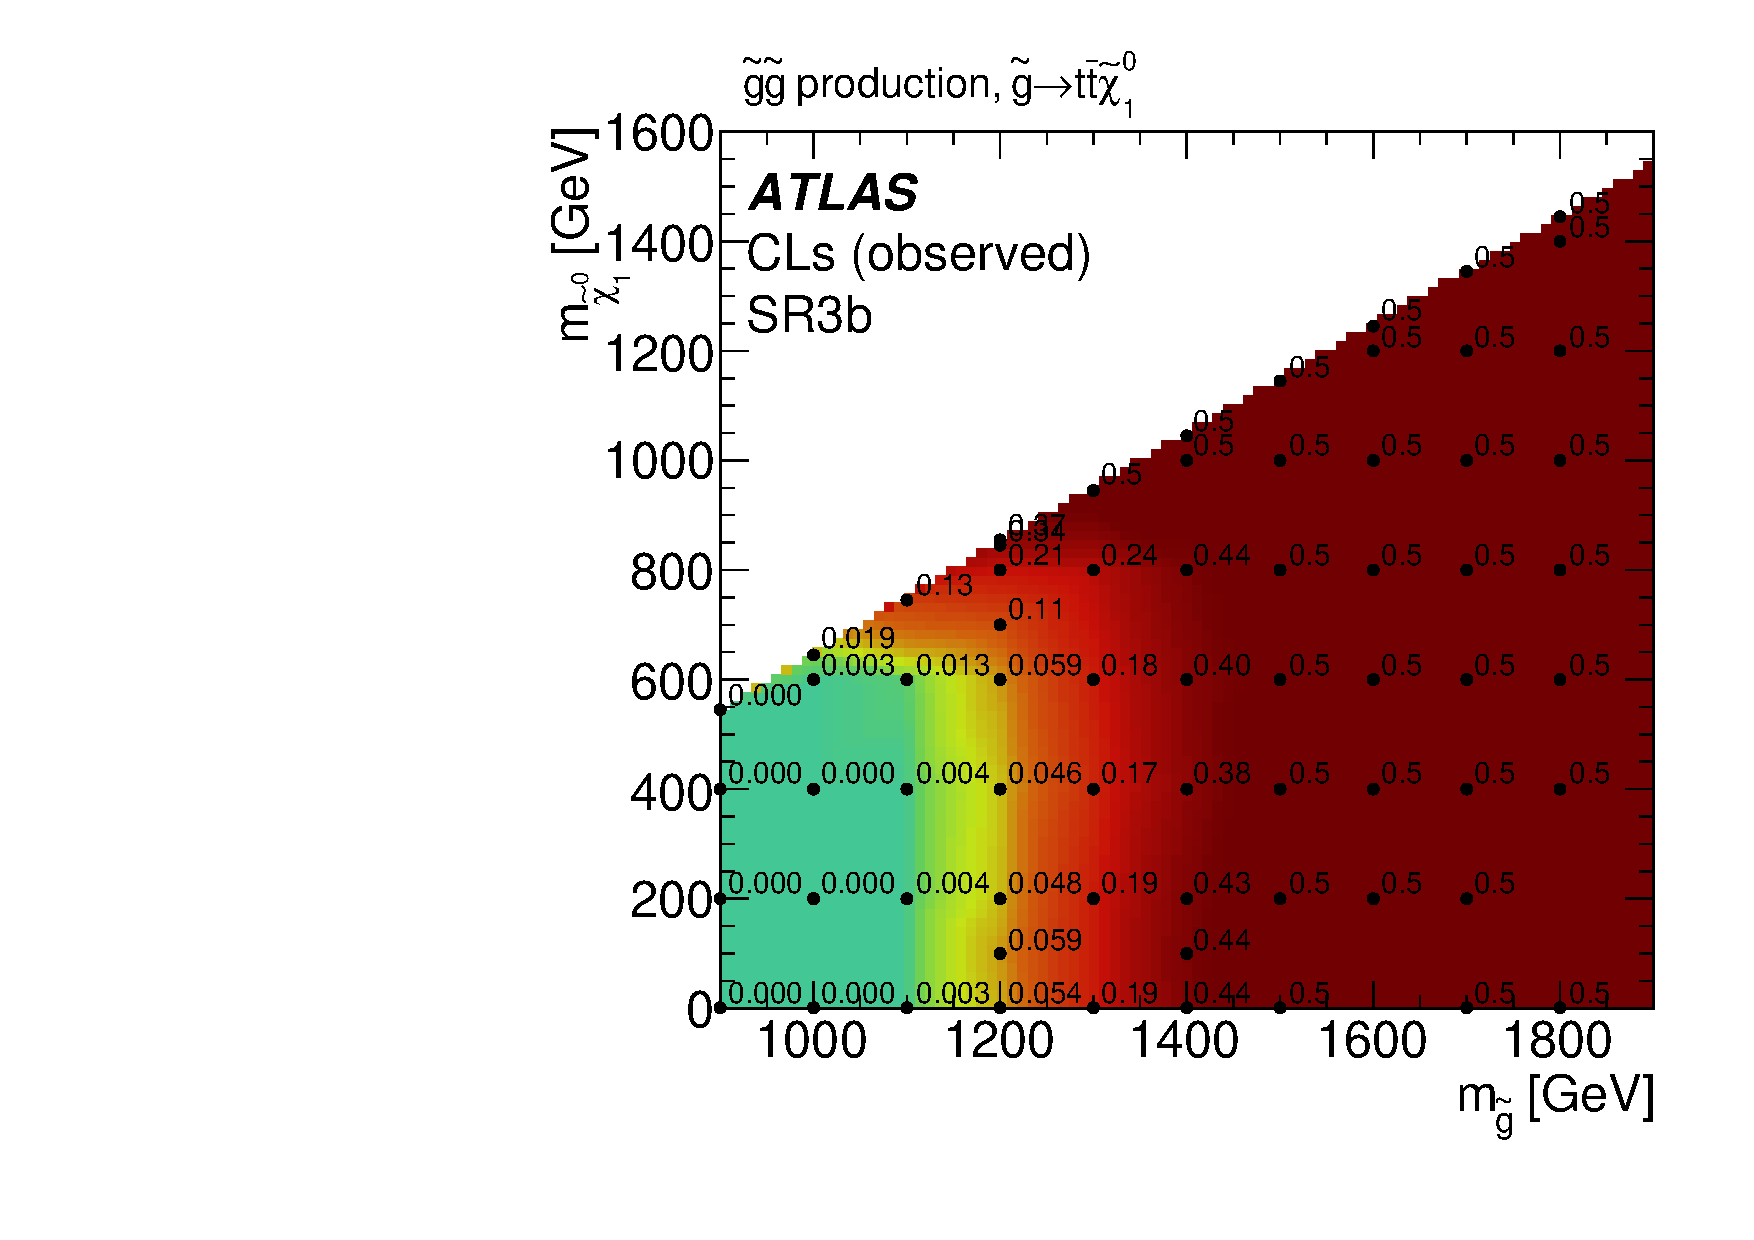
\includegraphics[width=\textwidth]{HEPDATA/clobs_SR3b.pdf}
\caption{$\gluino\to t\bar t\ninoone$ scenario, SR3b}\label{fig:hepdata_SR3b_CLobs}\end{subfigure}
\caption{Observed CL$_\mathrm{s}$ in the four signal regions. 
The benchmark scenarios used to set exclusion limits are materialized by black dot markers.}
\label{fig:HepData_CLobs} 
\end{figure} 

\begin{figure}[p]
\centering
\begin{subfigure}[t]{0.42\textwidth}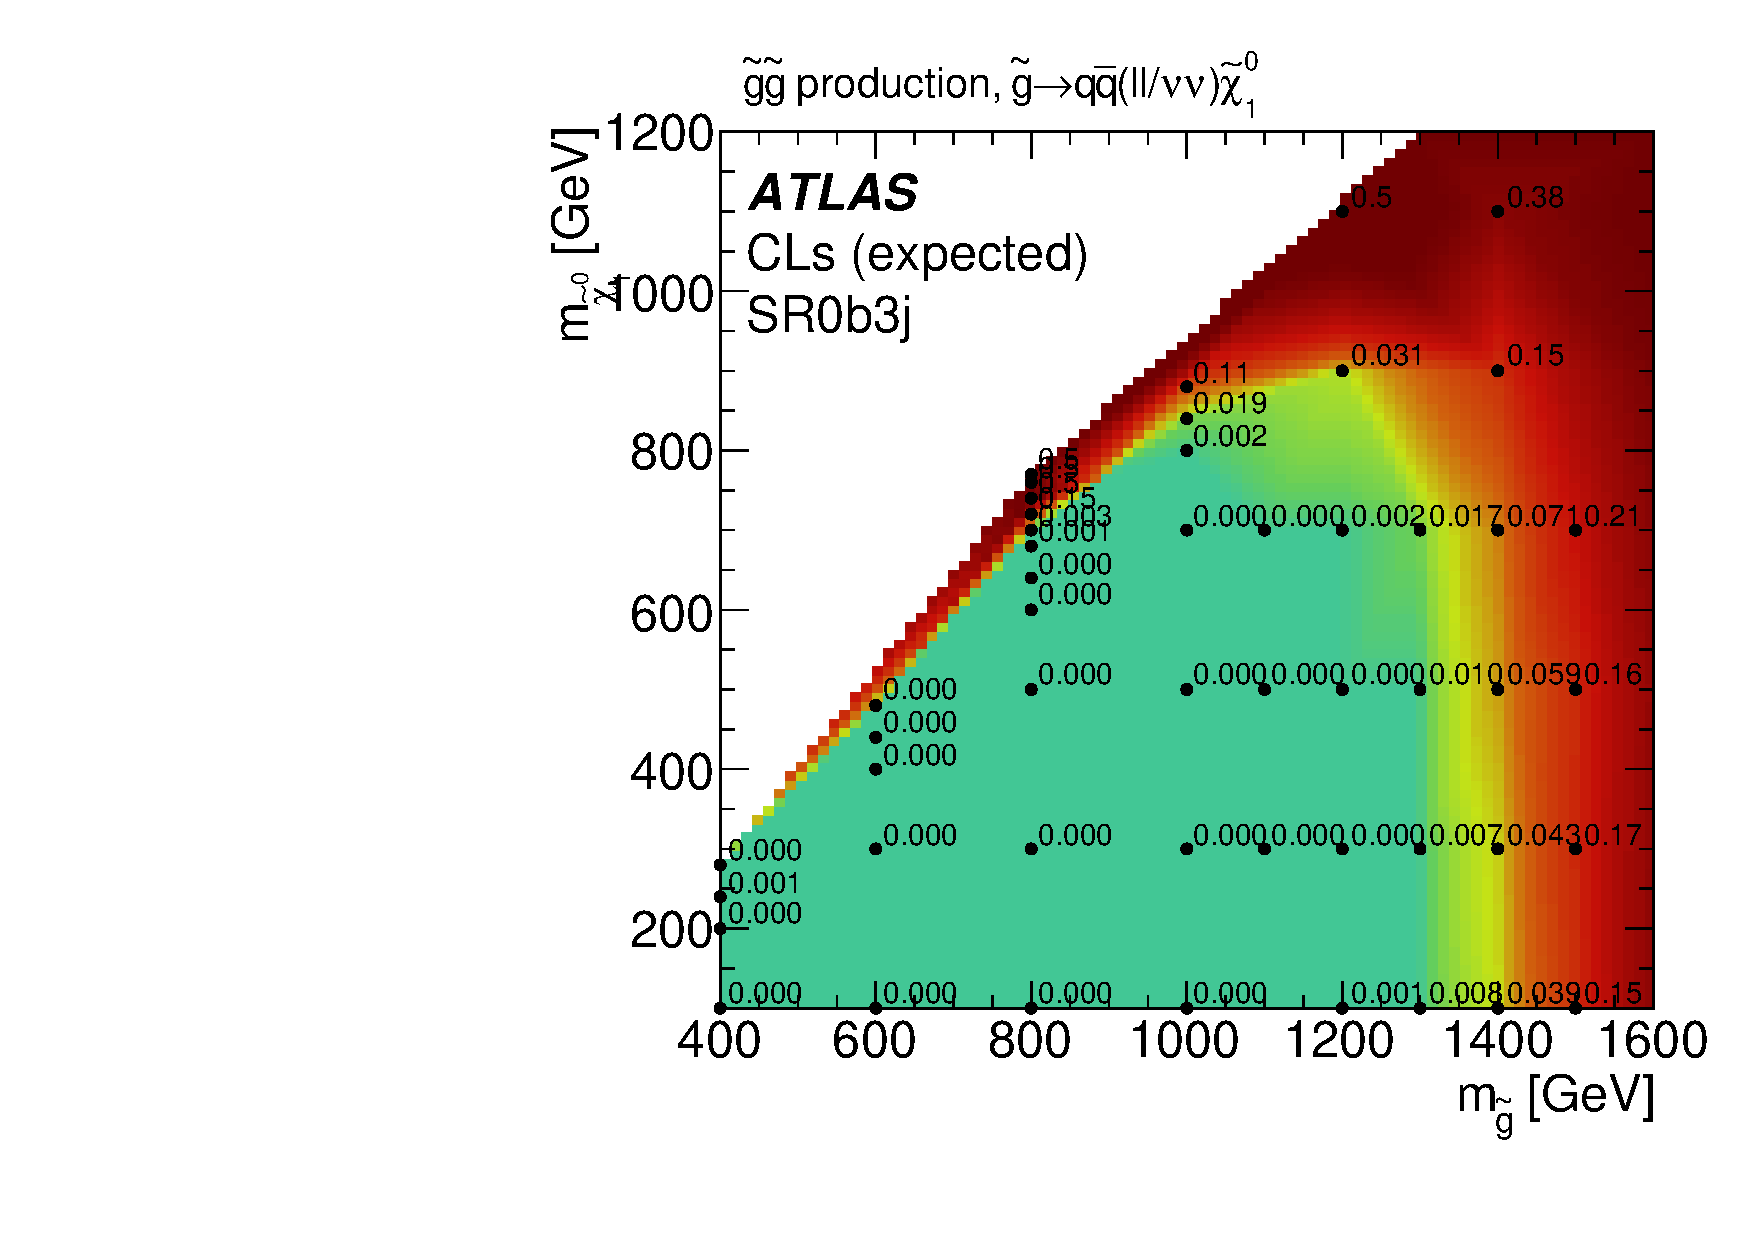
\includegraphics[width=\textwidth]{HEPDATA/clexp_SR0b3j.pdf}
\caption{$\gluino\to q\bar q \ell\ell\ninoone$ scenario, SR0b3j}\label{fig:hepdata_SR0b3j_CLexp}\end{subfigure}
\begin{subfigure}[t]{0.42\textwidth}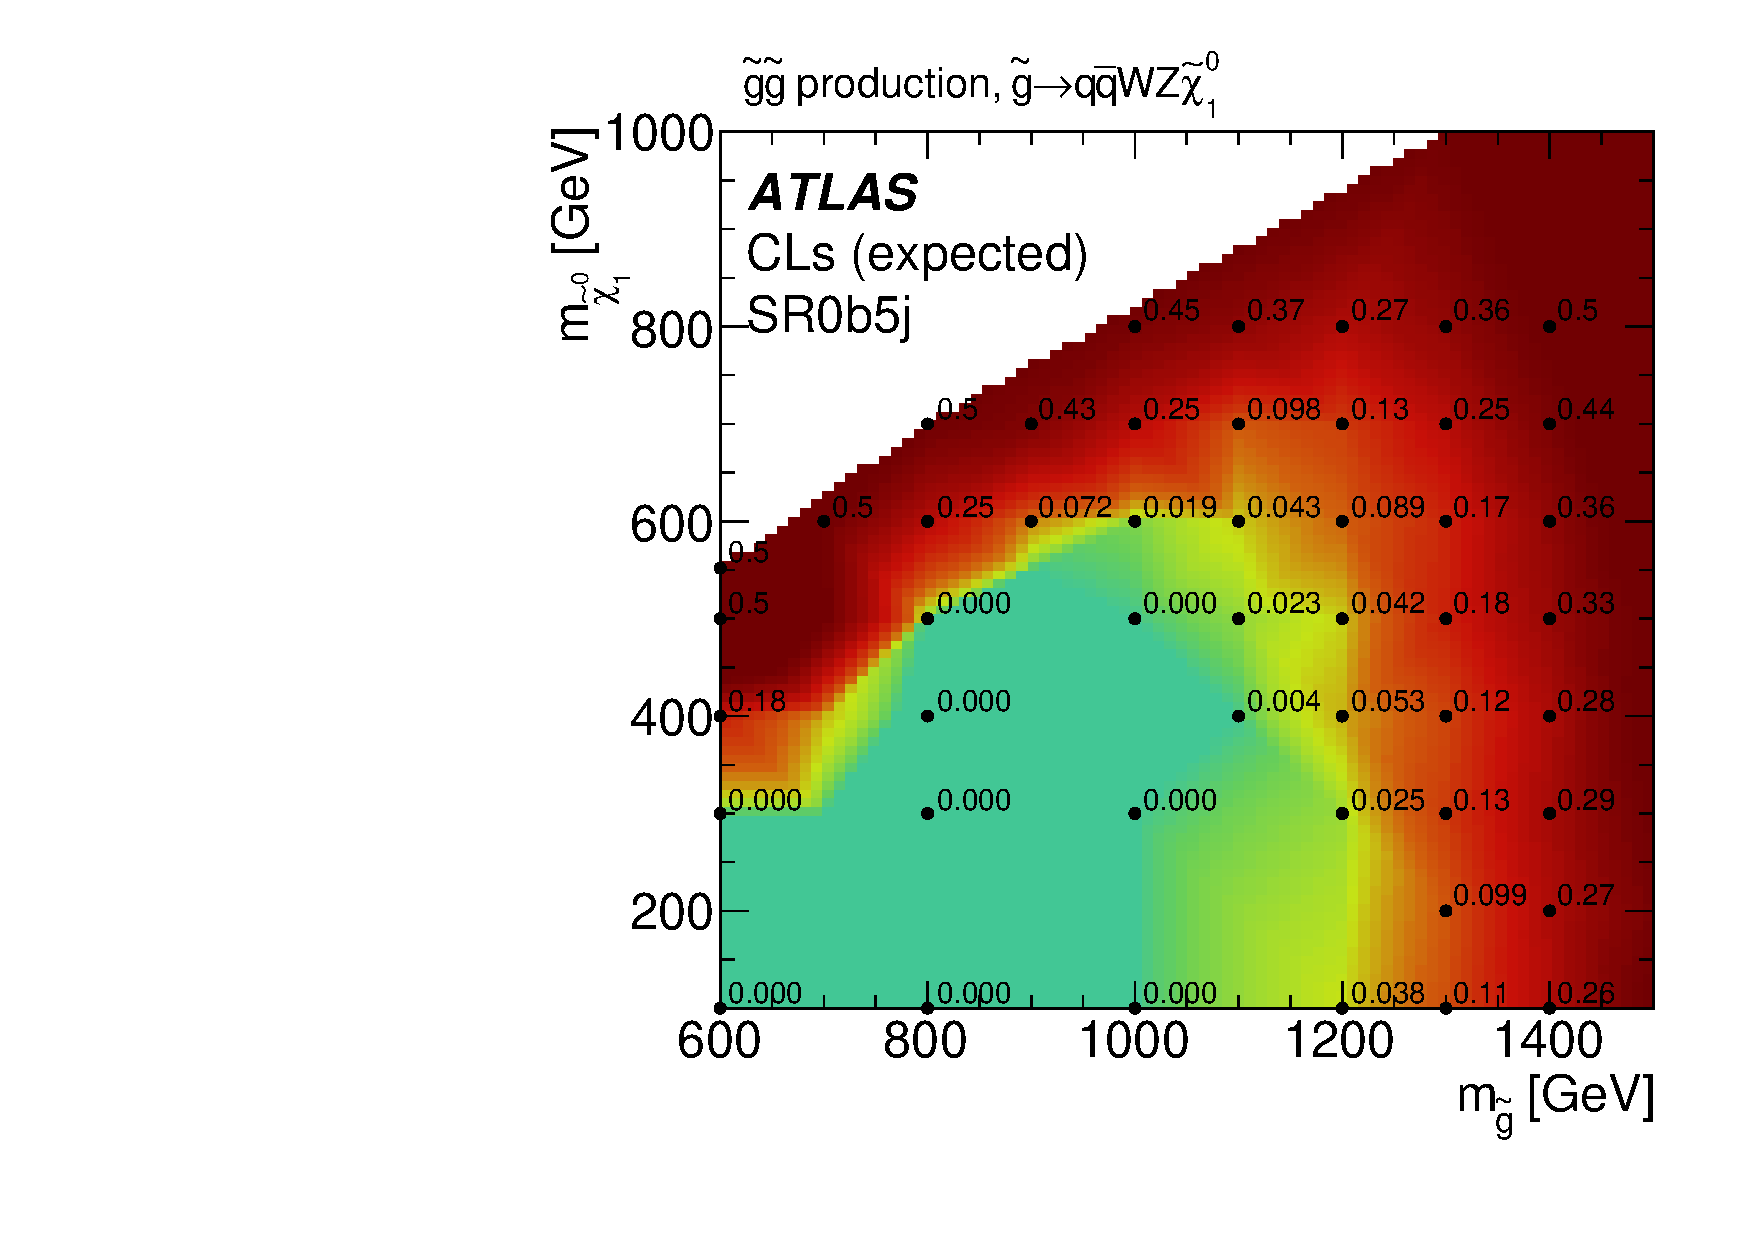
\includegraphics[width=\textwidth]{HEPDATA/clexp_SR0b5j.pdf}
\caption{$\gluino\to q\bar q' WZ\ninoone$ scenario, SR0b5j}\label{fig:hepdata_SR0b5j_CLexp}\end{subfigure}
\begin{subfigure}[t]{0.42\textwidth}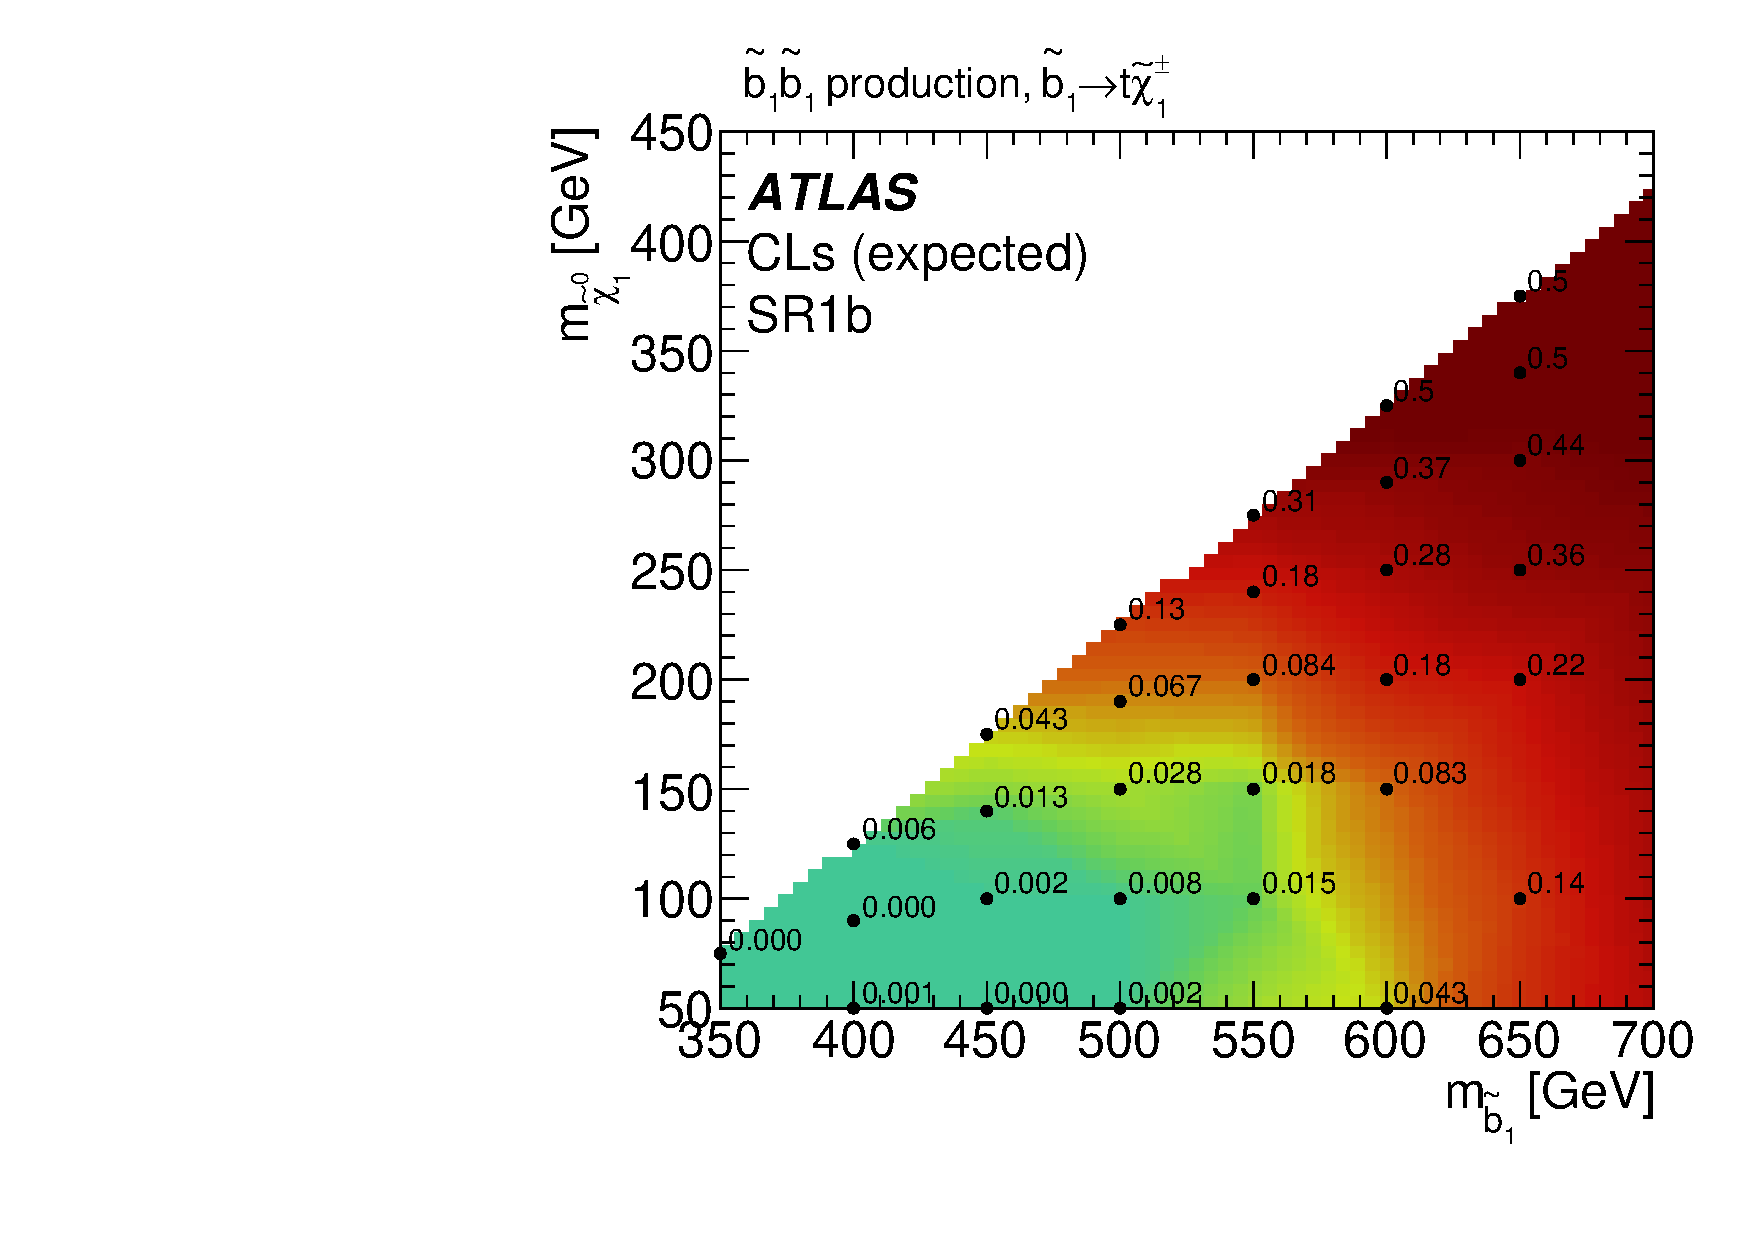
\includegraphics[width=\textwidth]{HEPDATA/clexp_SR1b.pdf}
\caption{$\sbottomone\to tW^-\ninoone$ scenario, SR1b}\label{fig:hepdata_SR1b_CLexp}\end{subfigure}
\begin{subfigure}[t]{0.42\textwidth}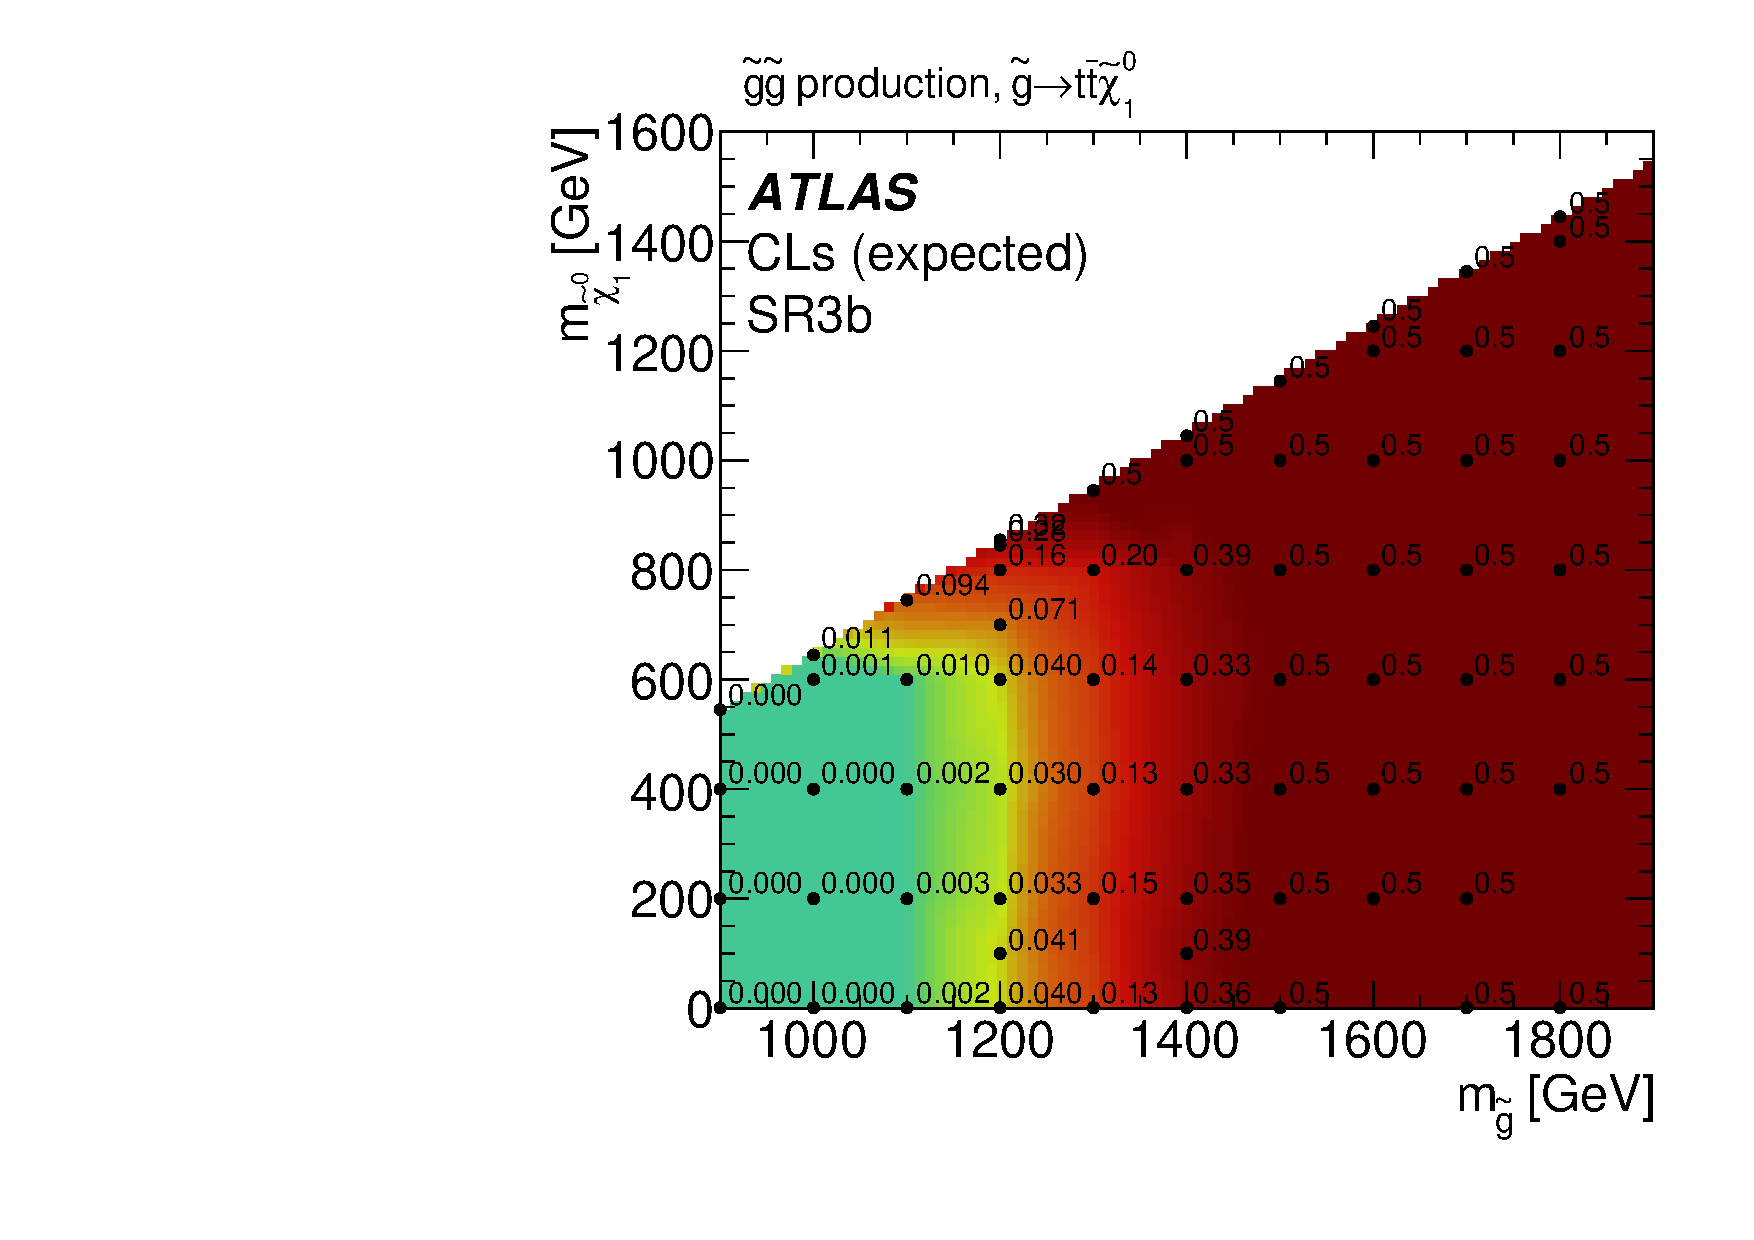
\includegraphics[width=\textwidth]{HEPDATA/clexp_SR3b.pdf}
\caption{$\gluino\to t\bar t\ninoone$ scenario, SR3b}\label{fig:hepdata_SR3b_CLexp}\end{subfigure}
\caption{Expected CL$_\mathrm{s}$ in the four signal regions. 
The benchmark scenarios used to set exclusion limits are materialized by black dot markers.}
\label{fig:HepData_CLexp} 
\end{figure} 

\begin{table}
\caption{Number of signal events selected at different stages of the signal regions definitions, 
for the four benchmark scenarios shown on Fig.~\ref{fig:Results_SR_metD}. 
Only the statistical uncertainties are displayed. }
\label{tab:signal_cutflow}
\centering
\begin{tabular}{|l|rc|}
\hline\hline
& Raw events & \begin{tabular}{@{}c@{}}Number of events expected\\ for $L=3.2$ fb$^{-1}$\end{tabular}\\
\hline\hline
\multicolumn{3}{|l|}{SR0b3j, $\gluino\to q\bar q(\ell\ell/\nu\nu)\ninoone$, $m_{\gluino}=\SI{1.3}{TeV}$, $m_{\ninoone}=\SI{500}{GeV}$} \\ \hline
produced									& 20051 	& 148 \\
$\ge 3$ leptons ($\pt>20,20,\SI{10}{GeV}$)	& 2026		& $14.4 \pm 0.4$\hspace*{1.95mm} \\
trigger										& 2024		& $14.3 \pm 0.4$\hspace*{1.95mm} \\
no $b$-jet ($\pt>\SI{20}{GeV}$)				& 1665		& $11.66 \pm 0.33$\hspace*{1.95mm} \\
$\ge 3$ jets ($\pt>\SI{50}{GeV}$)			& 1556		& $10.91 \pm 0.32$\hspace*{1.95mm} \\
$\met>\SI{200}{GeV}$						& 1079		& $7.52 \pm 0.27$ \\
$\meff>\SI{550}{GeV}$						& 1079		& $7.52 \pm 0.27$ \\
\hline\hline
\multicolumn{3}{|l|}{SR0b5j, $\gluino\to q\bar qWZ\ninoone$, $m_{\gluino}=\SI{1.1}{TeV}$, $m_{\ninoone}=\SI{400}{GeV}$} \\ \hline
produced									& 19000		& $524$ \\
$\ge 2$ SS leptons ($\pt>\SI{20}{GeV}$)		& 646		& $18.7 \pm 0.9$\hspace*{1.95mm} \\
trigger										& 631		& $17.8 \pm 0.9$\hspace*{1.95mm} \\
no $b$-jet ($\pt>\SI{20}{GeV}$)				& 419		& $11.4 \pm 0.7$\hspace*{1.95mm} \\
$\ge 5$ jets ($\pt>\SI{50}{GeV}$)			& 300		& $8.1 \pm 0.5$ \\
$\met>\SI{125}{GeV}$						& 252		& $6.7 \pm 0.5$ \\
$\meff>\SI{650}{GeV}$						& 252		& $6.7 \pm 0.5$ \\
\hline\hline
\multicolumn{3}{|l|}{SR1b, $\tilde{b}_1\to t\tilde{\chi}^{\pm}_{l}$, $m_{\tilde{b}_1}=\SI{600}{GeV}$, 
$m_{\tilde{\chi}^{\pm}_{l}}=\SI{150}{GeV}$, $m_{\ninoone}=\SI{50}{GeV}$} \\ \hline
produced									& 94706		& 560 \\
$\ge 2$ SS leptons ($\pt>\SI{20}{GeV}$)		& 4115		& $25.5 \pm 0.5$\hspace*{1.95mm} \\
trigger										& 3901		& $23.1 \pm 0.4$\hspace*{1.95mm} \\
$\ge 1$ $b$-jet ($\pt>\SI{20}{GeV}$)		& 3367		& $20.0 \pm 0.4$\hspace*{1.95mm} \\
$\ge 4$ jets ($\pt>\SI{50}{GeV}$)			& 1881		& $11.23 \pm 0.30$\hspace*{1.95mm} \\
$\met>\SI{150}{GeV}$						& 1148		& $7.08 \pm 0.24$ \\
$\meff>\SI{550}{GeV}$						& 1148		& $7.08 \pm 0.24$ \\
\hline\hline
\multicolumn{3}{|l|}{SR3b, $\gluino\to t\bar t\ninoone$, $m_{\gluino}=\SI{1.2}{TeV}$, $m_{\ninoone}=\SI{700}{GeV}$} \\ \hline
produced									& 100000	& 275 \\
$\ge 2$ SS leptons ($\pt>\SI{20}{GeV}$)		& 3535		& $9.28 \pm 0.18$ \\
trigger										& 3386		& $8.53 \pm 0.17$ \\
$\ge 3$ $b$-jets ($\pt>\SI{20}{GeV}$)		& 1704		& $4.26 \pm 0.12$ \\
$\met>\SI{125}{GeV}$						& 1320		& $3.31 \pm 0.11$ \\
$\meff>\SI{650}{GeV}$						& 1280		& $3.20 \pm 0.10$ \\
\hline\hline
\end{tabular}
\end{table}